\documentclass{book}
\usepackage[a4paper,top=2.5cm,bottom=2.5cm,left=2.5cm,right=2.5cm]{geometry}
\usepackage{makeidx}
\usepackage{natbib}
\usepackage{graphicx}
\usepackage{multicol}
\usepackage{float}
\usepackage{listings}
\usepackage{color}
\usepackage{ifthen}
\usepackage[table]{xcolor}
\usepackage{textcomp}
\usepackage{alltt}
\usepackage{ifpdf}
\ifpdf
\usepackage[pdftex,
            pagebackref=true,
            colorlinks=true,
            linkcolor=blue,
            unicode
           ]{hyperref}
\else
\usepackage[ps2pdf,
            pagebackref=true,
            colorlinks=true,
            linkcolor=blue,
            unicode
           ]{hyperref}
\usepackage{pspicture}
\fi
\usepackage[utf8]{inputenc}
\usepackage{mathptmx}
\usepackage[scaled=.90]{helvet}
\usepackage{courier}
\usepackage{sectsty}
\usepackage[titles]{tocloft}
\usepackage{doxygen}
\lstset{language=C++,inputencoding=utf8,basicstyle=\footnotesize,breaklines=true,breakatwhitespace=true,tabsize=4,numbers=left }
\makeindex
\setcounter{tocdepth}{3}
\renewcommand{\footrulewidth}{0.4pt}
\renewcommand{\familydefault}{\sfdefault}
\hfuzz=15pt
\setlength{\emergencystretch}{15pt}
\hbadness=750
\tolerance=750
\begin{document}
\hypersetup{pageanchor=false,citecolor=blue}
\begin{titlepage}
\vspace*{7cm}
\begin{center}
{\Large K\-Utils }\\
\vspace*{1cm}
{\large Generated by Doxygen 1.8.0}\\
\vspace*{0.5cm}
{\small Fri May 4 2012 17:51:37}\\
\end{center}
\end{titlepage}
\clearemptydoublepage
\pagenumbering{roman}
\tableofcontents
\clearemptydoublepage
\pagenumbering{arabic}
\hypersetup{pageanchor=true,citecolor=blue}
\chapter{Namespace Index}
\section{Namespace List}
Here is a list of all namespaces with brief descriptions\-:\begin{DoxyCompactList}
\item\contentsline{section}{\hyperlink{namespaceargparse}{argparse} \\*Command-\/line argument parser with a focus on brevity }{\pageref{namespaceargparse}}{}
\item\contentsline{section}{\hyperlink{namespaceautodiff}{autodiff} \\*Implements automatic differentiation }{\pageref{namespaceautodiff}}{}
\item\contentsline{section}{\hyperlink{namespacecvutils}{cvutils} \\*Open\-C\-V utilities }{\pageref{namespacecvutils}}{}
\item\contentsline{section}{\hyperlink{namespacecvutils_1_1geom}{cvutils\-::geom} \\*Operations on {\ttfamily cv\-::\-Point}s, {\ttfamily cv\-::\-Vec}s, and {\ttfamily cv\-::\-Rect}s }{\pageref{namespacecvutils_1_1geom}}{}
\item\contentsline{section}{\hyperlink{namespacecvutils_1_1transform}{cvutils\-::transform} \\*Functions related to affine transformations }{\pageref{namespacecvutils_1_1transform}}{}
\item\contentsline{section}{\hyperlink{namespacedict}{dict} \\*Utilities for working with {\ttfamily Dict}s ({\ttfamily unordered\-\_\-map}s) }{\pageref{namespacedict}}{}
\item\contentsline{section}{\hyperlink{namespacehumancv}{humancv} \\*Human-\/related computer vision utilities }{\pageref{namespacehumancv}}{}
\item\contentsline{section}{\hyperlink{namespacehumancv_1_1face}{humancv\-::face} \\*Basic face detection and modeling }{\pageref{namespacehumancv_1_1face}}{}
\item\contentsline{section}{\hyperlink{namespacehumancv_1_1skin}{humancv\-::skin} \\*Color-\/based skin segmentation }{\pageref{namespacehumancv_1_1skin}}{}
\item\contentsline{section}{\hyperlink{namespaceio}{io} \\*Convenience functions for printing values }{\pageref{namespaceio}}{}
\item\contentsline{section}{\hyperlink{namespacekmath}{kmath} \\*Miscellaneous mathematical functions }{\pageref{namespacekmath}}{}
\item\contentsline{section}{\hyperlink{namespacekrandom}{krandom} \\*Simple wrapper around {\ttfamily $<$random$>$} with a Python-\/like interface }{\pageref{namespacekrandom}}{}
\item\contentsline{section}{\hyperlink{namespacektime}{ktime} \\*Utilities for working with time }{\pageref{namespacektime}}{}
\item\contentsline{section}{\hyperlink{namespacemouse}{mouse} \\*Utilities for modeling the mouse state }{\pageref{namespacemouse}}{}
\item\contentsline{section}{\hyperlink{namespaceosx}{osx} \\*O\-S\-X-\/specific utilities }{\pageref{namespaceosx}}{}
\item\contentsline{section}{\hyperlink{namespaceosx_1_1disp}{osx\-::disp} \\*Functions for extracting the display image }{\pageref{namespaceosx_1_1disp}}{}
\item\contentsline{section}{\hyperlink{namespaceosx_1_1mouse}{osx\-::mouse} \\*Utilities for modeling the mouse state and controlling the mouse }{\pageref{namespaceosx_1_1mouse}}{}
\item\contentsline{section}{\hyperlink{namespaceosx__cv}{osx\-\_\-cv} \\*Functions for interoperability between Application\-Services and Open\-C\-V }{\pageref{namespaceosx__cv}}{}
\item\contentsline{section}{\hyperlink{namespaceseq}{seq} \\*Generic sequence operations and structures }{\pageref{namespaceseq}}{}
\item\contentsline{section}{\hyperlink{namespaceseq_1_1functional}{seq\-::functional} \\*Functions commonly used in functional programming }{\pageref{namespaceseq_1_1functional}}{}
\item\contentsline{section}{\hyperlink{namespaceseq_1_1math}{seq\-::math} \\*Mathematical operations on sequences, and sequence structures }{\pageref{namespaceseq_1_1math}}{}
\item\contentsline{section}{\hyperlink{namespacestr}{str} \\*String utilities }{\pageref{namespacestr}}{}
\item\contentsline{section}{\hyperlink{namespacethr}{thr} \\*Multi-\/threading utilities }{\pageref{namespacethr}}{}
\end{DoxyCompactList}

\chapter{Class Index}
\section{Class List}
Here are the classes, structs, unions and interfaces with brief descriptions\-:\begin{DoxyCompactList}
\item\contentsline{section}{\hyperlink{structcvutils_1_1___data_depth___fixed}{cvutils\-::\-\_\-\-Data\-Depth\-\_\-\-Fixed$<$ T $>$} \\*Get the number of bytes of a type at compile-\/time }{\pageref{structcvutils_1_1___data_depth___fixed}}{}
\item\contentsline{section}{\hyperlink{structcvutils_1_1___data_depth___fixed_3_01uchar_01_4}{cvutils\-::\-\_\-\-Data\-Depth\-\_\-\-Fixed$<$ uchar $>$} }{\pageref{structcvutils_1_1___data_depth___fixed_3_01uchar_01_4}}{}
\item\contentsline{section}{\hyperlink{structargparse_1_1_arg_holder}{argparse\-::\-Arg\-Holder} \\*Holds the result of parsing arguments }{\pageref{structargparse_1_1_arg_holder}}{}
\item\contentsline{section}{\hyperlink{classhumancv_1_1_cursor_finder}{humancv\-::\-Cursor\-Finder} \\*Framework for tracking hand gestures }{\pageref{classhumancv_1_1_cursor_finder}}{}
\item\contentsline{section}{\hyperlink{structautodiff_1_1_dual_num}{autodiff\-::\-Dual\-Num} \\*Represents the \char`\"{}real\char`\"{} part of a number in member {\ttfamily r} and the derivative in {\ttfamily d} }{\pageref{structautodiff_1_1_dual_num}}{}
\item\contentsline{section}{\hyperlink{structseq_1_1_elem_view}{seq\-::\-Elem\-View$<$ Seq\-T $>$} \\*Provides a reference and an index of an element in a sequence }{\pageref{structseq_1_1_elem_view}}{}
\item\contentsline{section}{\hyperlink{structhumancv_1_1_finger_data}{humancv\-::\-Finger\-Data} \\*Indices into a {\ttfamily Contour} denoting a finger }{\pageref{structhumancv_1_1_finger_data}}{}
\item\contentsline{section}{\hyperlink{structosx_1_1disp_1_1_image}{osx\-::disp\-::\-Image} }{\pageref{structosx_1_1disp_1_1_image}}{}
\item\contentsline{section}{\hyperlink{structkmath_1_1_interval}{kmath\-::\-Interval} \\*Represents an interval of real numbers }{\pageref{structkmath_1_1_interval}}{}
\item\contentsline{section}{\hyperlink{structosx_1_1mouse_1_1_mouse_state}{osx\-::mouse\-::\-Mouse\-State} \\*Simple data holder for a button flag and a position }{\pageref{structosx_1_1mouse_1_1_mouse_state}}{}
\item\contentsline{section}{\hyperlink{structkmath_1_1_point}{kmath\-::\-Point$<$ T $>$} \\*Generic point class }{\pageref{structkmath_1_1_point}}{}
\item\contentsline{section}{\hyperlink{structthr_1_1_queue}{thr\-::\-Queue$<$ T $>$} \\*Producer-\/consumer queue }{\pageref{structthr_1_1_queue}}{}
\item\contentsline{section}{\hyperlink{classktime_1_1_running_avg_timer}{ktime\-::\-Running\-Avg\-Timer} \\*Keep a running average of the time between calls to {\ttfamily \hyperlink{classktime_1_1_running_avg_timer_a1b28c95f0c44346321af8738e35f8025}{add\-Time()}} }{\pageref{classktime_1_1_running_avg_timer}}{}
\item\contentsline{section}{\hyperlink{structmouse_1_1_state}{mouse\-::\-State} \\*Simple data holder for a button flag and a position }{\pageref{structmouse_1_1_state}}{}
\item\contentsline{section}{\hyperlink{structcvutils_1_1_video_reader}{cvutils\-::\-Video\-Reader} \\*Represents a video input source (either a video file or camera) }{\pageref{structcvutils_1_1_video_reader}}{}
\item\contentsline{section}{\hyperlink{structseq_1_1_wrapped_seq}{seq\-::\-Wrapped\-Seq$<$ Seq\-T $>$} \\*Sequence wrapper that supports wrap-\/around indexing -\/ all accessors will accept negative and out-\/of-\/bound indices and wrap around }{\pageref{structseq_1_1_wrapped_seq}}{}
\item\contentsline{section}{\hyperlink{structseq_1_1math_1_1_x_range}{seq\-::math\-::\-X\-Range$<$ Num\-T $>$} \\*Represent a lazily-\/evaluated range of numbers }{\pageref{structseq_1_1math_1_1_x_range}}{}
\item\contentsline{section}{\hyperlink{classseq_1_1math_1_1_x_range_iterator}{seq\-::math\-::\-X\-Range\-Iterator$<$ Num\-T $>$} \\*Lazy iterator used for X\-Range(), usually not necessary to use directly }{\pageref{classseq_1_1math_1_1_x_range_iterator}}{}
\end{DoxyCompactList}

\chapter{File Index}
\section{File List}
Here is a list of all files with brief descriptions\-:\begin{DoxyCompactList}
\item\contentsline{section}{\hyperlink{argparse_8cpp}{argparse.\-cpp} }{\pageref{argparse_8cpp}}{}
\item\contentsline{section}{\hyperlink{argparse_8hpp}{argparse.\-hpp} }{\pageref{argparse_8hpp}}{}
\item\contentsline{section}{\hyperlink{autodiff_8cpp}{autodiff.\-cpp} }{\pageref{autodiff_8cpp}}{}
\item\contentsline{section}{\hyperlink{autodiff_8hpp}{autodiff.\-hpp} }{\pageref{autodiff_8hpp}}{}
\item\contentsline{section}{\hyperlink{cvutils_8cpp}{cvutils.\-cpp} }{\pageref{cvutils_8cpp}}{}
\item\contentsline{section}{\hyperlink{cvutils_8hpp}{cvutils.\-hpp} }{\pageref{cvutils_8hpp}}{}
\item\contentsline{section}{\hyperlink{dict_8hpp}{dict.\-hpp} }{\pageref{dict_8hpp}}{}
\item\contentsline{section}{\hyperlink{humancv_8cpp}{humancv.\-cpp} }{\pageref{humancv_8cpp}}{}
\item\contentsline{section}{\hyperlink{humancv_8hpp}{humancv.\-hpp} }{\pageref{humancv_8hpp}}{}
\item\contentsline{section}{\hyperlink{io_8hpp}{io.\-hpp} }{\pageref{io_8hpp}}{}
\item\contentsline{section}{\hyperlink{kmath_8cpp}{kmath.\-cpp} }{\pageref{kmath_8cpp}}{}
\item\contentsline{section}{\hyperlink{kmath_8hpp}{kmath.\-hpp} }{\pageref{kmath_8hpp}}{}
\item\contentsline{section}{\hyperlink{krandom_8cpp}{krandom.\-cpp} }{\pageref{krandom_8cpp}}{}
\item\contentsline{section}{\hyperlink{krandom_8hpp}{krandom.\-hpp} }{\pageref{krandom_8hpp}}{}
\item\contentsline{section}{\hyperlink{ktime_8cpp}{ktime.\-cpp} }{\pageref{ktime_8cpp}}{}
\item\contentsline{section}{\hyperlink{ktime_8hpp}{ktime.\-hpp} }{\pageref{ktime_8hpp}}{}
\item\contentsline{section}{\hyperlink{mouse_8cpp}{mouse.\-cpp} }{\pageref{mouse_8cpp}}{}
\item\contentsline{section}{\hyperlink{mouse_8hpp}{mouse.\-hpp} }{\pageref{mouse_8hpp}}{}
\item\contentsline{section}{\hyperlink{osx_8cpp}{osx.\-cpp} }{\pageref{osx_8cpp}}{}
\item\contentsline{section}{\hyperlink{osx_8hpp}{osx.\-hpp} }{\pageref{osx_8hpp}}{}
\item\contentsline{section}{\hyperlink{osx__cv_8cpp}{osx\-\_\-cv.\-cpp} }{\pageref{osx__cv_8cpp}}{}
\item\contentsline{section}{\hyperlink{osx__cv_8hpp}{osx\-\_\-cv.\-hpp} }{\pageref{osx__cv_8hpp}}{}
\item\contentsline{section}{\hyperlink{seq_8hpp}{seq.\-hpp} }{\pageref{seq_8hpp}}{}
\item\contentsline{section}{\hyperlink{str_8cpp}{str.\-cpp} }{\pageref{str_8cpp}}{}
\item\contentsline{section}{\hyperlink{str_8hpp}{str.\-hpp} }{\pageref{str_8hpp}}{}
\item\contentsline{section}{\hyperlink{thr_8hpp}{thr.\-hpp} }{\pageref{thr_8hpp}}{}
\end{DoxyCompactList}

\chapter{Namespace Documentation}
\hypertarget{namespaceargparse}{\section{argparse Namespace Reference}
\label{namespaceargparse}\index{argparse@{argparse}}
}


Command-\/line argument parser with a focus on brevity.  


\subsection*{Classes}
\begin{DoxyCompactItemize}
\item 
struct \hyperlink{structargparse_1_1_arg_holder}{Arg\-Holder}
\begin{DoxyCompactList}\small\item\em Holds the result of parsing arguments. \end{DoxyCompactList}\end{DoxyCompactItemize}
\subsection*{Functions}
\begin{DoxyCompactItemize}
\item 
string \hyperlink{namespaceargparse_a0ee3e8ca883816181b45c15a9ad0b6ed}{make\-Usage\-String} (const string \&prog\-Name, const string \&desc, const string \&pos\-Args=string(), const dict\-::\-Dict$<$ string, string $>$ \&opt\-To\-Help=dict\-::\-Dict$<$ string, string $>$(), unsigned cols=80, unsigned help\-Cols=60)
\begin{DoxyCompactList}\small\item\em Create a usage string. \end{DoxyCompactList}\item 
{\footnotesize template$<$class Func\-Type $>$ }\\\hyperlink{structargparse_1_1_arg_holder}{Arg\-Holder} \hyperlink{namespaceargparse_a4b1b6c03b45175acd13d1620f328e4aa}{parse} (int argc, const char $\ast$argv\mbox{[}$\,$\mbox{]}, const dict\-::\-Dict$<$ string, Func\-Type $>$ \&opt\-To\-Chker, char opt\-Char='-\/', bool gen\-Help\-Chker=true)
\begin{DoxyCompactList}\small\item\em Return an \hyperlink{structargparse_1_1_arg_holder}{Arg\-Holder} object holding the parsed arguments. \end{DoxyCompactList}\item 
\hyperlink{structargparse_1_1_arg_holder}{Arg\-Holder} \hyperlink{namespaceargparse_a6cfba06102a610840779069dfda1b98d}{parse} (int argc, const char $\ast$argv\mbox{[}$\,$\mbox{]}, const char opt\-Char='-\/', bool gen\-Help\-Chker=true)
\begin{DoxyCompactList}\small\item\em For programs that take no options. \end{DoxyCompactList}\end{DoxyCompactItemize}


\subsection{Detailed Description}
Command-\/line argument parser with a focus on brevity. 

\subsection{Function Documentation}
\hypertarget{namespaceargparse_a0ee3e8ca883816181b45c15a9ad0b6ed}{\index{argparse@{argparse}!make\-Usage\-String@{make\-Usage\-String}}
\index{make\-Usage\-String@{make\-Usage\-String}!argparse@{argparse}}
\subsubsection[{make\-Usage\-String}]{\setlength{\rightskip}{0pt plus 5cm}string {\bf argparse\-::make\-Usage\-String} (
\begin{DoxyParamCaption}
\item[{const string \&}]{prog\-Name, }
\item[{const string \&}]{desc, }
\item[{const string \&}]{pos\-Args = {\ttfamily string()}, }
\item[{const dict\-::\-Dict$<$ string, string $>$ \&}]{opt\-To\-Help = {\ttfamily dict\-:\-:Dict$<$string,~string$>$()}, }
\item[{unsigned}]{cols = {\ttfamily 80}, }
\item[{unsigned}]{help\-Cols = {\ttfamily 60}}
\end{DoxyParamCaption}
)}}\label{namespaceargparse_a0ee3e8ca883816181b45c15a9ad0b6ed}


Create a usage string. 


\begin{DoxyParams}{Parameters}
{\em prog\-Name} & Name of the program as run on the command line. Typically {\ttfamily argv\mbox{[}0\mbox{]}} is passed. \\
\hline
{\em desc} & Description of the program. \\
\hline
{\em pos\-Args} & String representing the positional arguments. \\
\hline
{\em opt\-To\-Help} & Mapping from option to help dialog. \\
\hline
{\em cols} & Maximum number of columns -\/ strings longer than this will be wrapped. \\
\hline
{\em help\-Cols} & Number of columns that the option help should take up.\\
\hline
\end{DoxyParams}
Example\-: \begin{DoxyVerb} makeUsageString(
         "testprog",
         "This is a description of the program.",
         "arg1 arg2 arg3",
         makeDict(
             string("-h"), string("print a help message"),
             string("-a"), string("add some numbers")
             )
         )\end{DoxyVerb}
 generates this help string\-: \begin{DoxyVerb} Usage: testprog [options] arg1 arg2 arg3

 This is a description of the program.

 Options:
 -a                  add some numbers
 -h                  print a help message\end{DoxyVerb}
 \hypertarget{namespaceargparse_a4b1b6c03b45175acd13d1620f328e4aa}{\index{argparse@{argparse}!parse@{parse}}
\index{parse@{parse}!argparse@{argparse}}
\subsubsection[{parse}]{\setlength{\rightskip}{0pt plus 5cm}template$<$class Func\-Type $>$ {\bf Arg\-Holder} {\bf argparse\-::parse} (
\begin{DoxyParamCaption}
\item[{int}]{argc, }
\item[{const char $\ast$}]{argv\mbox{[}$\,$\mbox{]}, }
\item[{const dict\-::\-Dict$<$ string, Func\-Type $>$ \&}]{opt\-To\-Chker, }
\item[{char}]{opt\-Char = {\ttfamily '-\/'}, }
\item[{bool}]{gen\-Help\-Chker = {\ttfamily true}}
\end{DoxyParamCaption}
)}}\label{namespaceargparse_a4b1b6c03b45175acd13d1620f328e4aa}


Return an \hyperlink{structargparse_1_1_arg_holder}{Arg\-Holder} object holding the parsed arguments. 


\begin{DoxyParams}{Parameters}
{\em argc,argv} & The arguments to main(). \\
\hline
{\em opt\-To\-Chker} & Should map an option string (anything beginning with {\ttfamily opt\-Char}) to a checker function that takes a vector of argument strings and returns the number of arguments read. The function should also throw an {\ttfamily invalid\-\_\-argument} exception if any arguments are invalid. For example, a simple help option checker\-: \begin{DoxyVerb}makeDict(string("-h"), [](vector<string> args) { return 0; })
\end{DoxyVerb}
 \\
\hline
{\em opt\-Char} & Signifies the start of an option. \\
\hline
{\em gen\-Help\-Chker} & If {\ttfamily true}, checks \char`\"{}-\/h\char`\"{} and \char`\"{}-\/-\/help\char`\"{} options automatically.\\
\hline
\end{DoxyParams}

\begin{DoxyExceptions}{Exceptions}
{\em invalid\-\_\-argument} & Thrown if unknown option is encountered, as well as if a checker throws an {\ttfamily invalid\-\_\-argument} exception. \\
\hline
\end{DoxyExceptions}
\hypertarget{namespaceargparse_a6cfba06102a610840779069dfda1b98d}{\index{argparse@{argparse}!parse@{parse}}
\index{parse@{parse}!argparse@{argparse}}
\subsubsection[{parse}]{\setlength{\rightskip}{0pt plus 5cm}{\bf Arg\-Holder} {\bf argparse\-::parse} (
\begin{DoxyParamCaption}
\item[{int}]{argc, }
\item[{const char $\ast$}]{argv\mbox{[}$\,$\mbox{]}, }
\item[{const char}]{opt\-Char = {\ttfamily '-\/'}, }
\item[{bool}]{gen\-Help\-Chker = {\ttfamily true}}
\end{DoxyParamCaption}
)}}\label{namespaceargparse_a6cfba06102a610840779069dfda1b98d}


For programs that take no options. 

See \hyperlink{namespaceargparse_a4b1b6c03b45175acd13d1620f328e4aa}{parse()} above. 
\hypertarget{namespaceautodiff}{\section{autodiff Namespace Reference}
\label{namespaceautodiff}\index{autodiff@{autodiff}}
}


Implements automatic differentiation.  


\subsection*{Classes}
\begin{DoxyCompactItemize}
\item 
struct \hyperlink{structautodiff_1_1_dual_num}{Dual\-Num}
\begin{DoxyCompactList}\small\item\em Represents the \char`\"{}real\char`\"{} part of a number in member {\ttfamily r} and the derivative in {\ttfamily d}. \end{DoxyCompactList}\end{DoxyCompactItemize}
\subsection*{Functions}
\begin{DoxyCompactItemize}
\item 
\hyperlink{structautodiff_1_1_dual_num}{Dual\-Num} \hyperlink{namespaceautodiff_a19b889e35f523cc6ca0f377dc8bed262}{d\-Pow} (const \hyperlink{structautodiff_1_1_dual_num}{Dual\-Num} \&a, const \hyperlink{structautodiff_1_1_dual_num}{Dual\-Num} \&b)
\item 
\hyperlink{structautodiff_1_1_dual_num}{Dual\-Num} \hyperlink{namespaceautodiff_a0f6df25515f7f05f838a9fd96f53fd37}{d\-Sin} (const \hyperlink{structautodiff_1_1_dual_num}{Dual\-Num} \&a)
\item 
\hyperlink{structautodiff_1_1_dual_num}{Dual\-Num} \hyperlink{namespaceautodiff_a49d66a6f54fffb4250795cc589158a14}{d\-Cos} (const \hyperlink{structautodiff_1_1_dual_num}{Dual\-Num} \&a)
\item 
\hyperlink{structautodiff_1_1_dual_num}{Dual\-Num} \hyperlink{namespaceautodiff_a4bdb0754d9ad8a5c4aba2d7ea9f040db}{d\-Tan} (const \hyperlink{structautodiff_1_1_dual_num}{Dual\-Num} \&a)
\item 
\hyperlink{structautodiff_1_1_dual_num}{Dual\-Num} \hyperlink{namespaceautodiff_af2706967e031d3472b823760b0c67dcb}{d\-Exp} (const \hyperlink{structautodiff_1_1_dual_num}{Dual\-Num} \&a)
\item 
\hyperlink{structautodiff_1_1_dual_num}{Dual\-Num} \hyperlink{namespaceautodiff_a003e7455b4727bad71fdb9b6bc676e86}{d\-Log} (const \hyperlink{structautodiff_1_1_dual_num}{Dual\-Num} \&a)
\item 
\hyperlink{structautodiff_1_1_dual_num}{Dual\-Num} \hyperlink{namespaceautodiff_a656dafc1fc9422d40ade97d24905f875}{d\-Log10} (const \hyperlink{structautodiff_1_1_dual_num}{Dual\-Num} \&a)
\end{DoxyCompactItemize}
\subsection*{Variables}
\begin{DoxyCompactItemize}
\item 
const double \hyperlink{namespaceautodiff_ac438d71cd4847e9f19efe6a4f1cfd5d7}{I\-N\-V\-\_\-\-L\-O\-G\-\_\-10} = 1 / log(10)
\end{DoxyCompactItemize}


\subsection{Detailed Description}
Implements automatic differentiation. See\-: \href{http://www.pvv.ntnu.no/~berland/resources/autodiff-triallecture.pdf}{\tt http\-://www.\-pvv.\-ntnu.\-no/$\sim$berland/resources/autodiff-\/triallecture.\-pdf}

Many but not all of the functions in the {\ttfamily cmath} library are implemented with a {\ttfamily d$\ast$} prefix, eg. {\ttfamily d\-Sin}. 

\subsection{Function Documentation}
\hypertarget{namespaceautodiff_a19b889e35f523cc6ca0f377dc8bed262}{\index{autodiff@{autodiff}!d\-Pow@{d\-Pow}}
\index{d\-Pow@{d\-Pow}!autodiff@{autodiff}}
\subsubsection[{d\-Pow}]{\setlength{\rightskip}{0pt plus 5cm}{\bf Dual\-Num} {\bf autodiff\-::d\-Pow} (
\begin{DoxyParamCaption}
\item[{const {\bf Dual\-Num} \&}]{a, }
\item[{const {\bf Dual\-Num} \&}]{b}
\end{DoxyParamCaption}
)}}\label{namespaceautodiff_a19b889e35f523cc6ca0f377dc8bed262}
\hypertarget{namespaceautodiff_a0f6df25515f7f05f838a9fd96f53fd37}{\index{autodiff@{autodiff}!d\-Sin@{d\-Sin}}
\index{d\-Sin@{d\-Sin}!autodiff@{autodiff}}
\subsubsection[{d\-Sin}]{\setlength{\rightskip}{0pt plus 5cm}{\bf Dual\-Num} {\bf autodiff\-::d\-Sin} (
\begin{DoxyParamCaption}
\item[{const {\bf Dual\-Num} \&}]{a}
\end{DoxyParamCaption}
)}}\label{namespaceautodiff_a0f6df25515f7f05f838a9fd96f53fd37}
\hypertarget{namespaceautodiff_a49d66a6f54fffb4250795cc589158a14}{\index{autodiff@{autodiff}!d\-Cos@{d\-Cos}}
\index{d\-Cos@{d\-Cos}!autodiff@{autodiff}}
\subsubsection[{d\-Cos}]{\setlength{\rightskip}{0pt plus 5cm}{\bf Dual\-Num} {\bf autodiff\-::d\-Cos} (
\begin{DoxyParamCaption}
\item[{const {\bf Dual\-Num} \&}]{a}
\end{DoxyParamCaption}
)}}\label{namespaceautodiff_a49d66a6f54fffb4250795cc589158a14}
\hypertarget{namespaceautodiff_a4bdb0754d9ad8a5c4aba2d7ea9f040db}{\index{autodiff@{autodiff}!d\-Tan@{d\-Tan}}
\index{d\-Tan@{d\-Tan}!autodiff@{autodiff}}
\subsubsection[{d\-Tan}]{\setlength{\rightskip}{0pt plus 5cm}{\bf Dual\-Num} {\bf autodiff\-::d\-Tan} (
\begin{DoxyParamCaption}
\item[{const {\bf Dual\-Num} \&}]{a}
\end{DoxyParamCaption}
)}}\label{namespaceautodiff_a4bdb0754d9ad8a5c4aba2d7ea9f040db}
\hypertarget{namespaceautodiff_af2706967e031d3472b823760b0c67dcb}{\index{autodiff@{autodiff}!d\-Exp@{d\-Exp}}
\index{d\-Exp@{d\-Exp}!autodiff@{autodiff}}
\subsubsection[{d\-Exp}]{\setlength{\rightskip}{0pt plus 5cm}{\bf Dual\-Num} {\bf autodiff\-::d\-Exp} (
\begin{DoxyParamCaption}
\item[{const {\bf Dual\-Num} \&}]{a}
\end{DoxyParamCaption}
)}}\label{namespaceautodiff_af2706967e031d3472b823760b0c67dcb}
\hypertarget{namespaceautodiff_a003e7455b4727bad71fdb9b6bc676e86}{\index{autodiff@{autodiff}!d\-Log@{d\-Log}}
\index{d\-Log@{d\-Log}!autodiff@{autodiff}}
\subsubsection[{d\-Log}]{\setlength{\rightskip}{0pt plus 5cm}{\bf Dual\-Num} {\bf autodiff\-::d\-Log} (
\begin{DoxyParamCaption}
\item[{const {\bf Dual\-Num} \&}]{a}
\end{DoxyParamCaption}
)}}\label{namespaceautodiff_a003e7455b4727bad71fdb9b6bc676e86}
\hypertarget{namespaceautodiff_a656dafc1fc9422d40ade97d24905f875}{\index{autodiff@{autodiff}!d\-Log10@{d\-Log10}}
\index{d\-Log10@{d\-Log10}!autodiff@{autodiff}}
\subsubsection[{d\-Log10}]{\setlength{\rightskip}{0pt plus 5cm}{\bf Dual\-Num} {\bf autodiff\-::d\-Log10} (
\begin{DoxyParamCaption}
\item[{const {\bf Dual\-Num} \&}]{a}
\end{DoxyParamCaption}
)}}\label{namespaceautodiff_a656dafc1fc9422d40ade97d24905f875}


\subsection{Variable Documentation}
\hypertarget{namespaceautodiff_ac438d71cd4847e9f19efe6a4f1cfd5d7}{\index{autodiff@{autodiff}!I\-N\-V\-\_\-\-L\-O\-G\-\_\-10@{I\-N\-V\-\_\-\-L\-O\-G\-\_\-10}}
\index{I\-N\-V\-\_\-\-L\-O\-G\-\_\-10@{I\-N\-V\-\_\-\-L\-O\-G\-\_\-10}!autodiff@{autodiff}}
\subsubsection[{I\-N\-V\-\_\-\-L\-O\-G\-\_\-10}]{\setlength{\rightskip}{0pt plus 5cm}const double {\bf autodiff\-::\-I\-N\-V\-\_\-\-L\-O\-G\-\_\-10} = 1 / log(10)}}\label{namespaceautodiff_ac438d71cd4847e9f19efe6a4f1cfd5d7}

\hypertarget{namespacecvutils}{\section{cvutils Namespace Reference}
\label{namespacecvutils}\index{cvutils@{cvutils}}
}


Open\-C\-V utilities.  


\subsection*{Namespaces}
\begin{DoxyCompactItemize}
\item 
namespace \hyperlink{namespacecvutils_1_1geom}{geom}
\begin{DoxyCompactList}\small\item\em Operations on {\ttfamily cv\-::\-Point}s, {\ttfamily cv\-::\-Vec}s, and {\ttfamily cv\-::\-Rect}s. \end{DoxyCompactList}\item 
namespace \hyperlink{namespacecvutils_1_1transform}{transform}
\begin{DoxyCompactList}\small\item\em Functions related to affine transformations. \end{DoxyCompactList}\end{DoxyCompactItemize}
\subsection*{Classes}
\begin{DoxyCompactItemize}
\item 
struct \hyperlink{structcvutils_1_1___data_depth___fixed}{\-\_\-\-Data\-Depth\-\_\-\-Fixed}
\begin{DoxyCompactList}\small\item\em Get the number of bytes of a type at compile-\/time. \end{DoxyCompactList}\item 
struct \hyperlink{structcvutils_1_1___data_depth___fixed_3_01uchar_01_4}{\-\_\-\-Data\-Depth\-\_\-\-Fixed$<$ uchar $>$}
\item 
struct \hyperlink{structcvutils_1_1_video_reader}{Video\-Reader}
\begin{DoxyCompactList}\small\item\em Represents a video input source (either a video file or camera). \end{DoxyCompactList}\end{DoxyCompactItemize}
\subsection*{Enumerations}
\begin{DoxyCompactItemize}
\item 
enum \hyperlink{namespacecvutils_a955c1d8733f727414da8a357b938ced7}{X\-Loc} \{ \hyperlink{namespacecvutils_a955c1d8733f727414da8a357b938ced7a6a9a0a917be940c0641d145580dcf0f7}{F\-I\-X\-\_\-\-C\-E\-N\-T\-E\-R\-\_\-\-X}, 
\hyperlink{namespacecvutils_a955c1d8733f727414da8a357b938ced7a2557bbfc7f88e4a68d6ed50b1f59df49}{F\-I\-X\-\_\-\-L\-E\-F\-T}, 
\hyperlink{namespacecvutils_a955c1d8733f727414da8a357b938ced7afb4808b8ea22de530ed6c9bc7198161a}{F\-I\-X\-\_\-\-R\-I\-G\-H\-T}
 \}
\begin{DoxyCompactList}\small\item\em Specifies positions for affixing {\ttfamily cv\-::\-Rect}s or {\ttfamily cv\-::\-Size}s. \end{DoxyCompactList}\item 
enum \hyperlink{namespacecvutils_a0a32f5be1c20397001a2cdc59bacec81}{Y\-Loc} \{ \hyperlink{namespacecvutils_a0a32f5be1c20397001a2cdc59bacec81ad6382055c3ad3cb882f8f123e3b64f38}{F\-I\-X\-\_\-\-C\-E\-N\-T\-E\-R\-\_\-\-Y}, 
\hyperlink{namespacecvutils_a0a32f5be1c20397001a2cdc59bacec81a1ef7dcf2027f67cb73fe3c2b8283e680}{F\-I\-X\-\_\-\-T\-O\-P}, 
\hyperlink{namespacecvutils_a0a32f5be1c20397001a2cdc59bacec81a3f77fa48f399deb5768cbcf63d1f9eae}{F\-I\-X\-\_\-\-B\-O\-T\-T\-O\-M}
 \}
\end{DoxyCompactItemize}
\subsection*{Functions}
\begin{DoxyCompactItemize}
\item 
void \hyperlink{namespacecvutils_aa292da4b50c7692374fdde56afdd6baf}{wait\-For\-Keypress} ()
\begin{DoxyCompactList}\small\item\em Block until a key is pressed. \end{DoxyCompactList}\item 
{\footnotesize template$<$typename T $>$ }\\cv\-::\-Point \hyperlink{namespacecvutils_a828567eec14cbe1369c315d025f108ba}{to\-C\-V\-Pt} (\hyperlink{structkmath_1_1_point}{kmath\-::\-Point}$<$ T $>$ pt)
\begin{DoxyCompactList}\small\item\em Convert a {\ttfamily \hyperlink{structkmath_1_1_point}{kmath\-::\-Point}$<$T$>$} to a {\ttfamily cv\-::\-Point}. \end{DoxyCompactList}\item 
{\footnotesize template$<$typename T $>$ }\\\hyperlink{structkmath_1_1_point}{kmath\-::\-Point}$<$ T $>$ \hyperlink{namespacecvutils_ab27154874f930e865580b2b3c6afead5}{to\-C\-G\-Pt} (cv\-::\-Point pt)
\begin{DoxyCompactList}\small\item\em Convert a {\ttfamily cv\-::\-Point} to a {\ttfamily \hyperlink{structkmath_1_1_point}{kmath\-::\-Point}$<$T$>$}. \end{DoxyCompactList}\item 
{\footnotesize template$<$typename T1 , typename T2 , typename \-\_\-\-Func\-T $>$ }\\void \hyperlink{namespacecvutils_a9a51cd204369adbf1321482a67c101dc}{apply\-Binary\-Op} (const \-\_\-\-Func\-T \&func, cv\-::\-Mat\-\_\-$<$ T1 $>$ \&m1, cv\-::\-Mat\-\_\-$<$ T2 $>$ \&m2)
\begin{DoxyCompactList}\small\item\em For each pixel in {\ttfamily m1} and {\ttfamily m2}, call\-: \end{DoxyCompactList}\item 
{\footnotesize template$<$typename T1 , typename T2 , typename \-\_\-\-Func\-T $>$ }\\void \hyperlink{namespacecvutils_a624390fc5d29f7ca9f2342f6ae7849be}{apply\-Binary\-Op} (const \-\_\-\-Func\-T \&func, const cv\-::\-Mat\-\_\-$<$ T1 $>$ \&m1, cv\-::\-Mat\-\_\-$<$ T2 $>$ \&m2)
\begin{DoxyCompactList}\small\item\em Partly const version of \hyperlink{namespacecvutils_a9a51cd204369adbf1321482a67c101dc}{apply\-Binary\-Op()}. \end{DoxyCompactList}\item 
{\footnotesize template$<$typename T1 , typename T2 , typename \-\_\-\-Func\-T $>$ }\\void \hyperlink{namespacecvutils_a18bf9198d170d4f95ebeda01c4c66b48}{apply\-Binary\-Op} (const \-\_\-\-Func\-T \&func, cv\-::\-Mat\-\_\-$<$ T1 $>$ \&m1, const cv\-::\-Mat\-\_\-$<$ T2 $>$ \&m2)
\begin{DoxyCompactList}\small\item\em Partly const version of \hyperlink{namespacecvutils_a9a51cd204369adbf1321482a67c101dc}{apply\-Binary\-Op()}. \end{DoxyCompactList}\item 
{\footnotesize template$<$typename T1 , typename T2 , typename \-\_\-\-Func\-T $>$ }\\void \hyperlink{namespacecvutils_a7de5d736aac8827c278399e59cdb62ce}{apply\-Binary\-Op} (const \-\_\-\-Func\-T \&func, const cv\-::\-Mat\-\_\-$<$ T1 $>$ \&m1, const cv\-::\-Mat\-\_\-$<$ T2 $>$ \&m2)
\begin{DoxyCompactList}\small\item\em Const version of \hyperlink{namespacecvutils_a9a51cd204369adbf1321482a67c101dc}{apply\-Binary\-Op()}. \end{DoxyCompactList}\item 
cv\-::\-Scalar \hyperlink{namespacecvutils_abcad4782a40d57854115ea2dcdab401b}{rand\-Color} ()
\begin{DoxyCompactList}\small\item\em Return a random R\-G\-B color as a cv\-::\-Scalar. \end{DoxyCompactList}\item 
void \hyperlink{namespacecvutils_a683e21d8e2c62e903c76ae0279e4a94d}{draw\-Polygon} (cv\-::\-Mat \&im, const vector$<$ cv\-::\-Point $>$ \&pts, const cv\-::\-Scalar \&color=cv\-::\-Scalar(255, 255, 255), int thickness=1, int line\-Type=8, bool convex=true)
\begin{DoxyCompactList}\small\item\em Draw the outline of a closed polygon specified by {\ttfamily pts} on {\ttfamily im}. \end{DoxyCompactList}\item 
void \hyperlink{namespacecvutils_ada4f02293fd7783beff2240b94d625a7}{expand\-Mat} (const cv\-::\-Mat \&src, cv\-::\-Mat \&dest, cv\-::\-Size new\-Size, cv\-::\-Point offset, cv\-::\-Scalar fill\-Val=cv\-::\-Scalar())
\begin{DoxyCompactList}\small\item\em Pad {\ttfamily src} to a larger size and store in {\ttfamily dest}, filling extra space with {\ttfamily fill\-Val}. \end{DoxyCompactList}\item 
void \hyperlink{namespacecvutils_a128502dc926237b41ee2598574a4b409}{expand\-Mat} (const cv\-::\-Mat \&src, cv\-::\-Mat \&dest, cv\-::\-Size new\-Size, cv\-::\-Scalar fill\-Val=cv\-::\-Scalar(), \hyperlink{namespacecvutils_a955c1d8733f727414da8a357b938ced7}{X\-Loc} x\-Flag=\hyperlink{namespacecvutils_a955c1d8733f727414da8a357b938ced7a6a9a0a917be940c0641d145580dcf0f7}{F\-I\-X\-\_\-\-C\-E\-N\-T\-E\-R\-\_\-\-X}, \hyperlink{namespacecvutils_a0a32f5be1c20397001a2cdc59bacec81}{Y\-Loc} y\-Flag=\hyperlink{namespacecvutils_a0a32f5be1c20397001a2cdc59bacec81ad6382055c3ad3cb882f8f123e3b64f38}{F\-I\-X\-\_\-\-C\-E\-N\-T\-E\-R\-\_\-\-Y})
\item 
void \hyperlink{namespacecvutils_afce5aa1e29332624c3f7cbabcbe19f69}{cvt\-B\-G\-R2\-R\-G} (const cv\-::\-Mat \&src, cv\-::\-Mat \&dest)
\begin{DoxyCompactList}\small\item\em Convert a matrix from B\-G\-R color space to rg chromaticity space, with the 3rd channel unused. \end{DoxyCompactList}\item 
void \hyperlink{namespacecvutils_aa787df79b1daecd591a52fd071ac5618}{face\-Detect\-Scaled} (const cv\-::\-Mat \&src, float scale, vector$<$ cv\-::\-Rect $>$ \&out)
\begin{DoxyCompactList}\small\item\em Scale {\ttfamily src} (not in place) and find {\ttfamily cv\-::\-Rect}s containing faces, then scale the {\ttfamily cv\-::\-Rect}s back to original size. \end{DoxyCompactList}\item 
{\footnotesize template$<$class In\-Seq\-T , template$<$ class T=\-In\-Seq\-T, typename...\-Args $>$ class Out\-Seq\-T, class Dist\-Func\-T $>$ }\\void \hyperlink{namespacecvutils_acbbf9e8cbd6decade9a79781d981d085}{cluster} (const In\-Seq\-T \&items, const Dist\-Func\-T \&get\-Dist, float max\-Dist, Out\-Seq\-T$<$ In\-Seq\-T $>$ \&clusters)
\begin{DoxyCompactList}\small\item\em Generic naive clustering algorithm ({\ttfamily O(n$^\wedge$2)} worst case). \end{DoxyCompactList}\item 
void \hyperlink{namespacecvutils_a065c3fe57f6f80cd6a4ba369f3f5a635}{matwrite} (const char $\ast$file\-Name, const cv\-::\-Mat \&m)
\begin{DoxyCompactList}\small\item\em Save cv\-::\-Mat in file. \end{DoxyCompactList}\item 
cv\-::\-Mat \hyperlink{namespacecvutils_ad6c54561b8064273ce92dc34fd8d5c06}{matread} (const char $\ast$file\-Name)
\begin{DoxyCompactList}\small\item\em Read cv\-::\-Mat from file saved with {\ttfamily \hyperlink{namespacecvutils_a065c3fe57f6f80cd6a4ba369f3f5a635}{matwrite()}}. \end{DoxyCompactList}\item 
double \hyperlink{namespacecvutils_a5a05bf26e8f5d1309e36ba3596618c7e}{integral\-Mat\-Sum} (const cv\-::\-Mat \&integral\-Mat, cv\-::\-Rect roi)
\begin{DoxyCompactList}\small\item\em Return the sum of all pixels within {\ttfamily roi} using an integral image. \end{DoxyCompactList}\item 
void \hyperlink{namespacecvutils_adaaa279a13adf2231b2985a5313ef446}{erodilate} (const cv\-::\-Mat \&src, cv\-::\-Mat \&dest, unsigned times)
\begin{DoxyCompactList}\small\item\em Call default {\ttfamily erode()} {\ttfamily times} times, then default {\ttfamily dilate()} {\ttfamily times} times. \end{DoxyCompactList}\item 
void \hyperlink{namespacecvutils_a940f4f576e232256718ac607138d1a03}{dilerode} (const cv\-::\-Mat \&src, cv\-::\-Mat \&dest, unsigned times)
\begin{DoxyCompactList}\small\item\em Call default {\ttfamily dilate()} {\ttfamily times} times, then default {\ttfamily erode()} {\ttfamily times} times. \end{DoxyCompactList}\item 
void \hyperlink{namespacecvutils_a68b814f0c27087d28d1723ba68681858}{bin\-Mask\-To\-G\-C\-Mask} (const cv\-::\-Mat\-\_\-$<$ uchar $>$ \&mask, cv\-::\-Mat\-\_\-$<$ uchar $>$ \&out)
\begin{DoxyCompactList}\small\item\em Convert a binary mask (non-\/zero == on) to a Grab\-Cut mask, using this pixel mapping\-: \end{DoxyCompactList}\item 
void \hyperlink{namespacecvutils_a2a38c5f1b76d38eb5385bf0bd709a5ed}{gc\-Mask\-To\-Bin\-Mask} (const cv\-::\-Mat\-\_\-$<$ uchar $>$ \&mask, cv\-::\-Mat\-\_\-$<$ uchar $>$ \&out)
\begin{DoxyCompactList}\small\item\em Convert a Grab\-Cut mask to a binary mask, using this pixel mapping\-: \end{DoxyCompactList}\end{DoxyCompactItemize}


\subsection{Detailed Description}
Open\-C\-V utilities. 

\subsection{Enumeration Type Documentation}
\hypertarget{namespacecvutils_a955c1d8733f727414da8a357b938ced7}{\index{cvutils@{cvutils}!X\-Loc@{X\-Loc}}
\index{X\-Loc@{X\-Loc}!cvutils@{cvutils}}
\subsubsection[{X\-Loc}]{\setlength{\rightskip}{0pt plus 5cm}enum {\bf cvutils\-::\-X\-Loc}}}\label{namespacecvutils_a955c1d8733f727414da8a357b938ced7}


Specifies positions for affixing {\ttfamily cv\-::\-Rect}s or {\ttfamily cv\-::\-Size}s. 

\begin{Desc}
\item[Enumerator\-: ]\par
\begin{description}
\index{F\-I\-X\-\_\-\-C\-E\-N\-T\-E\-R\-\_\-\-X@{F\-I\-X\-\_\-\-C\-E\-N\-T\-E\-R\-\_\-\-X}!cvutils@{cvutils}}\index{cvutils@{cvutils}!F\-I\-X\-\_\-\-C\-E\-N\-T\-E\-R\-\_\-\-X@{F\-I\-X\-\_\-\-C\-E\-N\-T\-E\-R\-\_\-\-X}}\item[{\em 
\hypertarget{namespacecvutils_a955c1d8733f727414da8a357b938ced7a6a9a0a917be940c0641d145580dcf0f7}{F\-I\-X\-\_\-\-C\-E\-N\-T\-E\-R\-\_\-\-X}\label{namespacecvutils_a955c1d8733f727414da8a357b938ced7a6a9a0a917be940c0641d145580dcf0f7}
}]\index{F\-I\-X\-\_\-\-L\-E\-F\-T@{F\-I\-X\-\_\-\-L\-E\-F\-T}!cvutils@{cvutils}}\index{cvutils@{cvutils}!F\-I\-X\-\_\-\-L\-E\-F\-T@{F\-I\-X\-\_\-\-L\-E\-F\-T}}\item[{\em 
\hypertarget{namespacecvutils_a955c1d8733f727414da8a357b938ced7a2557bbfc7f88e4a68d6ed50b1f59df49}{F\-I\-X\-\_\-\-L\-E\-F\-T}\label{namespacecvutils_a955c1d8733f727414da8a357b938ced7a2557bbfc7f88e4a68d6ed50b1f59df49}
}]\index{F\-I\-X\-\_\-\-R\-I\-G\-H\-T@{F\-I\-X\-\_\-\-R\-I\-G\-H\-T}!cvutils@{cvutils}}\index{cvutils@{cvutils}!F\-I\-X\-\_\-\-R\-I\-G\-H\-T@{F\-I\-X\-\_\-\-R\-I\-G\-H\-T}}\item[{\em 
\hypertarget{namespacecvutils_a955c1d8733f727414da8a357b938ced7afb4808b8ea22de530ed6c9bc7198161a}{F\-I\-X\-\_\-\-R\-I\-G\-H\-T}\label{namespacecvutils_a955c1d8733f727414da8a357b938ced7afb4808b8ea22de530ed6c9bc7198161a}
}]\end{description}
\end{Desc}

\hypertarget{namespacecvutils_a0a32f5be1c20397001a2cdc59bacec81}{\index{cvutils@{cvutils}!Y\-Loc@{Y\-Loc}}
\index{Y\-Loc@{Y\-Loc}!cvutils@{cvutils}}
\subsubsection[{Y\-Loc}]{\setlength{\rightskip}{0pt plus 5cm}enum {\bf cvutils\-::\-Y\-Loc}}}\label{namespacecvutils_a0a32f5be1c20397001a2cdc59bacec81}
\begin{Desc}
\item[Enumerator\-: ]\par
\begin{description}
\index{F\-I\-X\-\_\-\-C\-E\-N\-T\-E\-R\-\_\-\-Y@{F\-I\-X\-\_\-\-C\-E\-N\-T\-E\-R\-\_\-\-Y}!cvutils@{cvutils}}\index{cvutils@{cvutils}!F\-I\-X\-\_\-\-C\-E\-N\-T\-E\-R\-\_\-\-Y@{F\-I\-X\-\_\-\-C\-E\-N\-T\-E\-R\-\_\-\-Y}}\item[{\em 
\hypertarget{namespacecvutils_a0a32f5be1c20397001a2cdc59bacec81ad6382055c3ad3cb882f8f123e3b64f38}{F\-I\-X\-\_\-\-C\-E\-N\-T\-E\-R\-\_\-\-Y}\label{namespacecvutils_a0a32f5be1c20397001a2cdc59bacec81ad6382055c3ad3cb882f8f123e3b64f38}
}]\index{F\-I\-X\-\_\-\-T\-O\-P@{F\-I\-X\-\_\-\-T\-O\-P}!cvutils@{cvutils}}\index{cvutils@{cvutils}!F\-I\-X\-\_\-\-T\-O\-P@{F\-I\-X\-\_\-\-T\-O\-P}}\item[{\em 
\hypertarget{namespacecvutils_a0a32f5be1c20397001a2cdc59bacec81a1ef7dcf2027f67cb73fe3c2b8283e680}{F\-I\-X\-\_\-\-T\-O\-P}\label{namespacecvutils_a0a32f5be1c20397001a2cdc59bacec81a1ef7dcf2027f67cb73fe3c2b8283e680}
}]\index{F\-I\-X\-\_\-\-B\-O\-T\-T\-O\-M@{F\-I\-X\-\_\-\-B\-O\-T\-T\-O\-M}!cvutils@{cvutils}}\index{cvutils@{cvutils}!F\-I\-X\-\_\-\-B\-O\-T\-T\-O\-M@{F\-I\-X\-\_\-\-B\-O\-T\-T\-O\-M}}\item[{\em 
\hypertarget{namespacecvutils_a0a32f5be1c20397001a2cdc59bacec81a3f77fa48f399deb5768cbcf63d1f9eae}{F\-I\-X\-\_\-\-B\-O\-T\-T\-O\-M}\label{namespacecvutils_a0a32f5be1c20397001a2cdc59bacec81a3f77fa48f399deb5768cbcf63d1f9eae}
}]\end{description}
\end{Desc}



\subsection{Function Documentation}
\hypertarget{namespacecvutils_a9a51cd204369adbf1321482a67c101dc}{\index{cvutils@{cvutils}!apply\-Binary\-Op@{apply\-Binary\-Op}}
\index{apply\-Binary\-Op@{apply\-Binary\-Op}!cvutils@{cvutils}}
\subsubsection[{apply\-Binary\-Op}]{\setlength{\rightskip}{0pt plus 5cm}template$<$typename T1 , typename T2 , typename \-\_\-\-Func\-T $>$ void {\bf cvutils\-::apply\-Binary\-Op} (
\begin{DoxyParamCaption}
\item[{const \-\_\-\-Func\-T \&}]{func, }
\item[{cv\-::\-Mat\-\_\-$<$ T1 $>$ \&}]{m1, }
\item[{cv\-::\-Mat\-\_\-$<$ T2 $>$ \&}]{m2}
\end{DoxyParamCaption}
)}}\label{namespacecvutils_a9a51cd204369adbf1321482a67c101dc}


For each pixel in {\ttfamily m1} and {\ttfamily m2}, call\-: 

\begin{DoxyVerb} func(int row, int col, T1 *ptr (pointer to element in m1), T2 *ptr (pointer to element in m2))\end{DoxyVerb}
 
\begin{DoxyExceptions}{Exceptions}
{\em runtime\-\_\-error} & Thrown if matrices are not the same size. \\
\hline
\end{DoxyExceptions}
\hypertarget{namespacecvutils_a624390fc5d29f7ca9f2342f6ae7849be}{\index{cvutils@{cvutils}!apply\-Binary\-Op@{apply\-Binary\-Op}}
\index{apply\-Binary\-Op@{apply\-Binary\-Op}!cvutils@{cvutils}}
\subsubsection[{apply\-Binary\-Op}]{\setlength{\rightskip}{0pt plus 5cm}template$<$typename T1 , typename T2 , typename \-\_\-\-Func\-T $>$ void {\bf cvutils\-::apply\-Binary\-Op} (
\begin{DoxyParamCaption}
\item[{const \-\_\-\-Func\-T \&}]{func, }
\item[{const cv\-::\-Mat\-\_\-$<$ T1 $>$ \&}]{m1, }
\item[{cv\-::\-Mat\-\_\-$<$ T2 $>$ \&}]{m2}
\end{DoxyParamCaption}
)}}\label{namespacecvutils_a624390fc5d29f7ca9f2342f6ae7849be}


Partly const version of \hyperlink{namespacecvutils_a9a51cd204369adbf1321482a67c101dc}{apply\-Binary\-Op()}. 

\hypertarget{namespacecvutils_a18bf9198d170d4f95ebeda01c4c66b48}{\index{cvutils@{cvutils}!apply\-Binary\-Op@{apply\-Binary\-Op}}
\index{apply\-Binary\-Op@{apply\-Binary\-Op}!cvutils@{cvutils}}
\subsubsection[{apply\-Binary\-Op}]{\setlength{\rightskip}{0pt plus 5cm}template$<$typename T1 , typename T2 , typename \-\_\-\-Func\-T $>$ void {\bf cvutils\-::apply\-Binary\-Op} (
\begin{DoxyParamCaption}
\item[{const \-\_\-\-Func\-T \&}]{func, }
\item[{cv\-::\-Mat\-\_\-$<$ T1 $>$ \&}]{m1, }
\item[{const cv\-::\-Mat\-\_\-$<$ T2 $>$ \&}]{m2}
\end{DoxyParamCaption}
)}}\label{namespacecvutils_a18bf9198d170d4f95ebeda01c4c66b48}


Partly const version of \hyperlink{namespacecvutils_a9a51cd204369adbf1321482a67c101dc}{apply\-Binary\-Op()}. 

\hypertarget{namespacecvutils_a7de5d736aac8827c278399e59cdb62ce}{\index{cvutils@{cvutils}!apply\-Binary\-Op@{apply\-Binary\-Op}}
\index{apply\-Binary\-Op@{apply\-Binary\-Op}!cvutils@{cvutils}}
\subsubsection[{apply\-Binary\-Op}]{\setlength{\rightskip}{0pt plus 5cm}template$<$typename T1 , typename T2 , typename \-\_\-\-Func\-T $>$ void {\bf cvutils\-::apply\-Binary\-Op} (
\begin{DoxyParamCaption}
\item[{const \-\_\-\-Func\-T \&}]{func, }
\item[{const cv\-::\-Mat\-\_\-$<$ T1 $>$ \&}]{m1, }
\item[{const cv\-::\-Mat\-\_\-$<$ T2 $>$ \&}]{m2}
\end{DoxyParamCaption}
)}}\label{namespacecvutils_a7de5d736aac8827c278399e59cdb62ce}


Const version of \hyperlink{namespacecvutils_a9a51cd204369adbf1321482a67c101dc}{apply\-Binary\-Op()}. 

\hypertarget{namespacecvutils_a68b814f0c27087d28d1723ba68681858}{\index{cvutils@{cvutils}!bin\-Mask\-To\-G\-C\-Mask@{bin\-Mask\-To\-G\-C\-Mask}}
\index{bin\-Mask\-To\-G\-C\-Mask@{bin\-Mask\-To\-G\-C\-Mask}!cvutils@{cvutils}}
\subsubsection[{bin\-Mask\-To\-G\-C\-Mask}]{\setlength{\rightskip}{0pt plus 5cm}void {\bf cvutils\-::bin\-Mask\-To\-G\-C\-Mask} (
\begin{DoxyParamCaption}
\item[{const cv\-::\-Mat\-\_\-$<$ uchar $>$ \&}]{mask, }
\item[{cv\-::\-Mat\-\_\-$<$ uchar $>$ \&}]{out}
\end{DoxyParamCaption}
)}}\label{namespacecvutils_a68b814f0c27087d28d1723ba68681858}


Convert a binary mask (non-\/zero == on) to a Grab\-Cut mask, using this pixel mapping\-: 

nonzero -\/$>$ {\ttfamily G\-C\-\_\-\-P\-R\-\_\-\-F\-G\-D} zero -\/$>$ {\ttfamily G\-C\-\_\-\-P\-R\-\_\-\-B\-G\-D} \hypertarget{namespacecvutils_acbbf9e8cbd6decade9a79781d981d085}{\index{cvutils@{cvutils}!cluster@{cluster}}
\index{cluster@{cluster}!cvutils@{cvutils}}
\subsubsection[{cluster}]{\setlength{\rightskip}{0pt plus 5cm}template$<$class In\-Seq\-T , template$<$ class T=\-In\-Seq\-T, typename...\-Args $>$ class Out\-Seq\-T, class Dist\-Func\-T $>$ void {\bf cvutils\-::cluster} (
\begin{DoxyParamCaption}
\item[{const In\-Seq\-T \&}]{items, }
\item[{const Dist\-Func\-T \&}]{get\-Dist, }
\item[{float}]{max\-Dist, }
\item[{Out\-Seq\-T$<$ In\-Seq\-T $>$ \&}]{clusters}
\end{DoxyParamCaption}
)}}\label{namespacecvutils_acbbf9e8cbd6decade9a79781d981d085}


Generic naive clustering algorithm ({\ttfamily O(n$^\wedge$2)} worst case). 

An item is added to the cluster if it is within {\ttfamily max\-Dist} from all other items in the cluster.

{\ttfamily get\-Dist} should take two items and return their distance. \hypertarget{namespacecvutils_afce5aa1e29332624c3f7cbabcbe19f69}{\index{cvutils@{cvutils}!cvt\-B\-G\-R2\-R\-G@{cvt\-B\-G\-R2\-R\-G}}
\index{cvt\-B\-G\-R2\-R\-G@{cvt\-B\-G\-R2\-R\-G}!cvutils@{cvutils}}
\subsubsection[{cvt\-B\-G\-R2\-R\-G}]{\setlength{\rightskip}{0pt plus 5cm}void {\bf cvutils\-::cvt\-B\-G\-R2\-R\-G} (
\begin{DoxyParamCaption}
\item[{const cv\-::\-Mat \&}]{src, }
\item[{cv\-::\-Mat \&}]{dest}
\end{DoxyParamCaption}
)}}\label{namespacecvutils_afce5aa1e29332624c3f7cbabcbe19f69}


Convert a matrix from B\-G\-R color space to rg chromaticity space, with the 3rd channel unused. 

\hypertarget{namespacecvutils_a940f4f576e232256718ac607138d1a03}{\index{cvutils@{cvutils}!dilerode@{dilerode}}
\index{dilerode@{dilerode}!cvutils@{cvutils}}
\subsubsection[{dilerode}]{\setlength{\rightskip}{0pt plus 5cm}void {\bf cvutils\-::dilerode} (
\begin{DoxyParamCaption}
\item[{const cv\-::\-Mat \&}]{src, }
\item[{cv\-::\-Mat \&}]{dest, }
\item[{unsigned}]{times}
\end{DoxyParamCaption}
)}}\label{namespacecvutils_a940f4f576e232256718ac607138d1a03}


Call default {\ttfamily dilate()} {\ttfamily times} times, then default {\ttfamily erode()} {\ttfamily times} times. 

This is useful to fill in small gaps while preserving area. \hypertarget{namespacecvutils_a683e21d8e2c62e903c76ae0279e4a94d}{\index{cvutils@{cvutils}!draw\-Polygon@{draw\-Polygon}}
\index{draw\-Polygon@{draw\-Polygon}!cvutils@{cvutils}}
\subsubsection[{draw\-Polygon}]{\setlength{\rightskip}{0pt plus 5cm}void {\bf cvutils\-::draw\-Polygon} (
\begin{DoxyParamCaption}
\item[{cv\-::\-Mat \&}]{im, }
\item[{const vector$<$ cv\-::\-Point $>$ \&}]{pts, }
\item[{const cv\-::\-Scalar \&}]{color = {\ttfamily cv\-:\-:Scalar(255,~255,~255)}, }
\item[{int}]{thickness = {\ttfamily 1}, }
\item[{int}]{line\-Type = {\ttfamily 8}, }
\item[{bool}]{convex = {\ttfamily true}}
\end{DoxyParamCaption}
)}}\label{namespacecvutils_a683e21d8e2c62e903c76ae0279e4a94d}


Draw the outline of a closed polygon specified by {\ttfamily pts} on {\ttfamily im}. 

If {\ttfamily thickness} $<$ 0, draw a filled polygon. This uses {\ttfamily fill\-Convex\-Poly} if {\ttfamily convex} is true, else {\ttfamily fill\-Poly} (the flag {\ttfamily convex} is only examined if {\ttfamily thickness} $<$ 0). \hypertarget{namespacecvutils_adaaa279a13adf2231b2985a5313ef446}{\index{cvutils@{cvutils}!erodilate@{erodilate}}
\index{erodilate@{erodilate}!cvutils@{cvutils}}
\subsubsection[{erodilate}]{\setlength{\rightskip}{0pt plus 5cm}void {\bf cvutils\-::erodilate} (
\begin{DoxyParamCaption}
\item[{const cv\-::\-Mat \&}]{src, }
\item[{cv\-::\-Mat \&}]{dest, }
\item[{unsigned}]{times}
\end{DoxyParamCaption}
)}}\label{namespacecvutils_adaaa279a13adf2231b2985a5313ef446}


Call default {\ttfamily erode()} {\ttfamily times} times, then default {\ttfamily dilate()} {\ttfamily times} times. 

This is useful to remove small areas of noise while preserving area. \hypertarget{namespacecvutils_ada4f02293fd7783beff2240b94d625a7}{\index{cvutils@{cvutils}!expand\-Mat@{expand\-Mat}}
\index{expand\-Mat@{expand\-Mat}!cvutils@{cvutils}}
\subsubsection[{expand\-Mat}]{\setlength{\rightskip}{0pt plus 5cm}void {\bf cvutils\-::expand\-Mat} (
\begin{DoxyParamCaption}
\item[{const cv\-::\-Mat \&}]{src, }
\item[{cv\-::\-Mat \&}]{dest, }
\item[{cv\-::\-Size}]{new\-Size, }
\item[{cv\-::\-Point}]{offset, }
\item[{cv\-::\-Scalar}]{fill\-Val = {\ttfamily cv\-:\-:Scalar()}}
\end{DoxyParamCaption}
)}}\label{namespacecvutils_ada4f02293fd7783beff2240b94d625a7}


Pad {\ttfamily src} to a larger size and store in {\ttfamily dest}, filling extra space with {\ttfamily fill\-Val}. 

This is O(1) as no data is copied.

The first version takes a point {\ttfamily offset} where the top-\/left of {\ttfamily src} will go.

The second version takes location flags to affix {\ttfamily src} in a certain position. \hypertarget{namespacecvutils_a128502dc926237b41ee2598574a4b409}{\index{cvutils@{cvutils}!expand\-Mat@{expand\-Mat}}
\index{expand\-Mat@{expand\-Mat}!cvutils@{cvutils}}
\subsubsection[{expand\-Mat}]{\setlength{\rightskip}{0pt plus 5cm}void {\bf cvutils\-::expand\-Mat} (
\begin{DoxyParamCaption}
\item[{const cv\-::\-Mat \&}]{src, }
\item[{cv\-::\-Mat \&}]{dest, }
\item[{cv\-::\-Size}]{new\-Size, }
\item[{cv\-::\-Scalar}]{fill\-Val = {\ttfamily cv\-:\-:Scalar()}, }
\item[{X\-Loc}]{x\-Flag = {\ttfamily FIX\-\_\-CENTER\-\_\-X}, }
\item[{Y\-Loc}]{y\-Flag = {\ttfamily FIX\-\_\-CENTER\-\_\-Y}}
\end{DoxyParamCaption}
)}}\label{namespacecvutils_a128502dc926237b41ee2598574a4b409}
\hypertarget{namespacecvutils_aa787df79b1daecd591a52fd071ac5618}{\index{cvutils@{cvutils}!face\-Detect\-Scaled@{face\-Detect\-Scaled}}
\index{face\-Detect\-Scaled@{face\-Detect\-Scaled}!cvutils@{cvutils}}
\subsubsection[{face\-Detect\-Scaled}]{\setlength{\rightskip}{0pt plus 5cm}void {\bf cvutils\-::face\-Detect\-Scaled} (
\begin{DoxyParamCaption}
\item[{const cv\-::\-Mat \&}]{src, }
\item[{float}]{scale, }
\item[{vector$<$ cv\-::\-Rect $>$ \&}]{out}
\end{DoxyParamCaption}
)}}\label{namespacecvutils_aa787df79b1daecd591a52fd071ac5618}


Scale {\ttfamily src} (not in place) and find {\ttfamily cv\-::\-Rect}s containing faces, then scale the {\ttfamily cv\-::\-Rect}s back to original size. 


\begin{DoxyParams}{Parameters}
{\em src} & Input 8-\/bit grayscale image. \\
\hline
{\em out} & Output vector of {\ttfamily cv\-::\-Rect}s bounding faces. \\
\hline
\end{DoxyParams}
\hypertarget{namespacecvutils_a2a38c5f1b76d38eb5385bf0bd709a5ed}{\index{cvutils@{cvutils}!gc\-Mask\-To\-Bin\-Mask@{gc\-Mask\-To\-Bin\-Mask}}
\index{gc\-Mask\-To\-Bin\-Mask@{gc\-Mask\-To\-Bin\-Mask}!cvutils@{cvutils}}
\subsubsection[{gc\-Mask\-To\-Bin\-Mask}]{\setlength{\rightskip}{0pt plus 5cm}void {\bf cvutils\-::gc\-Mask\-To\-Bin\-Mask} (
\begin{DoxyParamCaption}
\item[{const cv\-::\-Mat\-\_\-$<$ uchar $>$ \&}]{mask, }
\item[{cv\-::\-Mat\-\_\-$<$ uchar $>$ \&}]{out}
\end{DoxyParamCaption}
)}}\label{namespacecvutils_a2a38c5f1b76d38eb5385bf0bd709a5ed}


Convert a Grab\-Cut mask to a binary mask, using this pixel mapping\-: 

\{{\ttfamily G\-C\-\_\-\-P\-R\-\_\-\-B\-G\-D}, {\ttfamily G\-C\-\_\-\-B\-G\-D}\} -\/$>$ 0 \{{\ttfamily G\-C\-\_\-\-P\-R\-\_\-\-F\-G\-D}, {\ttfamily G\-C\-\_\-\-F\-G\-D}\} -\/$>$ 255 \hypertarget{namespacecvutils_a5a05bf26e8f5d1309e36ba3596618c7e}{\index{cvutils@{cvutils}!integral\-Mat\-Sum@{integral\-Mat\-Sum}}
\index{integral\-Mat\-Sum@{integral\-Mat\-Sum}!cvutils@{cvutils}}
\subsubsection[{integral\-Mat\-Sum}]{\setlength{\rightskip}{0pt plus 5cm}double {\bf cvutils\-::integral\-Mat\-Sum} (
\begin{DoxyParamCaption}
\item[{const cv\-::\-Mat \&}]{integral\-Mat, }
\item[{cv\-::\-Rect}]{roi}
\end{DoxyParamCaption}
)}}\label{namespacecvutils_a5a05bf26e8f5d1309e36ba3596618c7e}


Return the sum of all pixels within {\ttfamily roi} using an integral image. 


\begin{DoxyParams}{Parameters}
{\em integral\-Mat} & Supported types\-: {\ttfamily C\-V\-\_\-32\-S\-C1}, {\ttfamily C\-V\-\_\-32\-F\-C1}, {\ttfamily C\-V\-\_\-64\-F\-C1}.\\
\hline
\end{DoxyParams}

\begin{DoxyExceptions}{Exceptions}
{\em invalid\-\_\-argument} & Thrown if type of {\ttfamily integral\-Mat} is not supported. \\
\hline
\end{DoxyExceptions}
\hypertarget{namespacecvutils_ad6c54561b8064273ce92dc34fd8d5c06}{\index{cvutils@{cvutils}!matread@{matread}}
\index{matread@{matread}!cvutils@{cvutils}}
\subsubsection[{matread}]{\setlength{\rightskip}{0pt plus 5cm}Mat {\bf cvutils\-::matread} (
\begin{DoxyParamCaption}
\item[{const char $\ast$}]{file\-Name}
\end{DoxyParamCaption}
)}}\label{namespacecvutils_ad6c54561b8064273ce92dc34fd8d5c06}


Read cv\-::\-Mat from file saved with {\ttfamily \hyperlink{namespacecvutils_a065c3fe57f6f80cd6a4ba369f3f5a635}{matwrite()}}. 

\hypertarget{namespacecvutils_a065c3fe57f6f80cd6a4ba369f3f5a635}{\index{cvutils@{cvutils}!matwrite@{matwrite}}
\index{matwrite@{matwrite}!cvutils@{cvutils}}
\subsubsection[{matwrite}]{\setlength{\rightskip}{0pt plus 5cm}void {\bf cvutils\-::matwrite} (
\begin{DoxyParamCaption}
\item[{const char $\ast$}]{file\-Name, }
\item[{const cv\-::\-Mat \&}]{m}
\end{DoxyParamCaption}
)}}\label{namespacecvutils_a065c3fe57f6f80cd6a4ba369f3f5a635}


Save cv\-::\-Mat in file. 

\hypertarget{namespacecvutils_abcad4782a40d57854115ea2dcdab401b}{\index{cvutils@{cvutils}!rand\-Color@{rand\-Color}}
\index{rand\-Color@{rand\-Color}!cvutils@{cvutils}}
\subsubsection[{rand\-Color}]{\setlength{\rightskip}{0pt plus 5cm}cv\-::\-Scalar {\bf cvutils\-::rand\-Color} (
\begin{DoxyParamCaption}
{}
\end{DoxyParamCaption}
)\hspace{0.3cm}{\ttfamily  \mbox{[}inline\mbox{]}}}}\label{namespacecvutils_abcad4782a40d57854115ea2dcdab401b}


Return a random R\-G\-B color as a cv\-::\-Scalar. 

\hypertarget{namespacecvutils_ab27154874f930e865580b2b3c6afead5}{\index{cvutils@{cvutils}!to\-C\-G\-Pt@{to\-C\-G\-Pt}}
\index{to\-C\-G\-Pt@{to\-C\-G\-Pt}!cvutils@{cvutils}}
\subsubsection[{to\-C\-G\-Pt}]{\setlength{\rightskip}{0pt plus 5cm}template$<$typename T $>$ {\bf kmath\-::\-Point}$<$T$>$ {\bf cvutils\-::to\-C\-G\-Pt} (
\begin{DoxyParamCaption}
\item[{cv\-::\-Point}]{pt}
\end{DoxyParamCaption}
)\hspace{0.3cm}{\ttfamily  \mbox{[}inline\mbox{]}}}}\label{namespacecvutils_ab27154874f930e865580b2b3c6afead5}


Convert a {\ttfamily cv\-::\-Point} to a {\ttfamily \hyperlink{structkmath_1_1_point}{kmath\-::\-Point}$<$T$>$}. 

\hypertarget{namespacecvutils_a828567eec14cbe1369c315d025f108ba}{\index{cvutils@{cvutils}!to\-C\-V\-Pt@{to\-C\-V\-Pt}}
\index{to\-C\-V\-Pt@{to\-C\-V\-Pt}!cvutils@{cvutils}}
\subsubsection[{to\-C\-V\-Pt}]{\setlength{\rightskip}{0pt plus 5cm}template$<$typename T $>$ cv\-::\-Point {\bf cvutils\-::to\-C\-V\-Pt} (
\begin{DoxyParamCaption}
\item[{{\bf kmath\-::\-Point}$<$ T $>$}]{pt}
\end{DoxyParamCaption}
)\hspace{0.3cm}{\ttfamily  \mbox{[}inline\mbox{]}}}}\label{namespacecvutils_a828567eec14cbe1369c315d025f108ba}


Convert a {\ttfamily \hyperlink{structkmath_1_1_point}{kmath\-::\-Point}$<$T$>$} to a {\ttfamily cv\-::\-Point}. 

\hypertarget{namespacecvutils_aa292da4b50c7692374fdde56afdd6baf}{\index{cvutils@{cvutils}!wait\-For\-Keypress@{wait\-For\-Keypress}}
\index{wait\-For\-Keypress@{wait\-For\-Keypress}!cvutils@{cvutils}}
\subsubsection[{wait\-For\-Keypress}]{\setlength{\rightskip}{0pt plus 5cm}void {\bf cvutils\-::wait\-For\-Keypress} (
\begin{DoxyParamCaption}
{}
\end{DoxyParamCaption}
)}}\label{namespacecvutils_aa292da4b50c7692374fdde56afdd6baf}


Block until a key is pressed. 

Focus must be in an Open\-C\-V window. 
\hypertarget{namespacedict}{\section{dict Namespace Reference}
\label{namespacedict}\index{dict@{dict}}
}


Utilities for working with {\ttfamily Dict}s ({\ttfamily unordered\-\_\-map}s).  


\subsection*{Functions}
\begin{DoxyCompactItemize}
\item 
{\footnotesize template$<$typename Key\-Type , typename Val\-Type $>$ }\\void \hyperlink{namespacedict_a25162c2329cb972f58b47a93f589d035}{\-\_\-make\-Dict\-I\-P} (Dict$<$ Key\-Type, Val\-Type $>$ \&d, Key\-Type key, Val\-Type val)
\item 
{\footnotesize template$<$typename Key\-Type , typename Val\-Type , typename... Args$>$ }\\void \hyperlink{namespacedict_aedf2cd76600afc0853ea6de895316ff9}{\-\_\-make\-Dict\-I\-P} (Dict$<$ Key\-Type, Val\-Type $>$ \&d, Key\-Type key, Val\-Type val, Args...\-args)
\item 
{\footnotesize template$<$typename Key\-Type , typename Val\-Type , typename... Args$>$ }\\Dict$<$ Key\-Type, Val\-Type $>$ \hyperlink{namespacedict_a60d2673f89ed278333138def4ba2a751}{make\-Dict} (Key\-Type key, Val\-Type val, Args...\-args)
\begin{DoxyCompactList}\small\item\em Construct a {\ttfamily Dict} ({\ttfamily unordered\-\_\-map}) with any number of key/value pairs. \end{DoxyCompactList}\item 
{\footnotesize template$<$typename Key\-Type , typename Val\-Type $>$ }\\Dict$<$ Key\-Type, Val\-Type $>$ \hyperlink{namespacedict_a17c1d6c185319ab58f9854244fdc7b75}{make\-Dict} ()
\begin{DoxyCompactList}\small\item\em Construct an empty {\ttfamily Dict} ({\ttfamily unordered\-\_\-map}). \end{DoxyCompactList}\item 
{\footnotesize template$<$typename Iter\-T $>$ }\\Dict$<$ typename \\*
Iter\-T\-::value\-\_\-type, unsigned $>$ \hyperlink{namespacedict_a0a95e9cde2e3b78db4cbacd7ec00934f}{count\-Elems} (const Iter\-T \&start, const Iter\-T \&end)
\begin{DoxyCompactList}\small\item\em Given a pair of iterators, return a mapping from element to count. \end{DoxyCompactList}\end{DoxyCompactItemize}


\subsection{Detailed Description}
Utilities for working with {\ttfamily Dict}s ({\ttfamily unordered\-\_\-map}s). 

\subsection{Function Documentation}
\hypertarget{namespacedict_a25162c2329cb972f58b47a93f589d035}{\index{dict@{dict}!\-\_\-make\-Dict\-I\-P@{\-\_\-make\-Dict\-I\-P}}
\index{\-\_\-make\-Dict\-I\-P@{\-\_\-make\-Dict\-I\-P}!dict@{dict}}
\subsubsection[{\-\_\-make\-Dict\-I\-P}]{\setlength{\rightskip}{0pt plus 5cm}template$<$typename Key\-Type , typename Val\-Type $>$ void {\bf dict\-::\-\_\-make\-Dict\-I\-P} (
\begin{DoxyParamCaption}
\item[{Dict$<$ Key\-Type, Val\-Type $>$ \&}]{d, }
\item[{Key\-Type}]{key, }
\item[{Val\-Type}]{val}
\end{DoxyParamCaption}
)}}\label{namespacedict_a25162c2329cb972f58b47a93f589d035}
\hypertarget{namespacedict_aedf2cd76600afc0853ea6de895316ff9}{\index{dict@{dict}!\-\_\-make\-Dict\-I\-P@{\-\_\-make\-Dict\-I\-P}}
\index{\-\_\-make\-Dict\-I\-P@{\-\_\-make\-Dict\-I\-P}!dict@{dict}}
\subsubsection[{\-\_\-make\-Dict\-I\-P}]{\setlength{\rightskip}{0pt plus 5cm}template$<$typename Key\-Type , typename Val\-Type , typename... Args$>$ void {\bf dict\-::\-\_\-make\-Dict\-I\-P} (
\begin{DoxyParamCaption}
\item[{Dict$<$ Key\-Type, Val\-Type $>$ \&}]{d, }
\item[{Key\-Type}]{key, }
\item[{Val\-Type}]{val, }
\item[{Args...}]{args}
\end{DoxyParamCaption}
)}}\label{namespacedict_aedf2cd76600afc0853ea6de895316ff9}
\hypertarget{namespacedict_a60d2673f89ed278333138def4ba2a751}{\index{dict@{dict}!make\-Dict@{make\-Dict}}
\index{make\-Dict@{make\-Dict}!dict@{dict}}
\subsubsection[{make\-Dict}]{\setlength{\rightskip}{0pt plus 5cm}template$<$typename Key\-Type , typename Val\-Type , typename... Args$>$ Dict$<$Key\-Type, Val\-Type$>$ {\bf dict\-::make\-Dict} (
\begin{DoxyParamCaption}
\item[{Key\-Type}]{key, }
\item[{Val\-Type}]{val, }
\item[{Args...}]{args}
\end{DoxyParamCaption}
)}}\label{namespacedict_a60d2673f89ed278333138def4ba2a751}


Construct a {\ttfamily Dict} ({\ttfamily unordered\-\_\-map}) with any number of key/value pairs. 

\hypertarget{namespacedict_a17c1d6c185319ab58f9854244fdc7b75}{\index{dict@{dict}!make\-Dict@{make\-Dict}}
\index{make\-Dict@{make\-Dict}!dict@{dict}}
\subsubsection[{make\-Dict}]{\setlength{\rightskip}{0pt plus 5cm}template$<$typename Key\-Type , typename Val\-Type $>$ Dict$<$Key\-Type, Val\-Type$>$ {\bf dict\-::make\-Dict} (
\begin{DoxyParamCaption}
{}
\end{DoxyParamCaption}
)}}\label{namespacedict_a17c1d6c185319ab58f9854244fdc7b75}


Construct an empty {\ttfamily Dict} ({\ttfamily unordered\-\_\-map}). 

Must specify {\ttfamily Key\-Type} and {\ttfamily Val\-Type} as template parameters. \hypertarget{namespacedict_a0a95e9cde2e3b78db4cbacd7ec00934f}{\index{dict@{dict}!count\-Elems@{count\-Elems}}
\index{count\-Elems@{count\-Elems}!dict@{dict}}
\subsubsection[{count\-Elems}]{\setlength{\rightskip}{0pt plus 5cm}template$<$typename Iter\-T $>$ Dict$<$typename Iter\-T\-::value\-\_\-type, unsigned$>$ {\bf dict\-::count\-Elems} (
\begin{DoxyParamCaption}
\item[{const Iter\-T \&}]{start, }
\item[{const Iter\-T \&}]{end}
\end{DoxyParamCaption}
)}}\label{namespacedict_a0a95e9cde2e3b78db4cbacd7ec00934f}


Given a pair of iterators, return a mapping from element to count. 


\hypertarget{namespaceio}{\section{io Namespace Reference}
\label{namespaceio}\index{io@{io}}
}


Convenience functions for printing values.  


\subsection*{Functions}
\begin{DoxyCompactItemize}
\item 
void \hyperlink{namespaceio_ad8499487f5202220fead59833138f4ab}{print} ()
\item 
{\footnotesize template$<$typename T , typename... Args$>$ }\\void \hyperlink{namespaceio_ab9528b2fe57a002bb153f1b9f8dde743}{print} (T value, Args...\-args)
\item 
void \hyperlink{namespaceio_ae85db8edfd95c17427c2606360bb97af}{print\-Imm} ()
\item 
{\footnotesize template$<$typename T , typename... Args$>$ }\\void \hyperlink{namespaceio_ade4f05edb2cd007404540f67d416bd4a}{print\-Imm} (T value, Args...\-args)
\end{DoxyCompactItemize}


\subsection{Detailed Description}
Convenience functions for printing values. 

\subsection{Function Documentation}
\hypertarget{namespaceio_ad8499487f5202220fead59833138f4ab}{\index{io@{io}!print@{print}}
\index{print@{print}!io@{io}}
\subsubsection[{print}]{\setlength{\rightskip}{0pt plus 5cm}void {\bf io\-::print} (
\begin{DoxyParamCaption}
{}
\end{DoxyParamCaption}
)\hspace{0.3cm}{\ttfamily  \mbox{[}inline\mbox{]}}}}\label{namespaceio_ad8499487f5202220fead59833138f4ab}
Simply print a newline.

Used as a recursive base-\/case for print(...) below. \hypertarget{namespaceio_ab9528b2fe57a002bb153f1b9f8dde743}{\index{io@{io}!print@{print}}
\index{print@{print}!io@{io}}
\subsubsection[{print}]{\setlength{\rightskip}{0pt plus 5cm}template$<$typename T , typename... Args$>$ void {\bf io\-::print} (
\begin{DoxyParamCaption}
\item[{T}]{value, }
\item[{Args...}]{args}
\end{DoxyParamCaption}
)}}\label{namespaceio_ab9528b2fe57a002bb153f1b9f8dde743}
Print arguments separated by spaces, then a newline. \hypertarget{namespaceio_ae85db8edfd95c17427c2606360bb97af}{\index{io@{io}!print\-Imm@{print\-Imm}}
\index{print\-Imm@{print\-Imm}!io@{io}}
\subsubsection[{print\-Imm}]{\setlength{\rightskip}{0pt plus 5cm}void {\bf io\-::print\-Imm} (
\begin{DoxyParamCaption}
{}
\end{DoxyParamCaption}
)\hspace{0.3cm}{\ttfamily  \mbox{[}inline\mbox{]}}}}\label{namespaceio_ae85db8edfd95c17427c2606360bb97af}
Call {\ttfamily fflush(stdout);}.

Used as a recursive base-\/case for print\-Imm(...) below. \hypertarget{namespaceio_ade4f05edb2cd007404540f67d416bd4a}{\index{io@{io}!print\-Imm@{print\-Imm}}
\index{print\-Imm@{print\-Imm}!io@{io}}
\subsubsection[{print\-Imm}]{\setlength{\rightskip}{0pt plus 5cm}template$<$typename T , typename... Args$>$ void {\bf io\-::print\-Imm} (
\begin{DoxyParamCaption}
\item[{T}]{value, }
\item[{Args...}]{args}
\end{DoxyParamCaption}
)}}\label{namespaceio_ade4f05edb2cd007404540f67d416bd4a}
Print arguments separated by spaces with no newline (by default values only show up on the screen when a newline is printed). There will be an extra space after the last argument. 
\hypertarget{namespacekrandom}{\section{krandom Namespace Reference}
\label{namespacekrandom}\index{krandom@{krandom}}
}


Simple wrapper around {\ttfamily $<$random$>$} with a Python-\/like interface.  


\subsection*{Functions}
\begin{DoxyCompactItemize}
\item 
int \hyperlink{namespacekrandom_a32b7337c1131ea0fbbd6b5f20aac2002}{randint} (int low, int high)
\item 
long \hyperlink{namespacekrandom_adc8e2bfa37c40fdecc8f601a266ab447}{randint} (long low, long high)
\item 
long long \hyperlink{namespacekrandom_a4672262133b6b130d7ca8b49f55595a2}{randint} (long long low, long long high)
\item 
double \hyperlink{namespacekrandom_a6a320147afafc7e81429b1a1ab4ec2e0}{random} ()
\item 
float \hyperlink{namespacekrandom_aa5f77704c3bf39731c986b7d27caf0fe}{uniform} (float low, float high)
\item 
double \hyperlink{namespacekrandom_ae89a756b3d067650aa9712efe6e930e2}{uniform} (double low, double high)
\item 
{\footnotesize template$<$class Iter\-Type $>$ }\\void \hyperlink{namespacekrandom_abac374525fd029faa58cb9c43cab41eb}{shuffle} (Iter\-Type start, Iter\-Type end)
\item 
{\footnotesize template$<$class Seq\-Type $>$ }\\void \hyperlink{namespacekrandom_a3cf920703fa6e180b1aa4d4c86799626}{shuffle} (Seq\-Type \&seq)
\item 
{\footnotesize template$<$class Seq\-Type $>$ }\\Seq\-Type\-::value\-\_\-type \hyperlink{namespacekrandom_ae031164eba3b0311cbae22aed8894898}{choice} (const Seq\-Type \&seq)
\item 
vector$<$ unsigned $>$ \& \hyperlink{namespacekrandom_a50015c42a5cb2ab60017b00abbb4ffde}{get\-Sample\-Inds} (unsigned pop\-Size, unsigned samp\-Size, vector$<$ unsigned $>$ \&inds, bool with\-Replacement=true)
\begin{DoxyCompactList}\small\item\em Store {\ttfamily samp\-Size} random numbers in range \mbox{[}0, {\ttfamily pop\-Size}) in {\ttfamily inds}, with or without replacement. \end{DoxyCompactList}\item 
vector$<$ unsigned $>$ \hyperlink{namespacekrandom_aa1ecb85e031f5505020d74732acd846a}{get\-Sample\-Inds} (unsigned pop\-Size, unsigned samp\-Size, bool with\-Replacement=true)
\item 
{\footnotesize template$<$typename Seq\-Type $>$ }\\void \hyperlink{namespacekrandom_a924f7dd5ed9785fd396615b9995e47da}{sample} (const Seq\-Type \&seq, unsigned samp\-Size, Seq\-Type \&out, bool with\-Replacement=true)
\item 
{\footnotesize template$<$typename Seq\-Type $>$ }\\Seq\-Type \hyperlink{namespacekrandom_a59cee8cdbf9ac39cc5d3762935dbdfb7}{sample} (const Seq\-Type \&seq, unsigned samp\-Size, bool with\-Replacement=true)
\end{DoxyCompactItemize}
\subsection*{Variables}
\begin{DoxyCompactItemize}
\item 
random\-\_\-device \hyperlink{namespacekrandom_a5c40b80390a0425475af691519056f21}{engine}
\end{DoxyCompactItemize}


\subsection{Detailed Description}
Simple wrapper around {\ttfamily $<$random$>$} with a Python-\/like interface. For any functions undocumented here see the Python documentation\-:

\href{http://docs.python.org/library/random.html}{\tt http\-://docs.\-python.\-org/library/random.\-html} 

\subsection{Function Documentation}
\hypertarget{namespacekrandom_a32b7337c1131ea0fbbd6b5f20aac2002}{\index{krandom@{krandom}!randint@{randint}}
\index{randint@{randint}!krandom@{krandom}}
\subsubsection[{randint}]{\setlength{\rightskip}{0pt plus 5cm}int {\bf krandom\-::randint} (
\begin{DoxyParamCaption}
\item[{int}]{low, }
\item[{int}]{high}
\end{DoxyParamCaption}
)}}\label{namespacekrandom_a32b7337c1131ea0fbbd6b5f20aac2002}
\hypertarget{namespacekrandom_adc8e2bfa37c40fdecc8f601a266ab447}{\index{krandom@{krandom}!randint@{randint}}
\index{randint@{randint}!krandom@{krandom}}
\subsubsection[{randint}]{\setlength{\rightskip}{0pt plus 5cm}long {\bf krandom\-::randint} (
\begin{DoxyParamCaption}
\item[{long}]{low, }
\item[{long}]{high}
\end{DoxyParamCaption}
)}}\label{namespacekrandom_adc8e2bfa37c40fdecc8f601a266ab447}
\hypertarget{namespacekrandom_a4672262133b6b130d7ca8b49f55595a2}{\index{krandom@{krandom}!randint@{randint}}
\index{randint@{randint}!krandom@{krandom}}
\subsubsection[{randint}]{\setlength{\rightskip}{0pt plus 5cm}long long {\bf krandom\-::randint} (
\begin{DoxyParamCaption}
\item[{long long}]{low, }
\item[{long long}]{high}
\end{DoxyParamCaption}
)}}\label{namespacekrandom_a4672262133b6b130d7ca8b49f55595a2}
\hypertarget{namespacekrandom_a6a320147afafc7e81429b1a1ab4ec2e0}{\index{krandom@{krandom}!random@{random}}
\index{random@{random}!krandom@{krandom}}
\subsubsection[{random}]{\setlength{\rightskip}{0pt plus 5cm}double {\bf krandom\-::random} (
\begin{DoxyParamCaption}
{}
\end{DoxyParamCaption}
)}}\label{namespacekrandom_a6a320147afafc7e81429b1a1ab4ec2e0}
\hypertarget{namespacekrandom_aa5f77704c3bf39731c986b7d27caf0fe}{\index{krandom@{krandom}!uniform@{uniform}}
\index{uniform@{uniform}!krandom@{krandom}}
\subsubsection[{uniform}]{\setlength{\rightskip}{0pt plus 5cm}float {\bf krandom\-::uniform} (
\begin{DoxyParamCaption}
\item[{float}]{low, }
\item[{float}]{high}
\end{DoxyParamCaption}
)}}\label{namespacekrandom_aa5f77704c3bf39731c986b7d27caf0fe}
\hypertarget{namespacekrandom_ae89a756b3d067650aa9712efe6e930e2}{\index{krandom@{krandom}!uniform@{uniform}}
\index{uniform@{uniform}!krandom@{krandom}}
\subsubsection[{uniform}]{\setlength{\rightskip}{0pt plus 5cm}double {\bf krandom\-::uniform} (
\begin{DoxyParamCaption}
\item[{double}]{low, }
\item[{double}]{high}
\end{DoxyParamCaption}
)}}\label{namespacekrandom_ae89a756b3d067650aa9712efe6e930e2}
\hypertarget{namespacekrandom_abac374525fd029faa58cb9c43cab41eb}{\index{krandom@{krandom}!shuffle@{shuffle}}
\index{shuffle@{shuffle}!krandom@{krandom}}
\subsubsection[{shuffle}]{\setlength{\rightskip}{0pt plus 5cm}template$<$class Iter\-Type $>$ void {\bf krandom\-::shuffle} (
\begin{DoxyParamCaption}
\item[{Iter\-Type}]{start, }
\item[{Iter\-Type}]{end}
\end{DoxyParamCaption}
)}}\label{namespacekrandom_abac374525fd029faa58cb9c43cab41eb}
\hypertarget{namespacekrandom_a3cf920703fa6e180b1aa4d4c86799626}{\index{krandom@{krandom}!shuffle@{shuffle}}
\index{shuffle@{shuffle}!krandom@{krandom}}
\subsubsection[{shuffle}]{\setlength{\rightskip}{0pt plus 5cm}template$<$class Seq\-Type $>$ void {\bf krandom\-::shuffle} (
\begin{DoxyParamCaption}
\item[{Seq\-Type \&}]{seq}
\end{DoxyParamCaption}
)}}\label{namespacekrandom_a3cf920703fa6e180b1aa4d4c86799626}
\hypertarget{namespacekrandom_ae031164eba3b0311cbae22aed8894898}{\index{krandom@{krandom}!choice@{choice}}
\index{choice@{choice}!krandom@{krandom}}
\subsubsection[{choice}]{\setlength{\rightskip}{0pt plus 5cm}template$<$class Seq\-Type $>$ Seq\-Type\-::value\-\_\-type {\bf krandom\-::choice} (
\begin{DoxyParamCaption}
\item[{const Seq\-Type \&}]{seq}
\end{DoxyParamCaption}
)}}\label{namespacekrandom_ae031164eba3b0311cbae22aed8894898}
\hypertarget{namespacekrandom_a50015c42a5cb2ab60017b00abbb4ffde}{\index{krandom@{krandom}!get\-Sample\-Inds@{get\-Sample\-Inds}}
\index{get\-Sample\-Inds@{get\-Sample\-Inds}!krandom@{krandom}}
\subsubsection[{get\-Sample\-Inds}]{\setlength{\rightskip}{0pt plus 5cm}vector$<$ unsigned $>$ \& {\bf krandom\-::get\-Sample\-Inds} (
\begin{DoxyParamCaption}
\item[{unsigned}]{pop\-Size, }
\item[{unsigned}]{samp\-Size, }
\item[{vector$<$ unsigned $>$ \&}]{inds, }
\item[{bool}]{with\-Replacement = {\ttfamily true}}
\end{DoxyParamCaption}
)}}\label{namespacekrandom_a50015c42a5cb2ab60017b00abbb4ffde}


Store {\ttfamily samp\-Size} random numbers in range \mbox{[}0, {\ttfamily pop\-Size}) in {\ttfamily inds}, with or without replacement. 

\hypertarget{namespacekrandom_aa1ecb85e031f5505020d74732acd846a}{\index{krandom@{krandom}!get\-Sample\-Inds@{get\-Sample\-Inds}}
\index{get\-Sample\-Inds@{get\-Sample\-Inds}!krandom@{krandom}}
\subsubsection[{get\-Sample\-Inds}]{\setlength{\rightskip}{0pt plus 5cm}vector$<$unsigned$>$ {\bf krandom\-::get\-Sample\-Inds} (
\begin{DoxyParamCaption}
\item[{unsigned}]{pop\-Size, }
\item[{unsigned}]{samp\-Size, }
\item[{bool}]{with\-Replacement = {\ttfamily true}}
\end{DoxyParamCaption}
)}}\label{namespacekrandom_aa1ecb85e031f5505020d74732acd846a}
\hypertarget{namespacekrandom_a924f7dd5ed9785fd396615b9995e47da}{\index{krandom@{krandom}!sample@{sample}}
\index{sample@{sample}!krandom@{krandom}}
\subsubsection[{sample}]{\setlength{\rightskip}{0pt plus 5cm}template$<$typename Seq\-Type $>$ void {\bf krandom\-::sample} (
\begin{DoxyParamCaption}
\item[{const Seq\-Type \&}]{seq, }
\item[{unsigned}]{samp\-Size, }
\item[{Seq\-Type \&}]{out, }
\item[{bool}]{with\-Replacement = {\ttfamily true}}
\end{DoxyParamCaption}
)}}\label{namespacekrandom_a924f7dd5ed9785fd396615b9995e47da}
\hypertarget{namespacekrandom_a59cee8cdbf9ac39cc5d3762935dbdfb7}{\index{krandom@{krandom}!sample@{sample}}
\index{sample@{sample}!krandom@{krandom}}
\subsubsection[{sample}]{\setlength{\rightskip}{0pt plus 5cm}template$<$typename Seq\-Type $>$ Seq\-Type {\bf krandom\-::sample} (
\begin{DoxyParamCaption}
\item[{const Seq\-Type \&}]{seq, }
\item[{unsigned}]{samp\-Size, }
\item[{bool}]{with\-Replacement = {\ttfamily true}}
\end{DoxyParamCaption}
)}}\label{namespacekrandom_a59cee8cdbf9ac39cc5d3762935dbdfb7}


\subsection{Variable Documentation}
\hypertarget{namespacekrandom_a5c40b80390a0425475af691519056f21}{\index{krandom@{krandom}!engine@{engine}}
\index{engine@{engine}!krandom@{krandom}}
\subsubsection[{engine}]{\setlength{\rightskip}{0pt plus 5cm}random\-\_\-device {\bf krandom\-::engine}}}\label{namespacekrandom_a5c40b80390a0425475af691519056f21}

\hypertarget{namespacektime}{\section{ktime Namespace Reference}
\label{namespacektime}\index{ktime@{ktime}}
}


Utilities for working with time.  


\subsection*{Classes}
\begin{DoxyCompactItemize}
\item 
class \hyperlink{classktime_1_1_running_avg_timer}{Running\-Avg\-Timer}
\begin{DoxyCompactList}\small\item\em Keep a running average of the time between calls to {\ttfamily \hyperlink{classktime_1_1_running_avg_timer_a1b28c95f0c44346321af8738e35f8025}{add\-Time()}}. \end{DoxyCompactList}\end{DoxyCompactItemize}
\subsection*{Typedefs}
\begin{DoxyCompactItemize}
\item 
typedef chrono\-::system\-\_\-clock \hyperlink{namespacektime_ac6b33ea027bdc032e7ba377509c8e51f}{Clock\-T}
\item 
typedef Clock\-T\-::duration \hyperlink{namespacektime_aacefffdcc0ccc2f45598475b3557d6f2}{Time\-Diff}
\item 
typedef Clock\-T\-::time\-\_\-point \hyperlink{namespacektime_a038a3d1fb2cb9885396233d6e412773e}{Time\-Point}
\end{DoxyCompactItemize}
\subsection*{Functions}
\begin{DoxyCompactItemize}
\item 
float \hyperlink{namespacektime_a89b89374ae2f385f58b64c5a2438a718}{to\-Secs} (const \hyperlink{namespacektime_aacefffdcc0ccc2f45598475b3557d6f2}{Time\-Diff} \&diff)
\begin{DoxyCompactList}\small\item\em Convert a Time\-Diff to seconds. \end{DoxyCompactList}\end{DoxyCompactItemize}


\subsection{Detailed Description}
Utilities for working with time. 

\subsection{Typedef Documentation}
\hypertarget{namespacektime_ac6b33ea027bdc032e7ba377509c8e51f}{\index{ktime@{ktime}!Clock\-T@{Clock\-T}}
\index{Clock\-T@{Clock\-T}!ktime@{ktime}}
\subsubsection[{Clock\-T}]{\setlength{\rightskip}{0pt plus 5cm}typedef chrono\-::system\-\_\-clock {\bf ktime\-::\-Clock\-T}}}\label{namespacektime_ac6b33ea027bdc032e7ba377509c8e51f}
\hypertarget{namespacektime_aacefffdcc0ccc2f45598475b3557d6f2}{\index{ktime@{ktime}!Time\-Diff@{Time\-Diff}}
\index{Time\-Diff@{Time\-Diff}!ktime@{ktime}}
\subsubsection[{Time\-Diff}]{\setlength{\rightskip}{0pt plus 5cm}typedef Clock\-T\-::duration {\bf ktime\-::\-Time\-Diff}}}\label{namespacektime_aacefffdcc0ccc2f45598475b3557d6f2}
\hypertarget{namespacektime_a038a3d1fb2cb9885396233d6e412773e}{\index{ktime@{ktime}!Time\-Point@{Time\-Point}}
\index{Time\-Point@{Time\-Point}!ktime@{ktime}}
\subsubsection[{Time\-Point}]{\setlength{\rightskip}{0pt plus 5cm}typedef Clock\-T\-::time\-\_\-point {\bf ktime\-::\-Time\-Point}}}\label{namespacektime_a038a3d1fb2cb9885396233d6e412773e}


\subsection{Function Documentation}
\hypertarget{namespacektime_a89b89374ae2f385f58b64c5a2438a718}{\index{ktime@{ktime}!to\-Secs@{to\-Secs}}
\index{to\-Secs@{to\-Secs}!ktime@{ktime}}
\subsubsection[{to\-Secs}]{\setlength{\rightskip}{0pt plus 5cm}float {\bf ktime\-::to\-Secs} (
\begin{DoxyParamCaption}
\item[{const {\bf Time\-Diff} \&}]{diff}
\end{DoxyParamCaption}
)}}\label{namespacektime_a89b89374ae2f385f58b64c5a2438a718}


Convert a Time\-Diff to seconds. 


\hypertarget{namespaceosx}{\section{osx Namespace Reference}
\label{namespaceosx}\index{osx@{osx}}
}


O\-S\-X-\/specific utilities.  


\subsection*{Namespaces}
\begin{DoxyCompactItemize}
\item 
namespace \hyperlink{namespaceosx_1_1mouse}{mouse}
\begin{DoxyCompactList}\small\item\em Utilities for controlling the mouse. \end{DoxyCompactList}\item 
namespace \hyperlink{namespaceosx_1_1disp}{disp}
\begin{DoxyCompactList}\small\item\em Functions for extracting the display image. \end{DoxyCompactList}\end{DoxyCompactItemize}
\subsection*{Functions}
\begin{DoxyCompactItemize}
\item 
{\footnotesize template$<$typename T $>$ }\\C\-G\-Point \hyperlink{namespaceosx_abf7318d332d5e87088a270877f3da1ee}{to\-C\-G\-Pt} (\hyperlink{structkmath_1_1_point}{kmath\-::\-Point}$<$ T $>$ pt)
\begin{DoxyCompactList}\small\item\em Convert a {\ttfamily \hyperlink{structkmath_1_1_point}{kmath\-::\-Point}$<$T$>$} to a {\ttfamily C\-G\-Point}. \end{DoxyCompactList}\item 
\hyperlink{namespacekmath_ad80aa80b21a1aeadbd484a0fc56f4e95}{kmath\-::\-Point\-F} \hyperlink{namespaceosx_a37f829bcbe1e218b01dafeb711bd9d42}{to\-Pt} (C\-G\-Point pt)
\begin{DoxyCompactList}\small\item\em Convert a {\ttfamily C\-G\-Point} to a {\ttfamily \hyperlink{namespacekmath_ad80aa80b21a1aeadbd484a0fc56f4e95}{kmath\-::\-Point\-F}}. \end{DoxyCompactList}\end{DoxyCompactItemize}


\subsection{Detailed Description}
O\-S\-X-\/specific utilities. 

\subsection{Function Documentation}
\hypertarget{namespaceosx_abf7318d332d5e87088a270877f3da1ee}{\index{osx@{osx}!to\-C\-G\-Pt@{to\-C\-G\-Pt}}
\index{to\-C\-G\-Pt@{to\-C\-G\-Pt}!osx@{osx}}
\subsubsection[{to\-C\-G\-Pt}]{\setlength{\rightskip}{0pt plus 5cm}template$<$typename T $>$ C\-G\-Point {\bf osx\-::to\-C\-G\-Pt} (
\begin{DoxyParamCaption}
\item[{{\bf kmath\-::\-Point}$<$ T $>$}]{pt}
\end{DoxyParamCaption}
)\hspace{0.3cm}{\ttfamily  \mbox{[}inline\mbox{]}}}}\label{namespaceosx_abf7318d332d5e87088a270877f3da1ee}


Convert a {\ttfamily \hyperlink{structkmath_1_1_point}{kmath\-::\-Point}$<$T$>$} to a {\ttfamily C\-G\-Point}. 

\hypertarget{namespaceosx_a37f829bcbe1e218b01dafeb711bd9d42}{\index{osx@{osx}!to\-Pt@{to\-Pt}}
\index{to\-Pt@{to\-Pt}!osx@{osx}}
\subsubsection[{to\-Pt}]{\setlength{\rightskip}{0pt plus 5cm}{\bf kmath\-::\-Point\-F} {\bf osx\-::to\-Pt} (
\begin{DoxyParamCaption}
\item[{C\-G\-Point}]{pt}
\end{DoxyParamCaption}
)\hspace{0.3cm}{\ttfamily  \mbox{[}inline\mbox{]}}}}\label{namespaceosx_a37f829bcbe1e218b01dafeb711bd9d42}


Convert a {\ttfamily C\-G\-Point} to a {\ttfamily \hyperlink{namespacekmath_ad80aa80b21a1aeadbd484a0fc56f4e95}{kmath\-::\-Point\-F}}. 


\hypertarget{namespaceosx_1_1disp}{\section{osx\-:\-:disp Namespace Reference}
\label{namespaceosx_1_1disp}\index{osx\-::disp@{osx\-::disp}}
}


Functions for extracting the display image.  


\subsection*{Classes}
\begin{DoxyCompactItemize}
\item 
struct \hyperlink{structosx_1_1disp_1_1_image}{Image}
\begin{DoxyCompactList}\small\item\em Memory-\/managed wrapper aronud {\ttfamily C\-G\-Image\-Ref} using a {\ttfamily shared\-\_\-ptr}. \end{DoxyCompactList}\end{DoxyCompactItemize}
\subsection*{Enumerations}
\begin{DoxyCompactItemize}
\item 
enum \hyperlink{namespaceosx_1_1disp_a63adf9b0b0b0365ec428dd44fc30c659}{R\-G\-B\-Type} \{ \hyperlink{namespaceosx_1_1disp_a63adf9b0b0b0365ec428dd44fc30c659ab96ecb2ad3c69bf9019d7ed4253603b1}{C\-O\-L\-O\-R\-\_\-\-B\-G\-R}, 
\hyperlink{namespaceosx_1_1disp_a63adf9b0b0b0365ec428dd44fc30c659a307b3e319b6708774c7672d7efc04d0d}{C\-O\-L\-O\-R\-\_\-\-A\-R\-G\-B}, 
\hyperlink{namespaceosx_1_1disp_a63adf9b0b0b0365ec428dd44fc30c659aefca227dbfbf6803b1248aceeaa187b7}{C\-O\-L\-O\-R\-\_\-\-R\-G\-B\-A}
 \}
\end{DoxyCompactItemize}
\subsection*{Functions}
\begin{DoxyCompactItemize}
\item 
\hyperlink{structosx_1_1disp_1_1_image}{Image} \hyperlink{namespaceosx_1_1disp_a7d7872e070a2742dc7408ef1e56f7960}{get\-Screen} ()
\begin{DoxyCompactList}\small\item\em Return the current screen. \end{DoxyCompactList}\end{DoxyCompactItemize}


\subsection{Detailed Description}
Functions for extracting the display image. 

\subsection{Enumeration Type Documentation}
\hypertarget{namespaceosx_1_1disp_a63adf9b0b0b0365ec428dd44fc30c659}{\index{osx\-::disp@{osx\-::disp}!R\-G\-B\-Type@{R\-G\-B\-Type}}
\index{R\-G\-B\-Type@{R\-G\-B\-Type}!osx::disp@{osx\-::disp}}
\subsubsection[{R\-G\-B\-Type}]{\setlength{\rightskip}{0pt plus 5cm}enum {\bf osx\-::disp\-::\-R\-G\-B\-Type}}}\label{namespaceosx_1_1disp_a63adf9b0b0b0365ec428dd44fc30c659}
\begin{Desc}
\item[Enumerator\-: ]\par
\begin{description}
\index{C\-O\-L\-O\-R\-\_\-\-B\-G\-R@{C\-O\-L\-O\-R\-\_\-\-B\-G\-R}!osx\-::disp@{osx\-::disp}}\index{osx\-::disp@{osx\-::disp}!C\-O\-L\-O\-R\-\_\-\-B\-G\-R@{C\-O\-L\-O\-R\-\_\-\-B\-G\-R}}\item[{\em 
\hypertarget{namespaceosx_1_1disp_a63adf9b0b0b0365ec428dd44fc30c659ab96ecb2ad3c69bf9019d7ed4253603b1}{C\-O\-L\-O\-R\-\_\-\-B\-G\-R}\label{namespaceosx_1_1disp_a63adf9b0b0b0365ec428dd44fc30c659ab96ecb2ad3c69bf9019d7ed4253603b1}
}]\index{C\-O\-L\-O\-R\-\_\-\-A\-R\-G\-B@{C\-O\-L\-O\-R\-\_\-\-A\-R\-G\-B}!osx\-::disp@{osx\-::disp}}\index{osx\-::disp@{osx\-::disp}!C\-O\-L\-O\-R\-\_\-\-A\-R\-G\-B@{C\-O\-L\-O\-R\-\_\-\-A\-R\-G\-B}}\item[{\em 
\hypertarget{namespaceosx_1_1disp_a63adf9b0b0b0365ec428dd44fc30c659a307b3e319b6708774c7672d7efc04d0d}{C\-O\-L\-O\-R\-\_\-\-A\-R\-G\-B}\label{namespaceosx_1_1disp_a63adf9b0b0b0365ec428dd44fc30c659a307b3e319b6708774c7672d7efc04d0d}
}]\index{C\-O\-L\-O\-R\-\_\-\-R\-G\-B\-A@{C\-O\-L\-O\-R\-\_\-\-R\-G\-B\-A}!osx\-::disp@{osx\-::disp}}\index{osx\-::disp@{osx\-::disp}!C\-O\-L\-O\-R\-\_\-\-R\-G\-B\-A@{C\-O\-L\-O\-R\-\_\-\-R\-G\-B\-A}}\item[{\em 
\hypertarget{namespaceosx_1_1disp_a63adf9b0b0b0365ec428dd44fc30c659aefca227dbfbf6803b1248aceeaa187b7}{C\-O\-L\-O\-R\-\_\-\-R\-G\-B\-A}\label{namespaceosx_1_1disp_a63adf9b0b0b0365ec428dd44fc30c659aefca227dbfbf6803b1248aceeaa187b7}
}]\end{description}
\end{Desc}



\subsection{Function Documentation}
\hypertarget{namespaceosx_1_1disp_a7d7872e070a2742dc7408ef1e56f7960}{\index{osx\-::disp@{osx\-::disp}!get\-Screen@{get\-Screen}}
\index{get\-Screen@{get\-Screen}!osx::disp@{osx\-::disp}}
\subsubsection[{get\-Screen}]{\setlength{\rightskip}{0pt plus 5cm}{\bf osx\-::disp\-::\-Image} {\bf osx\-::disp\-::get\-Screen} (
\begin{DoxyParamCaption}
{}
\end{DoxyParamCaption}
)}}\label{namespaceosx_1_1disp_a7d7872e070a2742dc7408ef1e56f7960}


Return the current screen. 


\hypertarget{namespaceosx_1_1mouse}{\section{osx\-:\-:mouse Namespace Reference}
\label{namespaceosx_1_1mouse}\index{osx\-::mouse@{osx\-::mouse}}
}


Utilities for controlling the mouse.  


\subsection*{Functions}
\begin{DoxyCompactItemize}
\item 
void \hyperlink{namespaceosx_1_1mouse_a96fc2b2983c0d9ee610ca9404ccc0506}{move} (C\-G\-Point pos)
\begin{DoxyCompactList}\small\item\em Move cursor to {\ttfamily pos}. \end{DoxyCompactList}\item 
void \hyperlink{namespaceosx_1_1mouse_a8a25c1e4fda52095a4e113b2832777da}{down} (\hyperlink{namespacemouse_af85c842f9410a5f81fe933360fb19bc4}{ms\-::\-Button} button, C\-G\-Point pos)
\begin{DoxyCompactList}\small\item\em Simulate a mouse down event at {\ttfamily pos}. \end{DoxyCompactList}\item 
void \hyperlink{namespaceosx_1_1mouse_a40b06e2da73d0ee062a669cdbcd6e4ef}{up} (\hyperlink{namespacemouse_af85c842f9410a5f81fe933360fb19bc4}{ms\-::\-Button} button, C\-G\-Point pos)
\begin{DoxyCompactList}\small\item\em Simulate a mouse up event at {\ttfamily pos}. \end{DoxyCompactList}\item 
void \hyperlink{namespaceosx_1_1mouse_a127098ef29a5e3b824fdc2376e89f557}{click} (\hyperlink{namespacemouse_af85c842f9410a5f81fe933360fb19bc4}{ms\-::\-Button} button, C\-G\-Point pos)
\begin{DoxyCompactList}\small\item\em Simulate a mouse click (button down, then up) event at {\ttfamily pos}. \end{DoxyCompactList}\item 
void \hyperlink{namespaceosx_1_1mouse_a49c625169ee20a981c56b3accf095605}{drag} (\hyperlink{namespacemouse_af85c842f9410a5f81fe933360fb19bc4}{ms\-::\-Button} button, C\-G\-Point start\-Pos, C\-G\-Point end\-Pos)
\begin{DoxyCompactList}\small\item\em Simulate a mouse drag event at from {\ttfamily start\-Pos} to {\ttfamily end\-Pos}. \end{DoxyCompactList}\end{DoxyCompactItemize}


\subsection{Detailed Description}
Utilities for controlling the mouse. 

\subsection{Function Documentation}
\hypertarget{namespaceosx_1_1mouse_a96fc2b2983c0d9ee610ca9404ccc0506}{\index{osx\-::mouse@{osx\-::mouse}!move@{move}}
\index{move@{move}!osx::mouse@{osx\-::mouse}}
\subsubsection[{move}]{\setlength{\rightskip}{0pt plus 5cm}void {\bf osx\-::mouse\-::move} (
\begin{DoxyParamCaption}
\item[{C\-G\-Point}]{pos}
\end{DoxyParamCaption}
)}}\label{namespaceosx_1_1mouse_a96fc2b2983c0d9ee610ca9404ccc0506}


Move cursor to {\ttfamily pos}. 

\hypertarget{namespaceosx_1_1mouse_a8a25c1e4fda52095a4e113b2832777da}{\index{osx\-::mouse@{osx\-::mouse}!down@{down}}
\index{down@{down}!osx::mouse@{osx\-::mouse}}
\subsubsection[{down}]{\setlength{\rightskip}{0pt plus 5cm}void {\bf osx\-::mouse\-::down} (
\begin{DoxyParamCaption}
\item[{{\bf ms\-::\-Button}}]{button, }
\item[{C\-G\-Point}]{pos}
\end{DoxyParamCaption}
)}}\label{namespaceosx_1_1mouse_a8a25c1e4fda52095a4e113b2832777da}


Simulate a mouse down event at {\ttfamily pos}. 

\hypertarget{namespaceosx_1_1mouse_a40b06e2da73d0ee062a669cdbcd6e4ef}{\index{osx\-::mouse@{osx\-::mouse}!up@{up}}
\index{up@{up}!osx::mouse@{osx\-::mouse}}
\subsubsection[{up}]{\setlength{\rightskip}{0pt plus 5cm}void {\bf osx\-::mouse\-::up} (
\begin{DoxyParamCaption}
\item[{{\bf ms\-::\-Button}}]{button, }
\item[{C\-G\-Point}]{pos}
\end{DoxyParamCaption}
)}}\label{namespaceosx_1_1mouse_a40b06e2da73d0ee062a669cdbcd6e4ef}


Simulate a mouse up event at {\ttfamily pos}. 

\hypertarget{namespaceosx_1_1mouse_a127098ef29a5e3b824fdc2376e89f557}{\index{osx\-::mouse@{osx\-::mouse}!click@{click}}
\index{click@{click}!osx::mouse@{osx\-::mouse}}
\subsubsection[{click}]{\setlength{\rightskip}{0pt plus 5cm}void {\bf osx\-::mouse\-::click} (
\begin{DoxyParamCaption}
\item[{{\bf ms\-::\-Button}}]{button, }
\item[{C\-G\-Point}]{pos}
\end{DoxyParamCaption}
)}}\label{namespaceosx_1_1mouse_a127098ef29a5e3b824fdc2376e89f557}


Simulate a mouse click (button down, then up) event at {\ttfamily pos}. 

\hypertarget{namespaceosx_1_1mouse_a49c625169ee20a981c56b3accf095605}{\index{osx\-::mouse@{osx\-::mouse}!drag@{drag}}
\index{drag@{drag}!osx::mouse@{osx\-::mouse}}
\subsubsection[{drag}]{\setlength{\rightskip}{0pt plus 5cm}void {\bf osx\-::mouse\-::drag} (
\begin{DoxyParamCaption}
\item[{{\bf ms\-::\-Button}}]{button, }
\item[{C\-G\-Point}]{start\-Pos, }
\item[{C\-G\-Point}]{end\-Pos}
\end{DoxyParamCaption}
)}}\label{namespaceosx_1_1mouse_a49c625169ee20a981c56b3accf095605}


Simulate a mouse drag event at from {\ttfamily start\-Pos} to {\ttfamily end\-Pos}. 


\hypertarget{namespaceseq}{\section{seq Namespace Reference}
\label{namespaceseq}\index{seq@{seq}}
}


Useful generic sequence operations and structures.  


\subsection*{Namespaces}
\begin{DoxyCompactItemize}
\item 
namespace \hyperlink{namespaceseq_1_1functional}{functional}
\begin{DoxyCompactList}\small\item\em Functions commonly used in functional programming. \end{DoxyCompactList}\item 
namespace \hyperlink{namespaceseq_1_1math}{math}
\begin{DoxyCompactList}\small\item\em Mathematical operations and structures. \end{DoxyCompactList}\end{DoxyCompactItemize}
\subsection*{Classes}
\begin{DoxyCompactItemize}
\item 
struct \hyperlink{structseq_1_1_elem_view}{Elem\-View}
\begin{DoxyCompactList}\small\item\em Provides a reference and an index of an element in a sequence. \end{DoxyCompactList}\item 
struct \hyperlink{structseq_1_1_wrapped_seq}{Wrapped\-Seq}
\begin{DoxyCompactList}\small\item\em Sequence wrapper that supports wrap-\/around indexing -\/ all accessors will accept negative and out-\/of-\/bound indices and wrap around. \end{DoxyCompactList}\end{DoxyCompactItemize}
\subsection*{Functions}
\begin{DoxyCompactItemize}
\item 
size\-\_\-t \hyperlink{namespaceseq_a9f008982bf05fc256d4b035890744c77}{\-\_\-real\-I} (int i, size\-\_\-t sz)  throw (length\-\_\-error)
\item 
size\-\_\-t \hyperlink{namespaceseq_ae4290a190db34f394330d88a5de8f2a7}{\-\_\-real\-I\-Dist} (size\-\_\-t left\-I, size\-\_\-t right\-I, size\-\_\-t sz)
\item 
{\footnotesize template$<$class Seq\-T $>$ }\\Slice$<$ typename Seq\-T\-::iterator $>$ \hyperlink{namespaceseq_a01ecaea35db083541a258a05ac8c1d30}{sl} (Seq\-T \&in, int i1, int i2)  throw (range\-\_\-error)
\end{DoxyCompactItemize}


\subsection{Detailed Description}
Useful generic sequence operations and structures. N\-B\-: \char`\"{}sequence\char`\"{} here means \char`\"{}container\char`\"{} in the rest of C++. I just chose \char`\"{}sequence\char`\"{} because \char`\"{}seq\char`\"{} in variable names looks better than \char`\"{}ctr\char`\"{}. 

\subsection{Function Documentation}
\hypertarget{namespaceseq_a9f008982bf05fc256d4b035890744c77}{\index{seq@{seq}!\-\_\-real\-I@{\-\_\-real\-I}}
\index{\-\_\-real\-I@{\-\_\-real\-I}!seq@{seq}}
\subsubsection[{\-\_\-real\-I}]{\setlength{\rightskip}{0pt plus 5cm}size\-\_\-t {\bf seq\-::\-\_\-real\-I} (
\begin{DoxyParamCaption}
\item[{int}]{i, }
\item[{size\-\_\-t}]{sz}
\end{DoxyParamCaption}
)  throw (length\-\_\-error)\hspace{0.3cm}{\ttfamily  \mbox{[}inline\mbox{]}}}}\label{namespaceseq_a9f008982bf05fc256d4b035890744c77}
Get the wrapped index to an array of size {\ttfamily sz}. Throw {\ttfamily length\-\_\-error} if {\ttfamily sz} == 0. \hypertarget{namespaceseq_ae4290a190db34f394330d88a5de8f2a7}{\index{seq@{seq}!\-\_\-real\-I\-Dist@{\-\_\-real\-I\-Dist}}
\index{\-\_\-real\-I\-Dist@{\-\_\-real\-I\-Dist}!seq@{seq}}
\subsubsection[{\-\_\-real\-I\-Dist}]{\setlength{\rightskip}{0pt plus 5cm}size\-\_\-t {\bf seq\-::\-\_\-real\-I\-Dist} (
\begin{DoxyParamCaption}
\item[{size\-\_\-t}]{left\-I, }
\item[{size\-\_\-t}]{right\-I, }
\item[{size\-\_\-t}]{sz}
\end{DoxyParamCaption}
)\hspace{0.3cm}{\ttfamily  \mbox{[}inline\mbox{]}}}}\label{namespaceseq_ae4290a190db34f394330d88a5de8f2a7}
Get the wrapped distance between left and right indices in an array of size {\ttfamily sz}. For example, {\ttfamily \-\_\-real\-I\-Dist(3, 0, 4)} == 1. \hypertarget{namespaceseq_a01ecaea35db083541a258a05ac8c1d30}{\index{seq@{seq}!sl@{sl}}
\index{sl@{sl}!seq@{seq}}
\subsubsection[{sl}]{\setlength{\rightskip}{0pt plus 5cm}template$<$class Seq\-T $>$ Slice$<$typename Seq\-T\-::iterator$>$ {\bf seq\-::sl} (
\begin{DoxyParamCaption}
\item[{Seq\-T \&}]{in, }
\item[{int}]{i1, }
\item[{int}]{i2}
\end{DoxyParamCaption}
)  throw (range\-\_\-error)}}\label{namespaceseq_a01ecaea35db083541a258a05ac8c1d30}
Get slice of sequence as a pair of iterators. Throw {\ttfamily range\-\_\-error} if {\ttfamily i1} $>$ {\ttfamily i2}. 
\hypertarget{namespaceseq_1_1functional}{\section{seq\-:\-:functional Namespace Reference}
\label{namespaceseq_1_1functional}\index{seq\-::functional@{seq\-::functional}}
}


Functions commonly used in functional programming.  


\subsection*{Functions}
\begin{DoxyCompactItemize}
\item 
{\footnotesize template$<$class In\-Seq\-T , class Out\-Seq\-T , typename Func\-T $>$ }\\Out\-Seq\-T \& \hyperlink{namespaceseq_1_1functional_aeb7a2a2bde9d01d3b9a2d051895c4bd3}{map} (const Func\-T \&func, const In\-Seq\-T \&in, Out\-Seq\-T \&out)
\item 
{\footnotesize template$<$class In\-Seq\-T , class Out\-Seq\-T  = In\-Seq\-T, typename Func\-T $>$ }\\Out\-Seq\-T \hyperlink{namespaceseq_1_1functional_a76883f3fd6a38cd64cef81996fd7c55d}{map} (const Func\-T \&func, const In\-Seq\-T \&in)
\item 
{\footnotesize template$<$class In\-Seq\-T , class Out\-Seq\-T , typename Func\-T $>$ }\\Out\-Seq\-T \& \hyperlink{namespaceseq_1_1functional_aed84dc168049247667f4b5e1acab0a75}{filter} (const Func\-T \&test, const In\-Seq\-T \&in, Out\-Seq\-T \&out)
\item 
{\footnotesize template$<$class In\-Seq\-T , class Out\-Seq\-T  = In\-Seq\-T, typename Func\-T $>$ }\\Out\-Seq\-T \hyperlink{namespaceseq_1_1functional_a9d3e49b1ecec98ba85b542e34f5aa49f}{filter} (const Func\-T \&test, const In\-Seq\-T \&in)
\item 
{\footnotesize template$<$class Seq\-T , typename Func\-T $>$ }\\bool \hyperlink{namespaceseq_1_1functional_af37c37565d46fd40770cf70587541af8}{any} (const Func\-T \&test, const Seq\-T \&in)
\item 
{\footnotesize template$<$class Iter\-T , typename Func\-T $>$ }\\bool \hyperlink{namespaceseq_1_1functional_acffc3ce2a2c0eae89c039acb854ed128}{any} (const Func\-T \&test, const Slice$<$ Iter\-T $>$ \&its)
\begin{DoxyCompactList}\small\item\em See \hyperlink{namespaceseq_a01ecaea35db083541a258a05ac8c1d30}{sl()} for the definition of {\ttfamily Slice}. \end{DoxyCompactList}\item 
{\footnotesize template$<$class Seq\-T , typename Func\-T $>$ }\\bool \hyperlink{namespaceseq_1_1functional_a82c784896f9bceea9de4fb2d4fe7c7d0}{all} (const Func\-T \&test, const Seq\-T \&in)
\item 
{\footnotesize template$<$class Iter\-T , typename Func\-T $>$ }\\bool \hyperlink{namespaceseq_1_1functional_a998fd793e37a300a5b6b044e96716f5d}{all} (const Func\-T \&test, const Slice$<$ Iter\-T $>$ \&its)
\begin{DoxyCompactList}\small\item\em See \hyperlink{namespaceseq_a01ecaea35db083541a258a05ac8c1d30}{sl()} for the definition of {\ttfamily Slice}. \end{DoxyCompactList}\end{DoxyCompactItemize}


\subsection{Detailed Description}
Functions commonly used in functional programming. These all should be fairly self-\/explanatory. 

\subsection{Function Documentation}
\hypertarget{namespaceseq_1_1functional_aeb7a2a2bde9d01d3b9a2d051895c4bd3}{\index{seq\-::functional@{seq\-::functional}!map@{map}}
\index{map@{map}!seq::functional@{seq\-::functional}}
\subsubsection[{map}]{\setlength{\rightskip}{0pt plus 5cm}template$<$class In\-Seq\-T , class Out\-Seq\-T , typename Func\-T $>$ Out\-Seq\-T\& {\bf seq\-::functional\-::map} (
\begin{DoxyParamCaption}
\item[{const Func\-T \&}]{func, }
\item[{const In\-Seq\-T \&}]{in, }
\item[{Out\-Seq\-T \&}]{out}
\end{DoxyParamCaption}
)}}\label{namespaceseq_1_1functional_aeb7a2a2bde9d01d3b9a2d051895c4bd3}
\hypertarget{namespaceseq_1_1functional_a76883f3fd6a38cd64cef81996fd7c55d}{\index{seq\-::functional@{seq\-::functional}!map@{map}}
\index{map@{map}!seq::functional@{seq\-::functional}}
\subsubsection[{map}]{\setlength{\rightskip}{0pt plus 5cm}template$<$class In\-Seq\-T , class Out\-Seq\-T  = In\-Seq\-T, typename Func\-T $>$ Out\-Seq\-T {\bf seq\-::functional\-::map} (
\begin{DoxyParamCaption}
\item[{const Func\-T \&}]{func, }
\item[{const In\-Seq\-T \&}]{in}
\end{DoxyParamCaption}
)}}\label{namespaceseq_1_1functional_a76883f3fd6a38cd64cef81996fd7c55d}
\hypertarget{namespaceseq_1_1functional_aed84dc168049247667f4b5e1acab0a75}{\index{seq\-::functional@{seq\-::functional}!filter@{filter}}
\index{filter@{filter}!seq::functional@{seq\-::functional}}
\subsubsection[{filter}]{\setlength{\rightskip}{0pt plus 5cm}template$<$class In\-Seq\-T , class Out\-Seq\-T , typename Func\-T $>$ Out\-Seq\-T\& {\bf seq\-::functional\-::filter} (
\begin{DoxyParamCaption}
\item[{const Func\-T \&}]{test, }
\item[{const In\-Seq\-T \&}]{in, }
\item[{Out\-Seq\-T \&}]{out}
\end{DoxyParamCaption}
)}}\label{namespaceseq_1_1functional_aed84dc168049247667f4b5e1acab0a75}
\hypertarget{namespaceseq_1_1functional_a9d3e49b1ecec98ba85b542e34f5aa49f}{\index{seq\-::functional@{seq\-::functional}!filter@{filter}}
\index{filter@{filter}!seq::functional@{seq\-::functional}}
\subsubsection[{filter}]{\setlength{\rightskip}{0pt plus 5cm}template$<$class In\-Seq\-T , class Out\-Seq\-T  = In\-Seq\-T, typename Func\-T $>$ Out\-Seq\-T {\bf seq\-::functional\-::filter} (
\begin{DoxyParamCaption}
\item[{const Func\-T \&}]{test, }
\item[{const In\-Seq\-T \&}]{in}
\end{DoxyParamCaption}
)}}\label{namespaceseq_1_1functional_a9d3e49b1ecec98ba85b542e34f5aa49f}
\hypertarget{namespaceseq_1_1functional_af37c37565d46fd40770cf70587541af8}{\index{seq\-::functional@{seq\-::functional}!any@{any}}
\index{any@{any}!seq::functional@{seq\-::functional}}
\subsubsection[{any}]{\setlength{\rightskip}{0pt plus 5cm}template$<$class Seq\-T , typename Func\-T $>$ bool {\bf seq\-::functional\-::any} (
\begin{DoxyParamCaption}
\item[{const Func\-T \&}]{test, }
\item[{const Seq\-T \&}]{in}
\end{DoxyParamCaption}
)}}\label{namespaceseq_1_1functional_af37c37565d46fd40770cf70587541af8}
\hypertarget{namespaceseq_1_1functional_acffc3ce2a2c0eae89c039acb854ed128}{\index{seq\-::functional@{seq\-::functional}!any@{any}}
\index{any@{any}!seq::functional@{seq\-::functional}}
\subsubsection[{any}]{\setlength{\rightskip}{0pt plus 5cm}template$<$class Iter\-T , typename Func\-T $>$ bool {\bf seq\-::functional\-::any} (
\begin{DoxyParamCaption}
\item[{const Func\-T \&}]{test, }
\item[{const Slice$<$ Iter\-T $>$ \&}]{its}
\end{DoxyParamCaption}
)}}\label{namespaceseq_1_1functional_acffc3ce2a2c0eae89c039acb854ed128}


See \hyperlink{namespaceseq_a01ecaea35db083541a258a05ac8c1d30}{sl()} for the definition of {\ttfamily Slice}. 

\hypertarget{namespaceseq_1_1functional_a82c784896f9bceea9de4fb2d4fe7c7d0}{\index{seq\-::functional@{seq\-::functional}!all@{all}}
\index{all@{all}!seq::functional@{seq\-::functional}}
\subsubsection[{all}]{\setlength{\rightskip}{0pt plus 5cm}template$<$class Seq\-T , typename Func\-T $>$ bool {\bf seq\-::functional\-::all} (
\begin{DoxyParamCaption}
\item[{const Func\-T \&}]{test, }
\item[{const Seq\-T \&}]{in}
\end{DoxyParamCaption}
)}}\label{namespaceseq_1_1functional_a82c784896f9bceea9de4fb2d4fe7c7d0}
\hypertarget{namespaceseq_1_1functional_a998fd793e37a300a5b6b044e96716f5d}{\index{seq\-::functional@{seq\-::functional}!all@{all}}
\index{all@{all}!seq::functional@{seq\-::functional}}
\subsubsection[{all}]{\setlength{\rightskip}{0pt plus 5cm}template$<$class Iter\-T , typename Func\-T $>$ bool {\bf seq\-::functional\-::all} (
\begin{DoxyParamCaption}
\item[{const Func\-T \&}]{test, }
\item[{const Slice$<$ Iter\-T $>$ \&}]{its}
\end{DoxyParamCaption}
)}}\label{namespaceseq_1_1functional_a998fd793e37a300a5b6b044e96716f5d}


See \hyperlink{namespaceseq_a01ecaea35db083541a258a05ac8c1d30}{sl()} for the definition of {\ttfamily Slice}. 


\hypertarget{namespaceseq_1_1math}{\section{seq\-:\-:math Namespace Reference}
\label{namespaceseq_1_1math}\index{seq\-::math@{seq\-::math}}
}


Mathematical operations on sequences, and sequence structures.  


\subsection*{Classes}
\begin{DoxyCompactItemize}
\item 
class \hyperlink{classseq_1_1math_1_1_x_range_iterator}{X\-Range\-Iterator}
\begin{DoxyCompactList}\small\item\em Lazy iterator used for X\-Range(), usually not necessary to use directly. \end{DoxyCompactList}\item 
struct \hyperlink{structseq_1_1math_1_1_x_range}{X\-Range}
\begin{DoxyCompactList}\small\item\em Represent a lazily-\/evaluated range of numbers. \end{DoxyCompactList}\end{DoxyCompactItemize}
\subsection*{Functions}
\begin{DoxyCompactItemize}
\item 
{\footnotesize template$<$typename Num\-T $>$ }\\\hyperlink{structseq_1_1math_1_1_x_range}{X\-Range}$<$ Num\-T $>$ \hyperlink{namespaceseq_1_1math_abfe793e999a374a4d5e6b1ef3f268b59}{xrange} (Num\-T low, Num\-T high, Num\-T step=1, bool inclusive=false)
\begin{DoxyCompactList}\small\item\em Return {\ttfamily \hyperlink{structseq_1_1math_1_1_x_range}{X\-Range}} sequence, similar to Python's \char`\"{}xrange\char`\"{}. \end{DoxyCompactList}\item 
{\footnotesize template$<$typename Num\-T $>$ }\\\hyperlink{structseq_1_1math_1_1_x_range}{X\-Range}$<$ Num\-T $>$ \hyperlink{namespaceseq_1_1math_a4f2c47e50ba86a80778ccebd31d7fa16}{xrange} (Num\-T high, bool inclusive=false)
\item 
{\footnotesize template$<$typename Num\-T , class Seq\-T $>$ }\\Seq\-T \& \hyperlink{namespaceseq_1_1math_a6bd86d848fb47f455aff84c38c175ea4}{range} (Num\-T low, Num\-T high, Seq\-T \&out, Num\-T step=1)
\begin{DoxyCompactList}\small\item\em Construct a sequence of numbers from low to high with optional step. \end{DoxyCompactList}\item 
{\footnotesize template$<$typename Num\-T , class Seq\-T $>$ }\\Seq\-T \& \hyperlink{namespaceseq_1_1math_ae9b127e8277c6c390b99c4a1195dc087}{range} (Num\-T high, Seq\-T \&out)
\begin{DoxyCompactList}\small\item\em Construct a sequence of numbers from 0 to high with step=1. \end{DoxyCompactList}\item 
{\footnotesize template$<$class Seq\-T $>$ }\\Seq\-T\-::value\-\_\-type \hyperlink{namespaceseq_1_1math_a27179daf6ca9a8d85434eda531fa134e}{sum} (const Seq\-T \&in)
\begin{DoxyCompactList}\small\item\em Return the sum of sequence elements. \end{DoxyCompactList}\item 
{\footnotesize template$<$class Seq\-T $>$ }\\Seq\-T\-::value\-\_\-type \hyperlink{namespaceseq_1_1math_ab019165412bf99555adfeaaaa86f319f}{mean} (const Seq\-T \&in)
\begin{DoxyCompactList}\small\item\em Return the arithmetic mean of sequence elements. \end{DoxyCompactList}\end{DoxyCompactItemize}


\subsection{Detailed Description}
Mathematical operations on sequences, and sequence structures. 

\subsection{Function Documentation}
\hypertarget{namespaceseq_1_1math_ab019165412bf99555adfeaaaa86f319f}{\index{seq\-::math@{seq\-::math}!mean@{mean}}
\index{mean@{mean}!seq::math@{seq\-::math}}
\subsubsection[{mean}]{\setlength{\rightskip}{0pt plus 5cm}template$<$class Seq\-T $>$ Seq\-T\-::value\-\_\-type {\bf seq\-::math\-::mean} (
\begin{DoxyParamCaption}
\item[{const Seq\-T \&}]{in}
\end{DoxyParamCaption}
)}}\label{namespaceseq_1_1math_ab019165412bf99555adfeaaaa86f319f}


Return the arithmetic mean of sequence elements. 

\hypertarget{namespaceseq_1_1math_a6bd86d848fb47f455aff84c38c175ea4}{\index{seq\-::math@{seq\-::math}!range@{range}}
\index{range@{range}!seq::math@{seq\-::math}}
\subsubsection[{range}]{\setlength{\rightskip}{0pt plus 5cm}template$<$typename Num\-T , class Seq\-T $>$ Seq\-T\& {\bf seq\-::math\-::range} (
\begin{DoxyParamCaption}
\item[{Num\-T}]{low, }
\item[{Num\-T}]{high, }
\item[{Seq\-T \&}]{out, }
\item[{Num\-T}]{step = {\ttfamily 1}}
\end{DoxyParamCaption}
)}}\label{namespaceseq_1_1math_a6bd86d848fb47f455aff84c38c175ea4}


Construct a sequence of numbers from low to high with optional step. 

\hypertarget{namespaceseq_1_1math_ae9b127e8277c6c390b99c4a1195dc087}{\index{seq\-::math@{seq\-::math}!range@{range}}
\index{range@{range}!seq::math@{seq\-::math}}
\subsubsection[{range}]{\setlength{\rightskip}{0pt plus 5cm}template$<$typename Num\-T , class Seq\-T $>$ Seq\-T\& {\bf seq\-::math\-::range} (
\begin{DoxyParamCaption}
\item[{Num\-T}]{high, }
\item[{Seq\-T \&}]{out}
\end{DoxyParamCaption}
)}}\label{namespaceseq_1_1math_ae9b127e8277c6c390b99c4a1195dc087}


Construct a sequence of numbers from 0 to high with step=1. 

\hypertarget{namespaceseq_1_1math_a27179daf6ca9a8d85434eda531fa134e}{\index{seq\-::math@{seq\-::math}!sum@{sum}}
\index{sum@{sum}!seq::math@{seq\-::math}}
\subsubsection[{sum}]{\setlength{\rightskip}{0pt plus 5cm}template$<$class Seq\-T $>$ Seq\-T\-::value\-\_\-type {\bf seq\-::math\-::sum} (
\begin{DoxyParamCaption}
\item[{const Seq\-T \&}]{in}
\end{DoxyParamCaption}
)}}\label{namespaceseq_1_1math_a27179daf6ca9a8d85434eda531fa134e}


Return the sum of sequence elements. 

\hypertarget{namespaceseq_1_1math_abfe793e999a374a4d5e6b1ef3f268b59}{\index{seq\-::math@{seq\-::math}!xrange@{xrange}}
\index{xrange@{xrange}!seq::math@{seq\-::math}}
\subsubsection[{xrange}]{\setlength{\rightskip}{0pt plus 5cm}template$<$typename Num\-T $>$ {\bf X\-Range}$<$Num\-T$>$ {\bf seq\-::math\-::xrange} (
\begin{DoxyParamCaption}
\item[{Num\-T}]{low, }
\item[{Num\-T}]{high, }
\item[{Num\-T}]{step = {\ttfamily 1}, }
\item[{bool}]{inclusive = {\ttfamily false}}
\end{DoxyParamCaption}
)}}\label{namespaceseq_1_1math_abfe793e999a374a4d5e6b1ef3f268b59}


Return {\ttfamily \hyperlink{structseq_1_1math_1_1_x_range}{X\-Range}} sequence, similar to Python's \char`\"{}xrange\char`\"{}. 

Suggested usage\-: \begin{DoxyVerb} for (auto i : xrange(10)) {
     printf("%d\n", i);
 }\end{DoxyVerb}
 Unlike the Python version, this can also accept floats/doubles, and can include the endpoint of the range by specifying {\ttfamily inclusive} = {\ttfamily true}. \hypertarget{namespaceseq_1_1math_a4f2c47e50ba86a80778ccebd31d7fa16}{\index{seq\-::math@{seq\-::math}!xrange@{xrange}}
\index{xrange@{xrange}!seq::math@{seq\-::math}}
\subsubsection[{xrange}]{\setlength{\rightskip}{0pt plus 5cm}template$<$typename Num\-T $>$ {\bf X\-Range}$<$Num\-T$>$ {\bf seq\-::math\-::xrange} (
\begin{DoxyParamCaption}
\item[{Num\-T}]{high, }
\item[{bool}]{inclusive = {\ttfamily false}}
\end{DoxyParamCaption}
)}}\label{namespaceseq_1_1math_a4f2c47e50ba86a80778ccebd31d7fa16}

\hypertarget{namespacestr}{\section{str Namespace Reference}
\label{namespacestr}\index{str@{str}}
}


String utilities.  


\subsection*{Functions}
\begin{DoxyCompactItemize}
\item 
string \hyperlink{namespacestr_a7b677ee9cce42c91dcd37d68b7fa04ac}{word\-Wrap} (string in, unsigned cols=80)  throw (length\-\_\-error)
\end{DoxyCompactItemize}
\subsection*{Variables}
\begin{DoxyCompactItemize}
\item 
char \hyperlink{namespacestr_a51a7257ade189ec55f5d1c9da0f0e8b4}{\-\_\-buf} \mbox{[}100\mbox{]}
\end{DoxyCompactItemize}


\subsection{Detailed Description}
String utilities. 

\subsection{Function Documentation}
\hypertarget{namespacestr_a7b677ee9cce42c91dcd37d68b7fa04ac}{\index{str@{str}!word\-Wrap@{word\-Wrap}}
\index{word\-Wrap@{word\-Wrap}!str@{str}}
\subsubsection[{word\-Wrap}]{\setlength{\rightskip}{0pt plus 5cm}string {\bf str\-::word\-Wrap} (
\begin{DoxyParamCaption}
\item[{string}]{in, }
\item[{unsigned}]{cols = {\ttfamily 80}}
\end{DoxyParamCaption}
)  throw (length\-\_\-error)}}\label{namespacestr_a7b677ee9cce42c91dcd37d68b7fa04ac}
Return a new string word-\/wrapped with {\ttfamily cols} columns. If length of word exceeds cols, throw {\ttfamily length\-\_\-error}. 

\subsection{Variable Documentation}
\hypertarget{namespacestr_a51a7257ade189ec55f5d1c9da0f0e8b4}{\index{str@{str}!\-\_\-buf@{\-\_\-buf}}
\index{\-\_\-buf@{\-\_\-buf}!str@{str}}
\subsubsection[{\-\_\-buf}]{\setlength{\rightskip}{0pt plus 5cm}char {\bf str\-::\-\_\-buf}}}\label{namespacestr_a51a7257ade189ec55f5d1c9da0f0e8b4}
Buffer for the {\ttfamily str\-Fmt} macro. 
\hypertarget{namespacethr}{\section{thr Namespace Reference}
\label{namespacethr}\index{thr@{thr}}
}


Common multi-\/threading patterns.  


\subsection*{Classes}
\begin{DoxyCompactItemize}
\item 
class \hyperlink{classthr_1_1_queue}{Queue}
\begin{DoxyCompactList}\small\item\em Producer-\/consumer queue. \end{DoxyCompactList}\end{DoxyCompactItemize}


\subsection{Detailed Description}
Common multi-\/threading patterns. 
\chapter{Class Documentation}
\hypertarget{structcvutils_1_1___data_depth___fixed}{\section{cvutils\-:\-:\-\_\-\-Data\-Depth\-\_\-\-Fixed$<$ T $>$ Struct Template Reference}
\label{structcvutils_1_1___data_depth___fixed}\index{cvutils\-::\-\_\-\-Data\-Depth\-\_\-\-Fixed$<$ T $>$@{cvutils\-::\-\_\-\-Data\-Depth\-\_\-\-Fixed$<$ T $>$}}
}


Get the number of bytes of a type at compile-\/time.  




{\ttfamily \#include $<$cvutils.\-hpp$>$}

\subsection*{Static Public Attributes}
\begin{DoxyCompactItemize}
\item 
static const int \hyperlink{structcvutils_1_1___data_depth___fixed_abecf0b84192c9548f8ace31b11c64618}{value} = cv\-::\-Data\-Depth$<$T$>$\-::\hyperlink{structcvutils_1_1___data_depth___fixed_abecf0b84192c9548f8ace31b11c64618}{value}
\end{DoxyCompactItemize}


\subsection{Detailed Description}
\subsubsection*{template$<$typename T$>$struct cvutils\-::\-\_\-\-Data\-Depth\-\_\-\-Fixed$<$ T $>$}

Get the number of bytes of a type at compile-\/time. 

This is done with {\ttfamily cv\-::\-Data\-Depth$<$$>$}, but for some reason {\ttfamily cv\-::\-Data\-Depth$<$uchar$>$\-::value} == 0, so we override it here with 1. 

\subsection{Member Data Documentation}
\hypertarget{structcvutils_1_1___data_depth___fixed_abecf0b84192c9548f8ace31b11c64618}{\index{cvutils\-::\-\_\-\-Data\-Depth\-\_\-\-Fixed@{cvutils\-::\-\_\-\-Data\-Depth\-\_\-\-Fixed}!value@{value}}
\index{value@{value}!cvutils::_DataDepth_Fixed@{cvutils\-::\-\_\-\-Data\-Depth\-\_\-\-Fixed}}
\subsubsection[{value}]{\setlength{\rightskip}{0pt plus 5cm}template$<$typename T $>$ const int {\bf cvutils\-::\-\_\-\-Data\-Depth\-\_\-\-Fixed}$<$ T $>$\-::{\bf value} = cv\-::\-Data\-Depth$<$T$>$\-::{\bf value}\hspace{0.3cm}{\ttfamily  \mbox{[}static\mbox{]}}}}\label{structcvutils_1_1___data_depth___fixed_abecf0b84192c9548f8ace31b11c64618}


The documentation for this struct was generated from the following file\-:\begin{DoxyCompactItemize}
\item 
\hyperlink{cvutils_8hpp}{cvutils.\-hpp}\end{DoxyCompactItemize}

\hypertarget{structcvutils_1_1___data_depth___fixed_3_01uchar_01_4}{\section{cvutils\-:\-:\-\_\-\-Data\-Depth\-\_\-\-Fixed$<$ uchar $>$ Struct Template Reference}
\label{structcvutils_1_1___data_depth___fixed_3_01uchar_01_4}\index{cvutils\-::\-\_\-\-Data\-Depth\-\_\-\-Fixed$<$ uchar $>$@{cvutils\-::\-\_\-\-Data\-Depth\-\_\-\-Fixed$<$ uchar $>$}}
}


{\ttfamily \#include $<$cvutils.\-hpp$>$}

\subsection*{Static Public Attributes}
\begin{DoxyCompactItemize}
\item 
static const int \hyperlink{structcvutils_1_1___data_depth___fixed_3_01uchar_01_4_a2148a31b77a8f3b8bf01bb18e770351e}{value} = 1
\end{DoxyCompactItemize}
\subsubsection*{template$<$$>$ struct cvutils\-::\-\_\-\-Data\-Depth\-\_\-\-Fixed$<$ uchar $>$}



\subsection{Member Data Documentation}
\hypertarget{structcvutils_1_1___data_depth___fixed_3_01uchar_01_4_a2148a31b77a8f3b8bf01bb18e770351e}{\index{cvutils\-::\-\_\-\-Data\-Depth\-\_\-\-Fixed$<$ uchar $>$@{cvutils\-::\-\_\-\-Data\-Depth\-\_\-\-Fixed$<$ uchar $>$}!value@{value}}
\index{value@{value}!cvutils::_DataDepth_Fixed< uchar >@{cvutils\-::\-\_\-\-Data\-Depth\-\_\-\-Fixed$<$ uchar $>$}}
\subsubsection[{value}]{\setlength{\rightskip}{0pt plus 5cm}const int {\bf cvutils\-::\-\_\-\-Data\-Depth\-\_\-\-Fixed}$<$ uchar $>$\-::{\bf value} = 1\hspace{0.3cm}{\ttfamily  \mbox{[}static\mbox{]}}}}\label{structcvutils_1_1___data_depth___fixed_3_01uchar_01_4_a2148a31b77a8f3b8bf01bb18e770351e}


The documentation for this struct was generated from the following file\-:\begin{DoxyCompactItemize}
\item 
\hyperlink{cvutils_8hpp}{cvutils.\-hpp}\end{DoxyCompactItemize}

\hypertarget{structargparse_1_1_arg_holder}{\section{argparse\-:\-:Arg\-Holder Struct Reference}
\label{structargparse_1_1_arg_holder}\index{argparse\-::\-Arg\-Holder@{argparse\-::\-Arg\-Holder}}
}


Holds the result of parsing arguments.  




{\ttfamily \#include $<$argparse.\-hpp$>$}

\subsection*{Public Attributes}
\begin{DoxyCompactItemize}
\item 
dict\-::\-Dict$<$ string, vector\\*
$<$ string $>$ $>$ \hyperlink{structargparse_1_1_arg_holder_a47515881e73e90ca90adebc128305cdb}{opt\-To\-Args}
\begin{DoxyCompactList}\small\item\em Mapping from option string (eg \char`\"{}-\/h\char`\"{}) to its arguments. \end{DoxyCompactList}\item 
vector$<$ string $>$ \hyperlink{structargparse_1_1_arg_holder_a3154d09426a4270992d6b54cc1eb2927}{pos\-Args}
\begin{DoxyCompactList}\small\item\em Any positional arguments left over. \end{DoxyCompactList}\end{DoxyCompactItemize}


\subsection{Detailed Description}
Holds the result of parsing arguments. 



\subsection{Member Data Documentation}
\hypertarget{structargparse_1_1_arg_holder_a47515881e73e90ca90adebc128305cdb}{\index{argparse\-::\-Arg\-Holder@{argparse\-::\-Arg\-Holder}!opt\-To\-Args@{opt\-To\-Args}}
\index{opt\-To\-Args@{opt\-To\-Args}!argparse::ArgHolder@{argparse\-::\-Arg\-Holder}}
\subsubsection[{opt\-To\-Args}]{\setlength{\rightskip}{0pt plus 5cm}dict\-::\-Dict$<$string, vector$<$string$>$ $>$ {\bf argparse\-::\-Arg\-Holder\-::opt\-To\-Args}}}\label{structargparse_1_1_arg_holder_a47515881e73e90ca90adebc128305cdb}


Mapping from option string (eg \char`\"{}-\/h\char`\"{}) to its arguments. 

\hypertarget{structargparse_1_1_arg_holder_a3154d09426a4270992d6b54cc1eb2927}{\index{argparse\-::\-Arg\-Holder@{argparse\-::\-Arg\-Holder}!pos\-Args@{pos\-Args}}
\index{pos\-Args@{pos\-Args}!argparse::ArgHolder@{argparse\-::\-Arg\-Holder}}
\subsubsection[{pos\-Args}]{\setlength{\rightskip}{0pt plus 5cm}vector$<$string$>$ {\bf argparse\-::\-Arg\-Holder\-::pos\-Args}}}\label{structargparse_1_1_arg_holder_a3154d09426a4270992d6b54cc1eb2927}


Any positional arguments left over. 



The documentation for this struct was generated from the following file\-:\begin{DoxyCompactItemize}
\item 
\hyperlink{argparse_8hpp}{argparse.\-hpp}\end{DoxyCompactItemize}

\hypertarget{structautodiff_1_1_dual_num}{\section{autodiff\-:\-:Dual\-Num Struct Reference}
\label{structautodiff_1_1_dual_num}\index{autodiff\-::\-Dual\-Num@{autodiff\-::\-Dual\-Num}}
}


Represents the \char`\"{}real\char`\"{} part of a number in member {\ttfamily r} and the derivative in {\ttfamily d}.  




{\ttfamily \#include $<$autodiff.\-hpp$>$}

\subsection*{Public Member Functions}
\begin{DoxyCompactItemize}
\item 
\hyperlink{structautodiff_1_1_dual_num_a59cc7ae0820734ea70b97a5e44a31994}{Dual\-Num} (double \hyperlink{structautodiff_1_1_dual_num_a09c8328f01c11052faad5928ab6cf587}{r}, double \hyperlink{structautodiff_1_1_dual_num_a6123e34e9dc68f7e40bf54cc67088b01}{d}=0)
\item 
\hyperlink{structautodiff_1_1_dual_num_aff54e197c1eeaf2421908cb55f0cd824}{operator double} () const 
\end{DoxyCompactItemize}
\subsection*{Public Attributes}
\begin{DoxyCompactItemize}
\item 
double \hyperlink{structautodiff_1_1_dual_num_a09c8328f01c11052faad5928ab6cf587}{r}
\item 
double \hyperlink{structautodiff_1_1_dual_num_a6123e34e9dc68f7e40bf54cc67088b01}{d}
\end{DoxyCompactItemize}


\subsection{Detailed Description}
Represents the \char`\"{}real\char`\"{} part of a number in member {\ttfamily r} and the derivative in {\ttfamily d}. 

Can be converted to and from {\ttfamily double}s as required, so that generic code such as\-: \begin{DoxyVerb} template <class NumT>
 NumT doIt(NumT x) {
     NumT y = x;
     for (int i = 0; i < 100; i++) {
         y = dSin(x + y);
     }
     return y;
 }\end{DoxyVerb}
 will work for both {\ttfamily double}s and {\ttfamily \hyperlink{structautodiff_1_1_dual_num}{Dual\-Num}}s. 

\subsection{Constructor \& Destructor Documentation}
\hypertarget{structautodiff_1_1_dual_num_a59cc7ae0820734ea70b97a5e44a31994}{\index{autodiff\-::\-Dual\-Num@{autodiff\-::\-Dual\-Num}!Dual\-Num@{Dual\-Num}}
\index{Dual\-Num@{Dual\-Num}!autodiff::DualNum@{autodiff\-::\-Dual\-Num}}
\subsubsection[{Dual\-Num}]{\setlength{\rightskip}{0pt plus 5cm}{\bf Dual\-Num\-::\-Dual\-Num} (
\begin{DoxyParamCaption}
\item[{double}]{r, }
\item[{double}]{d = {\ttfamily 0}}
\end{DoxyParamCaption}
)}}\label{structautodiff_1_1_dual_num_a59cc7ae0820734ea70b97a5e44a31994}


\subsection{Member Function Documentation}
\hypertarget{structautodiff_1_1_dual_num_aff54e197c1eeaf2421908cb55f0cd824}{\index{autodiff\-::\-Dual\-Num@{autodiff\-::\-Dual\-Num}!operator double@{operator double}}
\index{operator double@{operator double}!autodiff::DualNum@{autodiff\-::\-Dual\-Num}}
\subsubsection[{operator double}]{\setlength{\rightskip}{0pt plus 5cm}Dual\-Num\-::operator double (
\begin{DoxyParamCaption}
{}
\end{DoxyParamCaption}
) const}}\label{structautodiff_1_1_dual_num_aff54e197c1eeaf2421908cb55f0cd824}


\subsection{Member Data Documentation}
\hypertarget{structautodiff_1_1_dual_num_a6123e34e9dc68f7e40bf54cc67088b01}{\index{autodiff\-::\-Dual\-Num@{autodiff\-::\-Dual\-Num}!d@{d}}
\index{d@{d}!autodiff::DualNum@{autodiff\-::\-Dual\-Num}}
\subsubsection[{d}]{\setlength{\rightskip}{0pt plus 5cm}double {\bf autodiff\-::\-Dual\-Num\-::d}}}\label{structautodiff_1_1_dual_num_a6123e34e9dc68f7e40bf54cc67088b01}
\hypertarget{structautodiff_1_1_dual_num_a09c8328f01c11052faad5928ab6cf587}{\index{autodiff\-::\-Dual\-Num@{autodiff\-::\-Dual\-Num}!r@{r}}
\index{r@{r}!autodiff::DualNum@{autodiff\-::\-Dual\-Num}}
\subsubsection[{r}]{\setlength{\rightskip}{0pt plus 5cm}double {\bf autodiff\-::\-Dual\-Num\-::r}}}\label{structautodiff_1_1_dual_num_a09c8328f01c11052faad5928ab6cf587}


The documentation for this struct was generated from the following files\-:\begin{DoxyCompactItemize}
\item 
\hyperlink{autodiff_8hpp}{autodiff.\-hpp}\item 
\hyperlink{autodiff_8cpp}{autodiff.\-cpp}\end{DoxyCompactItemize}

\hypertarget{structseq_1_1_elem_view}{\section{seq\-:\-:Elem\-View$<$ Seq\-T $>$ Struct Template Reference}
\label{structseq_1_1_elem_view}\index{seq\-::\-Elem\-View$<$ Seq\-T $>$@{seq\-::\-Elem\-View$<$ Seq\-T $>$}}
}


Provides a reference and an index of an element in a sequence.  




{\ttfamily \#include $<$seq.\-hpp$>$}

\subsection*{Public Member Functions}
\begin{DoxyCompactItemize}
\item 
\hyperlink{structseq_1_1_elem_view_ad435d6c641e7b7e6123d472d4e41fa68}{Elem\-View} (typename Seq\-T\-::iterator itr, typename Seq\-T\-::iterator begin)
\end{DoxyCompactItemize}
\subsection*{Public Attributes}
\begin{DoxyCompactItemize}
\item 
Seq\-T\-::reference \hyperlink{structseq_1_1_elem_view_aebd98f7c33ce0c247fe5257178eedb12}{e}
\item 
int \hyperlink{structseq_1_1_elem_view_aa6ca1502930c99050f332769f5af1322}{i}
\end{DoxyCompactItemize}


\subsection{Detailed Description}
\subsubsection*{template$<$typename Seq\-T$>$struct seq\-::\-Elem\-View$<$ Seq\-T $>$}

Provides a reference and an index of an element in a sequence. 

\subsection{Constructor \& Destructor Documentation}
\hypertarget{structseq_1_1_elem_view_ad435d6c641e7b7e6123d472d4e41fa68}{\index{seq\-::\-Elem\-View@{seq\-::\-Elem\-View}!Elem\-View@{Elem\-View}}
\index{Elem\-View@{Elem\-View}!seq::ElemView@{seq\-::\-Elem\-View}}
\subsubsection[{Elem\-View}]{\setlength{\rightskip}{0pt plus 5cm}template$<$typename Seq\-T $>$ {\bf seq\-::\-Elem\-View}$<$ Seq\-T $>$\-::{\bf Elem\-View} (
\begin{DoxyParamCaption}
\item[{typename Seq\-T\-::iterator}]{itr, }
\item[{typename Seq\-T\-::iterator}]{begin}
\end{DoxyParamCaption}
)\hspace{0.3cm}{\ttfamily  \mbox{[}inline\mbox{]}}}}\label{structseq_1_1_elem_view_ad435d6c641e7b7e6123d472d4e41fa68}
{\ttfamily itr} is the iterator to the desired element, {\ttfamily begin} is the starting iterator of the sequence. 

\subsection{Member Data Documentation}
\hypertarget{structseq_1_1_elem_view_aebd98f7c33ce0c247fe5257178eedb12}{\index{seq\-::\-Elem\-View@{seq\-::\-Elem\-View}!e@{e}}
\index{e@{e}!seq::ElemView@{seq\-::\-Elem\-View}}
\subsubsection[{e}]{\setlength{\rightskip}{0pt plus 5cm}template$<$typename Seq\-T $>$ Seq\-T\-::reference {\bf seq\-::\-Elem\-View}$<$ Seq\-T $>$\-::{\bf e}}}\label{structseq_1_1_elem_view_aebd98f7c33ce0c247fe5257178eedb12}
\hypertarget{structseq_1_1_elem_view_aa6ca1502930c99050f332769f5af1322}{\index{seq\-::\-Elem\-View@{seq\-::\-Elem\-View}!i@{i}}
\index{i@{i}!seq::ElemView@{seq\-::\-Elem\-View}}
\subsubsection[{i}]{\setlength{\rightskip}{0pt plus 5cm}template$<$typename Seq\-T $>$ int {\bf seq\-::\-Elem\-View}$<$ Seq\-T $>$\-::{\bf i}}}\label{structseq_1_1_elem_view_aa6ca1502930c99050f332769f5af1322}


The documentation for this struct was generated from the following file\-:\begin{DoxyCompactItemize}
\item 
\hyperlink{seq_8hpp}{seq.\-hpp}\end{DoxyCompactItemize}

\hypertarget{structosx_1_1mouse_1_1_mouse_state}{\section{osx\-:\-:mouse\-:\-:Mouse\-State Struct Reference}
\label{structosx_1_1mouse_1_1_mouse_state}\index{osx\-::mouse\-::\-Mouse\-State@{osx\-::mouse\-::\-Mouse\-State}}
}


{\ttfamily \#include $<$osx.\-hpp$>$}

\subsection*{Public Member Functions}
\begin{DoxyCompactItemize}
\item 
\hyperlink{structosx_1_1mouse_1_1_mouse_state_a0df57029fed62314b2cde044a301e560}{Mouse\-State} ()
\item 
\hyperlink{structosx_1_1mouse_1_1_mouse_state_a0026830ab2d01f9a5cbcf0decf7940a7}{Mouse\-State} (uint16\-\_\-t \hyperlink{structosx_1_1mouse_1_1_mouse_state_a2463a45ed53f3952c6d9a544a5dd680b}{btn}, cv\-::\-Point \hyperlink{structosx_1_1mouse_1_1_mouse_state_ae5404fd7615addf7c40e15ebb4af7f97}{pos})
\end{DoxyCompactItemize}
\subsection*{Public Attributes}
\begin{DoxyCompactItemize}
\item 
uint16\-\_\-t \hyperlink{structosx_1_1mouse_1_1_mouse_state_a2463a45ed53f3952c6d9a544a5dd680b}{btn}
\item 
cv\-::\-Point \hyperlink{structosx_1_1mouse_1_1_mouse_state_ae5404fd7615addf7c40e15ebb4af7f97}{pos}
\end{DoxyCompactItemize}
\subsection*{Static Public Attributes}
\begin{DoxyCompactItemize}
\item 
static const uint16\-\_\-t \hyperlink{structosx_1_1mouse_1_1_mouse_state_a9490a7acba9726f815fa3246985da50b}{L\-E\-F\-T\-\_\-\-D\-O\-W\-N} = 0x0001
\item 
static const uint16\-\_\-t \hyperlink{structosx_1_1mouse_1_1_mouse_state_a23bf52536a66f3ca8f3d1cebb0f401ee}{R\-I\-G\-H\-T\-\_\-\-D\-O\-W\-N} = 0x0002
\item 
static const uint16\-\_\-t \hyperlink{structosx_1_1mouse_1_1_mouse_state_a09e8666395882198d1bca0a745f216df}{S\-C\-R\-O\-L\-L} = 0x0004
\end{DoxyCompactItemize}


\subsection{Detailed Description}
Simple data holder for a button flag and a position. 

\subsection{Constructor \& Destructor Documentation}
\hypertarget{structosx_1_1mouse_1_1_mouse_state_a0df57029fed62314b2cde044a301e560}{\index{osx\-::mouse\-::\-Mouse\-State@{osx\-::mouse\-::\-Mouse\-State}!Mouse\-State@{Mouse\-State}}
\index{Mouse\-State@{Mouse\-State}!osx::mouse::MouseState@{osx\-::mouse\-::\-Mouse\-State}}
\subsubsection[{Mouse\-State}]{\setlength{\rightskip}{0pt plus 5cm}{\bf mouse\-::\-Mouse\-State\-::\-Mouse\-State} (
\begin{DoxyParamCaption}
{}
\end{DoxyParamCaption}
)}}\label{structosx_1_1mouse_1_1_mouse_state_a0df57029fed62314b2cde044a301e560}
\hypertarget{structosx_1_1mouse_1_1_mouse_state_a0026830ab2d01f9a5cbcf0decf7940a7}{\index{osx\-::mouse\-::\-Mouse\-State@{osx\-::mouse\-::\-Mouse\-State}!Mouse\-State@{Mouse\-State}}
\index{Mouse\-State@{Mouse\-State}!osx::mouse::MouseState@{osx\-::mouse\-::\-Mouse\-State}}
\subsubsection[{Mouse\-State}]{\setlength{\rightskip}{0pt plus 5cm}{\bf mouse\-::\-Mouse\-State\-::\-Mouse\-State} (
\begin{DoxyParamCaption}
\item[{uint16\-\_\-t}]{btn, }
\item[{cv\-::\-Point}]{pos}
\end{DoxyParamCaption}
)}}\label{structosx_1_1mouse_1_1_mouse_state_a0026830ab2d01f9a5cbcf0decf7940a7}


\subsection{Member Data Documentation}
\hypertarget{structosx_1_1mouse_1_1_mouse_state_a2463a45ed53f3952c6d9a544a5dd680b}{\index{osx\-::mouse\-::\-Mouse\-State@{osx\-::mouse\-::\-Mouse\-State}!btn@{btn}}
\index{btn@{btn}!osx::mouse::MouseState@{osx\-::mouse\-::\-Mouse\-State}}
\subsubsection[{btn}]{\setlength{\rightskip}{0pt plus 5cm}uint16\-\_\-t {\bf osx\-::mouse\-::\-Mouse\-State\-::btn}}}\label{structosx_1_1mouse_1_1_mouse_state_a2463a45ed53f3952c6d9a544a5dd680b}
Can be any O\-R'd combination of the above flags. \hypertarget{structosx_1_1mouse_1_1_mouse_state_a9490a7acba9726f815fa3246985da50b}{\index{osx\-::mouse\-::\-Mouse\-State@{osx\-::mouse\-::\-Mouse\-State}!L\-E\-F\-T\-\_\-\-D\-O\-W\-N@{L\-E\-F\-T\-\_\-\-D\-O\-W\-N}}
\index{L\-E\-F\-T\-\_\-\-D\-O\-W\-N@{L\-E\-F\-T\-\_\-\-D\-O\-W\-N}!osx::mouse::MouseState@{osx\-::mouse\-::\-Mouse\-State}}
\subsubsection[{L\-E\-F\-T\-\_\-\-D\-O\-W\-N}]{\setlength{\rightskip}{0pt plus 5cm}const uint16\-\_\-t {\bf mouse\-::\-Mouse\-State\-::\-L\-E\-F\-T\-\_\-\-D\-O\-W\-N} = 0x0001\hspace{0.3cm}{\ttfamily  \mbox{[}static\mbox{]}}}}\label{structosx_1_1mouse_1_1_mouse_state_a9490a7acba9726f815fa3246985da50b}
\hypertarget{structosx_1_1mouse_1_1_mouse_state_ae5404fd7615addf7c40e15ebb4af7f97}{\index{osx\-::mouse\-::\-Mouse\-State@{osx\-::mouse\-::\-Mouse\-State}!pos@{pos}}
\index{pos@{pos}!osx::mouse::MouseState@{osx\-::mouse\-::\-Mouse\-State}}
\subsubsection[{pos}]{\setlength{\rightskip}{0pt plus 5cm}cv\-::\-Point {\bf osx\-::mouse\-::\-Mouse\-State\-::pos}}}\label{structosx_1_1mouse_1_1_mouse_state_ae5404fd7615addf7c40e15ebb4af7f97}
\hypertarget{structosx_1_1mouse_1_1_mouse_state_a23bf52536a66f3ca8f3d1cebb0f401ee}{\index{osx\-::mouse\-::\-Mouse\-State@{osx\-::mouse\-::\-Mouse\-State}!R\-I\-G\-H\-T\-\_\-\-D\-O\-W\-N@{R\-I\-G\-H\-T\-\_\-\-D\-O\-W\-N}}
\index{R\-I\-G\-H\-T\-\_\-\-D\-O\-W\-N@{R\-I\-G\-H\-T\-\_\-\-D\-O\-W\-N}!osx::mouse::MouseState@{osx\-::mouse\-::\-Mouse\-State}}
\subsubsection[{R\-I\-G\-H\-T\-\_\-\-D\-O\-W\-N}]{\setlength{\rightskip}{0pt plus 5cm}const uint16\-\_\-t {\bf mouse\-::\-Mouse\-State\-::\-R\-I\-G\-H\-T\-\_\-\-D\-O\-W\-N} = 0x0002\hspace{0.3cm}{\ttfamily  \mbox{[}static\mbox{]}}}}\label{structosx_1_1mouse_1_1_mouse_state_a23bf52536a66f3ca8f3d1cebb0f401ee}
\hypertarget{structosx_1_1mouse_1_1_mouse_state_a09e8666395882198d1bca0a745f216df}{\index{osx\-::mouse\-::\-Mouse\-State@{osx\-::mouse\-::\-Mouse\-State}!S\-C\-R\-O\-L\-L@{S\-C\-R\-O\-L\-L}}
\index{S\-C\-R\-O\-L\-L@{S\-C\-R\-O\-L\-L}!osx::mouse::MouseState@{osx\-::mouse\-::\-Mouse\-State}}
\subsubsection[{S\-C\-R\-O\-L\-L}]{\setlength{\rightskip}{0pt plus 5cm}const uint16\-\_\-t {\bf mouse\-::\-Mouse\-State\-::\-S\-C\-R\-O\-L\-L} = 0x0004\hspace{0.3cm}{\ttfamily  \mbox{[}static\mbox{]}}}}\label{structosx_1_1mouse_1_1_mouse_state_a09e8666395882198d1bca0a745f216df}


The documentation for this struct was generated from the following files\-:\begin{DoxyCompactItemize}
\item 
\hyperlink{osx_8hpp}{osx.\-hpp}\item 
\hyperlink{osx_8cpp}{osx.\-cpp}\end{DoxyCompactItemize}

\hypertarget{classthr_1_1_queue}{\section{thr\-:\-:Queue$<$ T $>$ Class Template Reference}
\label{classthr_1_1_queue}\index{thr\-::\-Queue$<$ T $>$@{thr\-::\-Queue$<$ T $>$}}
}


Producer-\/consumer queue.  




{\ttfamily \#include $<$thr.\-hpp$>$}

\subsection*{Public Member Functions}
\begin{DoxyCompactItemize}
\item 
\hyperlink{classthr_1_1_queue_a5b21c17bdad3f7d88f7a30f92a2bd42d}{Queue} ()
\item 
bool \hyperlink{classthr_1_1_queue_a1ce03f6aee29d5dc8e4b3a247de063e5}{poll} (T \&out)
\begin{DoxyCompactList}\small\item\em Return {\ttfamily true} if next item in queue was stored in {\ttfamily out}. \end{DoxyCompactList}\item 
void \hyperlink{classthr_1_1_queue_ab095129fe0ba3dc63fa7300ffe2b11b9}{wait} (T \&out)
\begin{DoxyCompactList}\small\item\em Block until next item is stored in {\ttfamily out}. \end{DoxyCompactList}\item 
void \hyperlink{classthr_1_1_queue_a62768ce373068fa4b3baf574f5fed995}{push} (const T \&in)
\begin{DoxyCompactList}\small\item\em Push a new item into the queue. \end{DoxyCompactList}\end{DoxyCompactItemize}
\subsection*{Protected Attributes}
\begin{DoxyCompactItemize}
\item 
deque$<$ T $>$ \hyperlink{classthr_1_1_queue_aecde97de4091b83a35dcf2ec42cdcd7b}{q}
\end{DoxyCompactItemize}
\subsection*{Static Protected Attributes}
\begin{DoxyCompactItemize}
\item 
static mutex \hyperlink{classthr_1_1_queue_abadc1f08bfec267edc24baaa442bb451}{lock}
\end{DoxyCompactItemize}


\subsection{Detailed Description}
\subsubsection*{template$<$typename T$>$class thr\-::\-Queue$<$ T $>$}

Producer-\/consumer queue. 



\subsection{Constructor \& Destructor Documentation}
\hypertarget{classthr_1_1_queue_a5b21c17bdad3f7d88f7a30f92a2bd42d}{\index{thr\-::\-Queue@{thr\-::\-Queue}!Queue@{Queue}}
\index{Queue@{Queue}!thr::Queue@{thr\-::\-Queue}}
\subsubsection[{Queue}]{\setlength{\rightskip}{0pt plus 5cm}template$<$typename T $>$ {\bf thr\-::\-Queue}$<$ T $>$\-::{\bf Queue} (
\begin{DoxyParamCaption}
{}
\end{DoxyParamCaption}
)\hspace{0.3cm}{\ttfamily  \mbox{[}inline\mbox{]}}}}\label{classthr_1_1_queue_a5b21c17bdad3f7d88f7a30f92a2bd42d}


\subsection{Member Function Documentation}
\hypertarget{classthr_1_1_queue_a1ce03f6aee29d5dc8e4b3a247de063e5}{\index{thr\-::\-Queue@{thr\-::\-Queue}!poll@{poll}}
\index{poll@{poll}!thr::Queue@{thr\-::\-Queue}}
\subsubsection[{poll}]{\setlength{\rightskip}{0pt plus 5cm}template$<$typename T $>$ bool {\bf thr\-::\-Queue}$<$ T $>$\-::{\bf poll} (
\begin{DoxyParamCaption}
\item[{T \&}]{out}
\end{DoxyParamCaption}
)\hspace{0.3cm}{\ttfamily  \mbox{[}inline\mbox{]}}}}\label{classthr_1_1_queue_a1ce03f6aee29d5dc8e4b3a247de063e5}


Return {\ttfamily true} if next item in queue was stored in {\ttfamily out}. 

\hypertarget{classthr_1_1_queue_a62768ce373068fa4b3baf574f5fed995}{\index{thr\-::\-Queue@{thr\-::\-Queue}!push@{push}}
\index{push@{push}!thr::Queue@{thr\-::\-Queue}}
\subsubsection[{push}]{\setlength{\rightskip}{0pt plus 5cm}template$<$typename T $>$ void {\bf thr\-::\-Queue}$<$ T $>$\-::{\bf push} (
\begin{DoxyParamCaption}
\item[{const T \&}]{in}
\end{DoxyParamCaption}
)\hspace{0.3cm}{\ttfamily  \mbox{[}inline\mbox{]}}}}\label{classthr_1_1_queue_a62768ce373068fa4b3baf574f5fed995}


Push a new item into the queue. 

\hypertarget{classthr_1_1_queue_ab095129fe0ba3dc63fa7300ffe2b11b9}{\index{thr\-::\-Queue@{thr\-::\-Queue}!wait@{wait}}
\index{wait@{wait}!thr::Queue@{thr\-::\-Queue}}
\subsubsection[{wait}]{\setlength{\rightskip}{0pt plus 5cm}template$<$typename T $>$ void {\bf thr\-::\-Queue}$<$ T $>$\-::{\bf wait} (
\begin{DoxyParamCaption}
\item[{T \&}]{out}
\end{DoxyParamCaption}
)\hspace{0.3cm}{\ttfamily  \mbox{[}inline\mbox{]}}}}\label{classthr_1_1_queue_ab095129fe0ba3dc63fa7300ffe2b11b9}


Block until next item is stored in {\ttfamily out}. 



\subsection{Member Data Documentation}
\hypertarget{classthr_1_1_queue_abadc1f08bfec267edc24baaa442bb451}{\index{thr\-::\-Queue@{thr\-::\-Queue}!lock@{lock}}
\index{lock@{lock}!thr::Queue@{thr\-::\-Queue}}
\subsubsection[{lock}]{\setlength{\rightskip}{0pt plus 5cm}template$<$typename T $>$ mutex {\bf thr\-::\-Queue}$<$ T $>$\-::{\bf lock}\hspace{0.3cm}{\ttfamily  \mbox{[}static, protected\mbox{]}}}}\label{classthr_1_1_queue_abadc1f08bfec267edc24baaa442bb451}
\hypertarget{classthr_1_1_queue_aecde97de4091b83a35dcf2ec42cdcd7b}{\index{thr\-::\-Queue@{thr\-::\-Queue}!q@{q}}
\index{q@{q}!thr::Queue@{thr\-::\-Queue}}
\subsubsection[{q}]{\setlength{\rightskip}{0pt plus 5cm}template$<$typename T $>$ deque$<$T$>$ {\bf thr\-::\-Queue}$<$ T $>$\-::{\bf q}\hspace{0.3cm}{\ttfamily  \mbox{[}protected\mbox{]}}}}\label{classthr_1_1_queue_aecde97de4091b83a35dcf2ec42cdcd7b}


The documentation for this class was generated from the following file\-:\begin{DoxyCompactItemize}
\item 
\hyperlink{thr_8hpp}{thr.\-hpp}\end{DoxyCompactItemize}

\hypertarget{classktime_1_1_running_avg_timer}{\section{ktime\-:\-:Running\-Avg\-Timer Class Reference}
\label{classktime_1_1_running_avg_timer}\index{ktime\-::\-Running\-Avg\-Timer@{ktime\-::\-Running\-Avg\-Timer}}
}


Keep a running average of the time between calls to {\ttfamily \hyperlink{classktime_1_1_running_avg_timer_a1b28c95f0c44346321af8738e35f8025}{add\-Time()}}.  




{\ttfamily \#include $<$ktime.\-hpp$>$}

\subsection*{Public Member Functions}
\begin{DoxyCompactItemize}
\item 
\hyperlink{classktime_1_1_running_avg_timer_acda9a0be9b8d32ef75c4e47b618298a6}{Running\-Avg\-Timer} (size\-\_\-t sz)
\item 
void \hyperlink{classktime_1_1_running_avg_timer_a1b28c95f0c44346321af8738e35f8025}{add\-Time} ()
\item 
\hyperlink{namespacektime_aacefffdcc0ccc2f45598475b3557d6f2}{Time\-Diff} \hyperlink{classktime_1_1_running_avg_timer_ac308f3b5606d61fc5dd8f4350f972b0e}{avg} ()
\end{DoxyCompactItemize}
\subsection*{Public Attributes}
\begin{DoxyCompactItemize}
\item 
\hyperlink{namespacektime_aacefffdcc0ccc2f45598475b3557d6f2}{Time\-Diff} \hyperlink{classktime_1_1_running_avg_timer_a6a22c54aaa6acb0a414f1c276a31ee1c}{sum}
\item 
\hyperlink{namespacektime_a038a3d1fb2cb9885396233d6e412773e}{Time\-Point} \hyperlink{classktime_1_1_running_avg_timer_aebd941b0d88a2ea2a5b9fe48b6466f56}{last\-Point}
\end{DoxyCompactItemize}


\subsection{Detailed Description}
Keep a running average of the time between calls to {\ttfamily \hyperlink{classktime_1_1_running_avg_timer_a1b28c95f0c44346321af8738e35f8025}{add\-Time()}}. 

Useful for calculating F\-P\-S. 

\subsection{Constructor \& Destructor Documentation}
\hypertarget{classktime_1_1_running_avg_timer_acda9a0be9b8d32ef75c4e47b618298a6}{\index{ktime\-::\-Running\-Avg\-Timer@{ktime\-::\-Running\-Avg\-Timer}!Running\-Avg\-Timer@{Running\-Avg\-Timer}}
\index{Running\-Avg\-Timer@{Running\-Avg\-Timer}!ktime::RunningAvgTimer@{ktime\-::\-Running\-Avg\-Timer}}
\subsubsection[{Running\-Avg\-Timer}]{\setlength{\rightskip}{0pt plus 5cm}{\bf ktime\-::\-Running\-Avg\-Timer\-::\-Running\-Avg\-Timer} (
\begin{DoxyParamCaption}
\item[{size\-\_\-t}]{sz}
\end{DoxyParamCaption}
)}}\label{classktime_1_1_running_avg_timer_acda9a0be9b8d32ef75c4e47b618298a6}


\subsection{Member Function Documentation}
\hypertarget{classktime_1_1_running_avg_timer_a1b28c95f0c44346321af8738e35f8025}{\index{ktime\-::\-Running\-Avg\-Timer@{ktime\-::\-Running\-Avg\-Timer}!add\-Time@{add\-Time}}
\index{add\-Time@{add\-Time}!ktime::RunningAvgTimer@{ktime\-::\-Running\-Avg\-Timer}}
\subsubsection[{add\-Time}]{\setlength{\rightskip}{0pt plus 5cm}void {\bf ktime\-::\-Running\-Avg\-Timer\-::add\-Time} (
\begin{DoxyParamCaption}
{}
\end{DoxyParamCaption}
)}}\label{classktime_1_1_running_avg_timer_a1b28c95f0c44346321af8738e35f8025}
\hypertarget{classktime_1_1_running_avg_timer_ac308f3b5606d61fc5dd8f4350f972b0e}{\index{ktime\-::\-Running\-Avg\-Timer@{ktime\-::\-Running\-Avg\-Timer}!avg@{avg}}
\index{avg@{avg}!ktime::RunningAvgTimer@{ktime\-::\-Running\-Avg\-Timer}}
\subsubsection[{avg}]{\setlength{\rightskip}{0pt plus 5cm}{\bf Time\-Diff} {\bf ktime\-::\-Running\-Avg\-Timer\-::avg} (
\begin{DoxyParamCaption}
{}
\end{DoxyParamCaption}
)}}\label{classktime_1_1_running_avg_timer_ac308f3b5606d61fc5dd8f4350f972b0e}


\subsection{Member Data Documentation}
\hypertarget{classktime_1_1_running_avg_timer_aebd941b0d88a2ea2a5b9fe48b6466f56}{\index{ktime\-::\-Running\-Avg\-Timer@{ktime\-::\-Running\-Avg\-Timer}!last\-Point@{last\-Point}}
\index{last\-Point@{last\-Point}!ktime::RunningAvgTimer@{ktime\-::\-Running\-Avg\-Timer}}
\subsubsection[{last\-Point}]{\setlength{\rightskip}{0pt plus 5cm}{\bf Time\-Point} {\bf ktime\-::\-Running\-Avg\-Timer\-::last\-Point}}}\label{classktime_1_1_running_avg_timer_aebd941b0d88a2ea2a5b9fe48b6466f56}
\hypertarget{classktime_1_1_running_avg_timer_a6a22c54aaa6acb0a414f1c276a31ee1c}{\index{ktime\-::\-Running\-Avg\-Timer@{ktime\-::\-Running\-Avg\-Timer}!sum@{sum}}
\index{sum@{sum}!ktime::RunningAvgTimer@{ktime\-::\-Running\-Avg\-Timer}}
\subsubsection[{sum}]{\setlength{\rightskip}{0pt plus 5cm}{\bf Time\-Diff} {\bf ktime\-::\-Running\-Avg\-Timer\-::sum}}}\label{classktime_1_1_running_avg_timer_a6a22c54aaa6acb0a414f1c276a31ee1c}


The documentation for this class was generated from the following files\-:\begin{DoxyCompactItemize}
\item 
\hyperlink{ktime_8hpp}{ktime.\-hpp}\item 
\hyperlink{ktime_8cpp}{ktime.\-cpp}\end{DoxyCompactItemize}

\hypertarget{structseq_1_1_wrapped_seq}{\section{seq\-:\-:Wrapped\-Seq$<$ Seq\-T $>$ Struct Template Reference}
\label{structseq_1_1_wrapped_seq}\index{seq\-::\-Wrapped\-Seq$<$ Seq\-T $>$@{seq\-::\-Wrapped\-Seq$<$ Seq\-T $>$}}
}


Sequence wrapper that supports wrap-\/around indexing -\/ all accessors will accept negative and out-\/of-\/bound indices and wrap around.  




{\ttfamily \#include $<$seq.\-hpp$>$}

\subsection*{Public Member Functions}
\begin{DoxyCompactItemize}
\item 
\hyperlink{structseq_1_1_wrapped_seq_aeb07ecb3ae54bc7460405d3f95098bcd}{Wrapped\-Seq} (Seq\-T \&\hyperlink{structseq_1_1_wrapped_seq_a838d548016ce08b745cb29dbee635437}{s})
\item 
Seq\-T\-::reference \hyperlink{structseq_1_1_wrapped_seq_a2267a0d93467dc4db6b64a9914a0e265}{at} (int i)
\item 
const Seq\-T\-::reference \hyperlink{structseq_1_1_wrapped_seq_a09864746e7dfb9e0d1ef6ebc59a9a4e8}{at} (int i) const 
\item 
Seq\-T\-::reference \hyperlink{structseq_1_1_wrapped_seq_a7ffd5783fc6d50fad65f89e6e2cc8489}{operator\mbox{[}$\,$\mbox{]}} (int i)
\item 
const Seq\-T\-::reference \hyperlink{structseq_1_1_wrapped_seq_a562c969d3a8f3c8aeede89d25747ba64}{operator\mbox{[}$\,$\mbox{]}} (int i) const 
\item 
size\-\_\-t \hyperlink{structseq_1_1_wrapped_seq_ab892f134a58400cc8a8ae32a2dabb7c4}{size} () const 
\item 
bool \hyperlink{structseq_1_1_wrapped_seq_abef397e7335e8705520777284326fe23}{empty} () const 
\item 
size\-\_\-t \hyperlink{structseq_1_1_wrapped_seq_a0259bb6a1a44a68e4dbda5b37750f503}{real\-I} (int i) const 
\begin{DoxyCompactList}\small\item\em Return the real, bounded index from a possibly out-\/of-\/bounds one. \end{DoxyCompactList}\item 
size\-\_\-t \hyperlink{structseq_1_1_wrapped_seq_a2b929ec2f56c92a9b2269f1853e4cd10}{real\-I\-Dist} (size\-\_\-t left\-I, size\-\_\-t right\-I) const 
\begin{DoxyCompactList}\small\item\em Return the real (wrapped) distance between two indices. \end{DoxyCompactList}\end{DoxyCompactItemize}
\subsection*{Public Attributes}
\begin{DoxyCompactItemize}
\item 
Seq\-T \& \hyperlink{structseq_1_1_wrapped_seq_a838d548016ce08b745cb29dbee635437}{s}
\end{DoxyCompactItemize}


\subsection{Detailed Description}
\subsubsection*{template$<$class Seq\-T$>$struct seq\-::\-Wrapped\-Seq$<$ Seq\-T $>$}

Sequence wrapper that supports wrap-\/around indexing -\/ all accessors will accept negative and out-\/of-\/bound indices and wrap around. 

\subsection{Constructor \& Destructor Documentation}
\hypertarget{structseq_1_1_wrapped_seq_aeb07ecb3ae54bc7460405d3f95098bcd}{\index{seq\-::\-Wrapped\-Seq@{seq\-::\-Wrapped\-Seq}!Wrapped\-Seq@{Wrapped\-Seq}}
\index{Wrapped\-Seq@{Wrapped\-Seq}!seq::WrappedSeq@{seq\-::\-Wrapped\-Seq}}
\subsubsection[{Wrapped\-Seq}]{\setlength{\rightskip}{0pt plus 5cm}template$<$class Seq\-T $>$ {\bf seq\-::\-Wrapped\-Seq}$<$ Seq\-T $>$\-::{\bf Wrapped\-Seq} (
\begin{DoxyParamCaption}
\item[{Seq\-T \&}]{s}
\end{DoxyParamCaption}
)\hspace{0.3cm}{\ttfamily  \mbox{[}inline\mbox{]}}}}\label{structseq_1_1_wrapped_seq_aeb07ecb3ae54bc7460405d3f95098bcd}


\subsection{Member Function Documentation}
\hypertarget{structseq_1_1_wrapped_seq_a2267a0d93467dc4db6b64a9914a0e265}{\index{seq\-::\-Wrapped\-Seq@{seq\-::\-Wrapped\-Seq}!at@{at}}
\index{at@{at}!seq::WrappedSeq@{seq\-::\-Wrapped\-Seq}}
\subsubsection[{at}]{\setlength{\rightskip}{0pt plus 5cm}template$<$class Seq\-T $>$ Seq\-T\-::reference {\bf seq\-::\-Wrapped\-Seq}$<$ Seq\-T $>$\-::{\bf at} (
\begin{DoxyParamCaption}
\item[{int}]{i}
\end{DoxyParamCaption}
)\hspace{0.3cm}{\ttfamily  \mbox{[}inline\mbox{]}}}}\label{structseq_1_1_wrapped_seq_a2267a0d93467dc4db6b64a9914a0e265}
\hypertarget{structseq_1_1_wrapped_seq_a09864746e7dfb9e0d1ef6ebc59a9a4e8}{\index{seq\-::\-Wrapped\-Seq@{seq\-::\-Wrapped\-Seq}!at@{at}}
\index{at@{at}!seq::WrappedSeq@{seq\-::\-Wrapped\-Seq}}
\subsubsection[{at}]{\setlength{\rightskip}{0pt plus 5cm}template$<$class Seq\-T $>$ const Seq\-T\-::reference {\bf seq\-::\-Wrapped\-Seq}$<$ Seq\-T $>$\-::{\bf at} (
\begin{DoxyParamCaption}
\item[{int}]{i}
\end{DoxyParamCaption}
) const\hspace{0.3cm}{\ttfamily  \mbox{[}inline\mbox{]}}}}\label{structseq_1_1_wrapped_seq_a09864746e7dfb9e0d1ef6ebc59a9a4e8}
\hypertarget{structseq_1_1_wrapped_seq_abef397e7335e8705520777284326fe23}{\index{seq\-::\-Wrapped\-Seq@{seq\-::\-Wrapped\-Seq}!empty@{empty}}
\index{empty@{empty}!seq::WrappedSeq@{seq\-::\-Wrapped\-Seq}}
\subsubsection[{empty}]{\setlength{\rightskip}{0pt plus 5cm}template$<$class Seq\-T $>$ bool {\bf seq\-::\-Wrapped\-Seq}$<$ Seq\-T $>$\-::{\bf empty} (
\begin{DoxyParamCaption}
{}
\end{DoxyParamCaption}
) const\hspace{0.3cm}{\ttfamily  \mbox{[}inline\mbox{]}}}}\label{structseq_1_1_wrapped_seq_abef397e7335e8705520777284326fe23}
\hypertarget{structseq_1_1_wrapped_seq_a7ffd5783fc6d50fad65f89e6e2cc8489}{\index{seq\-::\-Wrapped\-Seq@{seq\-::\-Wrapped\-Seq}!operator\mbox{[}$\,$\mbox{]}@{operator[]}}
\index{operator\mbox{[}$\,$\mbox{]}@{operator[]}!seq::WrappedSeq@{seq\-::\-Wrapped\-Seq}}
\subsubsection[{operator[]}]{\setlength{\rightskip}{0pt plus 5cm}template$<$class Seq\-T $>$ Seq\-T\-::reference {\bf seq\-::\-Wrapped\-Seq}$<$ Seq\-T $>$\-::operator\mbox{[}$\,$\mbox{]} (
\begin{DoxyParamCaption}
\item[{int}]{i}
\end{DoxyParamCaption}
)\hspace{0.3cm}{\ttfamily  \mbox{[}inline\mbox{]}}}}\label{structseq_1_1_wrapped_seq_a7ffd5783fc6d50fad65f89e6e2cc8489}
\hypertarget{structseq_1_1_wrapped_seq_a562c969d3a8f3c8aeede89d25747ba64}{\index{seq\-::\-Wrapped\-Seq@{seq\-::\-Wrapped\-Seq}!operator\mbox{[}$\,$\mbox{]}@{operator[]}}
\index{operator\mbox{[}$\,$\mbox{]}@{operator[]}!seq::WrappedSeq@{seq\-::\-Wrapped\-Seq}}
\subsubsection[{operator[]}]{\setlength{\rightskip}{0pt plus 5cm}template$<$class Seq\-T $>$ const Seq\-T\-::reference {\bf seq\-::\-Wrapped\-Seq}$<$ Seq\-T $>$\-::operator\mbox{[}$\,$\mbox{]} (
\begin{DoxyParamCaption}
\item[{int}]{i}
\end{DoxyParamCaption}
) const\hspace{0.3cm}{\ttfamily  \mbox{[}inline\mbox{]}}}}\label{structseq_1_1_wrapped_seq_a562c969d3a8f3c8aeede89d25747ba64}
\hypertarget{structseq_1_1_wrapped_seq_a0259bb6a1a44a68e4dbda5b37750f503}{\index{seq\-::\-Wrapped\-Seq@{seq\-::\-Wrapped\-Seq}!real\-I@{real\-I}}
\index{real\-I@{real\-I}!seq::WrappedSeq@{seq\-::\-Wrapped\-Seq}}
\subsubsection[{real\-I}]{\setlength{\rightskip}{0pt plus 5cm}template$<$class Seq\-T $>$ size\-\_\-t {\bf seq\-::\-Wrapped\-Seq}$<$ Seq\-T $>$\-::{\bf real\-I} (
\begin{DoxyParamCaption}
\item[{int}]{i}
\end{DoxyParamCaption}
) const\hspace{0.3cm}{\ttfamily  \mbox{[}inline\mbox{]}}}}\label{structseq_1_1_wrapped_seq_a0259bb6a1a44a68e4dbda5b37750f503}


Return the real, bounded index from a possibly out-\/of-\/bounds one. 

\hypertarget{structseq_1_1_wrapped_seq_a2b929ec2f56c92a9b2269f1853e4cd10}{\index{seq\-::\-Wrapped\-Seq@{seq\-::\-Wrapped\-Seq}!real\-I\-Dist@{real\-I\-Dist}}
\index{real\-I\-Dist@{real\-I\-Dist}!seq::WrappedSeq@{seq\-::\-Wrapped\-Seq}}
\subsubsection[{real\-I\-Dist}]{\setlength{\rightskip}{0pt plus 5cm}template$<$class Seq\-T $>$ size\-\_\-t {\bf seq\-::\-Wrapped\-Seq}$<$ Seq\-T $>$\-::{\bf real\-I\-Dist} (
\begin{DoxyParamCaption}
\item[{size\-\_\-t}]{left\-I, }
\item[{size\-\_\-t}]{right\-I}
\end{DoxyParamCaption}
) const\hspace{0.3cm}{\ttfamily  \mbox{[}inline\mbox{]}}}}\label{structseq_1_1_wrapped_seq_a2b929ec2f56c92a9b2269f1853e4cd10}


Return the real (wrapped) distance between two indices. 

See \-\_\-real\-I\-Dist. \hypertarget{structseq_1_1_wrapped_seq_ab892f134a58400cc8a8ae32a2dabb7c4}{\index{seq\-::\-Wrapped\-Seq@{seq\-::\-Wrapped\-Seq}!size@{size}}
\index{size@{size}!seq::WrappedSeq@{seq\-::\-Wrapped\-Seq}}
\subsubsection[{size}]{\setlength{\rightskip}{0pt plus 5cm}template$<$class Seq\-T $>$ size\-\_\-t {\bf seq\-::\-Wrapped\-Seq}$<$ Seq\-T $>$\-::{\bf size} (
\begin{DoxyParamCaption}
{}
\end{DoxyParamCaption}
) const\hspace{0.3cm}{\ttfamily  \mbox{[}inline\mbox{]}}}}\label{structseq_1_1_wrapped_seq_ab892f134a58400cc8a8ae32a2dabb7c4}


\subsection{Member Data Documentation}
\hypertarget{structseq_1_1_wrapped_seq_a838d548016ce08b745cb29dbee635437}{\index{seq\-::\-Wrapped\-Seq@{seq\-::\-Wrapped\-Seq}!s@{s}}
\index{s@{s}!seq::WrappedSeq@{seq\-::\-Wrapped\-Seq}}
\subsubsection[{s}]{\setlength{\rightskip}{0pt plus 5cm}template$<$class Seq\-T $>$ Seq\-T\& {\bf seq\-::\-Wrapped\-Seq}$<$ Seq\-T $>$\-::{\bf s}}}\label{structseq_1_1_wrapped_seq_a838d548016ce08b745cb29dbee635437}


The documentation for this struct was generated from the following file\-:\begin{DoxyCompactItemize}
\item 
\hyperlink{seq_8hpp}{seq.\-hpp}\end{DoxyCompactItemize}

\hypertarget{structseq_1_1math_1_1_x_range}{\section{seq\-:\-:math\-:\-:X\-Range$<$ Num\-T $>$ Struct Template Reference}
\label{structseq_1_1math_1_1_x_range}\index{seq\-::math\-::\-X\-Range$<$ Num\-T $>$@{seq\-::math\-::\-X\-Range$<$ Num\-T $>$}}
}


Represent a lazily-\/evaluated range of numbers.  




{\ttfamily \#include $<$seq.\-hpp$>$}

\subsection*{Public Types}
\begin{DoxyCompactItemize}
\item 
typedef \hyperlink{classseq_1_1math_1_1_x_range_iterator}{X\-Range\-Iterator}$<$ Num\-T $>$ \hyperlink{structseq_1_1math_1_1_x_range_abafa12c8fe329c911982d7437e7b0281}{iterator}
\item 
typedef Num\-T \hyperlink{structseq_1_1math_1_1_x_range_adfd6ff29384303c71cf33c903e099e3c}{value\-\_\-type}
\end{DoxyCompactItemize}
\subsection*{Public Member Functions}
\begin{DoxyCompactItemize}
\item 
\hyperlink{structseq_1_1math_1_1_x_range_aa3b9c544a4c740bc0a9dee803bbde3a8}{X\-Range} ()
\item 
\hyperlink{structseq_1_1math_1_1_x_range_ab96ca4e1cb77c57b49bee3071b027f4b}{X\-Range} (Num\-T low, Num\-T high, Num\-T step=1)
\item 
{\footnotesize template$<$typename Other\-Num\-T $>$ }\\\hyperlink{structseq_1_1math_1_1_x_range_aec92a32c748822f6aeb1935e045f4eb3}{X\-Range} (const \hyperlink{structseq_1_1math_1_1_x_range}{X\-Range}$<$ Other\-Num\-T $>$ \&other)
\item 
const \hyperlink{structseq_1_1math_1_1_x_range_abafa12c8fe329c911982d7437e7b0281}{iterator} \& \hyperlink{structseq_1_1math_1_1_x_range_a231541cb2a2f68811f3bb96ea14689bf}{begin} () const 
\item 
const \hyperlink{structseq_1_1math_1_1_x_range_abafa12c8fe329c911982d7437e7b0281}{iterator} \& \hyperlink{structseq_1_1math_1_1_x_range_afe800d3e48413221a54ff54bfcf14206}{end} () const 
\end{DoxyCompactItemize}
\subsection*{Public Attributes}
\begin{DoxyCompactItemize}
\item 
\hyperlink{structseq_1_1math_1_1_x_range_abafa12c8fe329c911982d7437e7b0281}{iterator} \hyperlink{structseq_1_1math_1_1_x_range_ab79c83388a6443fe62ad2a4162af999d}{start\-It}
\item 
\hyperlink{structseq_1_1math_1_1_x_range_abafa12c8fe329c911982d7437e7b0281}{iterator} \hyperlink{structseq_1_1math_1_1_x_range_ad0c15c89614e21576d3f6175d9ca1009}{end\-It}
\end{DoxyCompactItemize}


\subsection{Detailed Description}
\subsubsection*{template$<$typename Num\-T = int$>$struct seq\-::math\-::\-X\-Range$<$ Num\-T $>$}

Represent a lazily-\/evaluated range of numbers. 

Analogous to Python's \char`\"{}xrange\char`\"{} objects, returned by the function {\ttfamily xrange}. Typically only exists to provide iterators via {\ttfamily \hyperlink{structseq_1_1math_1_1_x_range_a231541cb2a2f68811f3bb96ea14689bf}{begin()}} and {\ttfamily \hyperlink{structseq_1_1math_1_1_x_range_afe800d3e48413221a54ff54bfcf14206}{end()}}. 

\subsection{Member Typedef Documentation}
\hypertarget{structseq_1_1math_1_1_x_range_abafa12c8fe329c911982d7437e7b0281}{\index{seq\-::math\-::\-X\-Range@{seq\-::math\-::\-X\-Range}!iterator@{iterator}}
\index{iterator@{iterator}!seq::math::XRange@{seq\-::math\-::\-X\-Range}}
\subsubsection[{iterator}]{\setlength{\rightskip}{0pt plus 5cm}template$<$typename Num\-T = int$>$ typedef {\bf X\-Range\-Iterator}$<$Num\-T$>$ {\bf seq\-::math\-::\-X\-Range}$<$ Num\-T $>$\-::{\bf iterator}}}\label{structseq_1_1math_1_1_x_range_abafa12c8fe329c911982d7437e7b0281}
\hypertarget{structseq_1_1math_1_1_x_range_adfd6ff29384303c71cf33c903e099e3c}{\index{seq\-::math\-::\-X\-Range@{seq\-::math\-::\-X\-Range}!value\-\_\-type@{value\-\_\-type}}
\index{value\-\_\-type@{value\-\_\-type}!seq::math::XRange@{seq\-::math\-::\-X\-Range}}
\subsubsection[{value\-\_\-type}]{\setlength{\rightskip}{0pt plus 5cm}template$<$typename Num\-T = int$>$ typedef Num\-T {\bf seq\-::math\-::\-X\-Range}$<$ Num\-T $>$\-::{\bf value\-\_\-type}}}\label{structseq_1_1math_1_1_x_range_adfd6ff29384303c71cf33c903e099e3c}


\subsection{Constructor \& Destructor Documentation}
\hypertarget{structseq_1_1math_1_1_x_range_aa3b9c544a4c740bc0a9dee803bbde3a8}{\index{seq\-::math\-::\-X\-Range@{seq\-::math\-::\-X\-Range}!X\-Range@{X\-Range}}
\index{X\-Range@{X\-Range}!seq::math::XRange@{seq\-::math\-::\-X\-Range}}
\subsubsection[{X\-Range}]{\setlength{\rightskip}{0pt plus 5cm}template$<$typename Num\-T = int$>$ {\bf seq\-::math\-::\-X\-Range}$<$ Num\-T $>$\-::{\bf X\-Range} (
\begin{DoxyParamCaption}
{}
\end{DoxyParamCaption}
)\hspace{0.3cm}{\ttfamily  \mbox{[}inline\mbox{]}}}}\label{structseq_1_1math_1_1_x_range_aa3b9c544a4c740bc0a9dee803bbde3a8}
\hypertarget{structseq_1_1math_1_1_x_range_ab96ca4e1cb77c57b49bee3071b027f4b}{\index{seq\-::math\-::\-X\-Range@{seq\-::math\-::\-X\-Range}!X\-Range@{X\-Range}}
\index{X\-Range@{X\-Range}!seq::math::XRange@{seq\-::math\-::\-X\-Range}}
\subsubsection[{X\-Range}]{\setlength{\rightskip}{0pt plus 5cm}template$<$typename Num\-T = int$>$ {\bf seq\-::math\-::\-X\-Range}$<$ Num\-T $>$\-::{\bf X\-Range} (
\begin{DoxyParamCaption}
\item[{Num\-T}]{low, }
\item[{Num\-T}]{high, }
\item[{Num\-T}]{step = {\ttfamily 1}}
\end{DoxyParamCaption}
)\hspace{0.3cm}{\ttfamily  \mbox{[}inline\mbox{]}}}}\label{structseq_1_1math_1_1_x_range_ab96ca4e1cb77c57b49bee3071b027f4b}
\hypertarget{structseq_1_1math_1_1_x_range_aec92a32c748822f6aeb1935e045f4eb3}{\index{seq\-::math\-::\-X\-Range@{seq\-::math\-::\-X\-Range}!X\-Range@{X\-Range}}
\index{X\-Range@{X\-Range}!seq::math::XRange@{seq\-::math\-::\-X\-Range}}
\subsubsection[{X\-Range}]{\setlength{\rightskip}{0pt plus 5cm}template$<$typename Num\-T = int$>$ template$<$typename Other\-Num\-T $>$ {\bf seq\-::math\-::\-X\-Range}$<$ Num\-T $>$\-::{\bf X\-Range} (
\begin{DoxyParamCaption}
\item[{const {\bf X\-Range}$<$ Other\-Num\-T $>$ \&}]{other}
\end{DoxyParamCaption}
)\hspace{0.3cm}{\ttfamily  \mbox{[}inline\mbox{]}}}}\label{structseq_1_1math_1_1_x_range_aec92a32c748822f6aeb1935e045f4eb3}


\subsection{Member Function Documentation}
\hypertarget{structseq_1_1math_1_1_x_range_a231541cb2a2f68811f3bb96ea14689bf}{\index{seq\-::math\-::\-X\-Range@{seq\-::math\-::\-X\-Range}!begin@{begin}}
\index{begin@{begin}!seq::math::XRange@{seq\-::math\-::\-X\-Range}}
\subsubsection[{begin}]{\setlength{\rightskip}{0pt plus 5cm}template$<$typename Num\-T = int$>$ const {\bf iterator}\& {\bf seq\-::math\-::\-X\-Range}$<$ Num\-T $>$\-::{\bf begin} (
\begin{DoxyParamCaption}
{}
\end{DoxyParamCaption}
) const\hspace{0.3cm}{\ttfamily  \mbox{[}inline\mbox{]}}}}\label{structseq_1_1math_1_1_x_range_a231541cb2a2f68811f3bb96ea14689bf}
\hypertarget{structseq_1_1math_1_1_x_range_afe800d3e48413221a54ff54bfcf14206}{\index{seq\-::math\-::\-X\-Range@{seq\-::math\-::\-X\-Range}!end@{end}}
\index{end@{end}!seq::math::XRange@{seq\-::math\-::\-X\-Range}}
\subsubsection[{end}]{\setlength{\rightskip}{0pt plus 5cm}template$<$typename Num\-T = int$>$ const {\bf iterator}\& {\bf seq\-::math\-::\-X\-Range}$<$ Num\-T $>$\-::{\bf end} (
\begin{DoxyParamCaption}
{}
\end{DoxyParamCaption}
) const\hspace{0.3cm}{\ttfamily  \mbox{[}inline\mbox{]}}}}\label{structseq_1_1math_1_1_x_range_afe800d3e48413221a54ff54bfcf14206}


\subsection{Member Data Documentation}
\hypertarget{structseq_1_1math_1_1_x_range_ad0c15c89614e21576d3f6175d9ca1009}{\index{seq\-::math\-::\-X\-Range@{seq\-::math\-::\-X\-Range}!end\-It@{end\-It}}
\index{end\-It@{end\-It}!seq::math::XRange@{seq\-::math\-::\-X\-Range}}
\subsubsection[{end\-It}]{\setlength{\rightskip}{0pt plus 5cm}template$<$typename Num\-T = int$>$ {\bf iterator} {\bf seq\-::math\-::\-X\-Range}$<$ Num\-T $>$\-::{\bf end\-It}}}\label{structseq_1_1math_1_1_x_range_ad0c15c89614e21576d3f6175d9ca1009}
\hypertarget{structseq_1_1math_1_1_x_range_ab79c83388a6443fe62ad2a4162af999d}{\index{seq\-::math\-::\-X\-Range@{seq\-::math\-::\-X\-Range}!start\-It@{start\-It}}
\index{start\-It@{start\-It}!seq::math::XRange@{seq\-::math\-::\-X\-Range}}
\subsubsection[{start\-It}]{\setlength{\rightskip}{0pt plus 5cm}template$<$typename Num\-T = int$>$ {\bf iterator} {\bf seq\-::math\-::\-X\-Range}$<$ Num\-T $>$\-::{\bf start\-It}}}\label{structseq_1_1math_1_1_x_range_ab79c83388a6443fe62ad2a4162af999d}


The documentation for this struct was generated from the following file\-:\begin{DoxyCompactItemize}
\item 
\hyperlink{seq_8hpp}{seq.\-hpp}\end{DoxyCompactItemize}

\hypertarget{classseq_1_1math_1_1_x_range_iterator}{\section{seq\-:\-:math\-:\-:X\-Range\-Iterator$<$ Num\-T $>$ Class Template Reference}
\label{classseq_1_1math_1_1_x_range_iterator}\index{seq\-::math\-::\-X\-Range\-Iterator$<$ Num\-T $>$@{seq\-::math\-::\-X\-Range\-Iterator$<$ Num\-T $>$}}
}


Lazy iterator used for X\-Range(), usually not necessary to use directly.  




{\ttfamily \#include $<$seq.\-hpp$>$}

\subsection*{Public Types}
\begin{DoxyCompactItemize}
\item 
typedef Num\-T \hyperlink{classseq_1_1math_1_1_x_range_iterator_a18b93b3a4ea6128dedb3668b35814bf0}{value\-\_\-type}
\item 
typedef Num\-T \& \hyperlink{classseq_1_1math_1_1_x_range_iterator_a0bb59d21d7807cd3c0f354d4657ce543}{reference\-\_\-type}
\item 
typedef Num\-T $\ast$ \hyperlink{classseq_1_1math_1_1_x_range_iterator_a594e9803c20ec88fc489fc70e61b13a2}{pointer}
\item 
typedef forward\-\_\-iterator\-\_\-tag \hyperlink{classseq_1_1math_1_1_x_range_iterator_afa575aa34d0b2740ccfbd9ca512309a0}{iterator\-\_\-category}
\item 
typedef ptrdiff\-\_\-t \hyperlink{classseq_1_1math_1_1_x_range_iterator_aff997a44dcd04a95ae2e0255d9cdaf43}{difference\-\_\-type}
\end{DoxyCompactItemize}
\subsection*{Public Member Functions}
\begin{DoxyCompactItemize}
\item 
\hyperlink{classseq_1_1math_1_1_x_range_iterator_ab5a22866a4f442205cfd48706abfccae}{X\-Range\-Iterator} ()
\item 
\hyperlink{classseq_1_1math_1_1_x_range_iterator_a816bede24a264db47024b9d4d68e071e}{X\-Range\-Iterator} (Num\-T start, Num\-T \hyperlink{classseq_1_1math_1_1_x_range_iterator_a73d7e94422117d0f2eff60edb9cb4273}{step}=0)
\item 
{\footnotesize template$<$typename Other\-Num\-T $>$ }\\\hyperlink{classseq_1_1math_1_1_x_range_iterator_a9c5e86abe5f22bd6948199ca45903072}{X\-Range\-Iterator} (const \hyperlink{classseq_1_1math_1_1_x_range_iterator}{X\-Range\-Iterator}$<$ Other\-Num\-T $>$ \&other)
\item 
const \hyperlink{classseq_1_1math_1_1_x_range_iterator_a18b93b3a4ea6128dedb3668b35814bf0}{value\-\_\-type} \& \hyperlink{classseq_1_1math_1_1_x_range_iterator_a1d2dd554ef5b57918368118e40f0d5b5}{operator$\ast$} () const 
\item 
void \hyperlink{classseq_1_1math_1_1_x_range_iterator_a1300df3f2e7804d5222f0dc33e9cb882}{operator++} ()
\item 
{\footnotesize template$<$typename Other\-Num\-T $>$ }\\bool \hyperlink{classseq_1_1math_1_1_x_range_iterator_abc9809b474c95cf6084e653fc6e0f949}{operator==} (const \hyperlink{classseq_1_1math_1_1_x_range_iterator}{X\-Range\-Iterator}$<$ Other\-Num\-T $>$ \&it)
\item 
{\footnotesize template$<$typename Other\-Num\-T $>$ }\\bool \hyperlink{classseq_1_1math_1_1_x_range_iterator_a883f1df0c26af59f698f27baec0e9ce4}{operator!=} (const \hyperlink{classseq_1_1math_1_1_x_range_iterator}{X\-Range\-Iterator}$<$ Other\-Num\-T $>$ \&it)
\item 
\hyperlink{classseq_1_1math_1_1_x_range_iterator_aff997a44dcd04a95ae2e0255d9cdaf43}{difference\-\_\-type} \hyperlink{classseq_1_1math_1_1_x_range_iterator_af564e5e69dfa23d36c1258db91c91610}{operator-\/} (const \hyperlink{classseq_1_1math_1_1_x_range_iterator}{X\-Range\-Iterator} \&it)
\end{DoxyCompactItemize}
\subsection*{Public Attributes}
\begin{DoxyCompactItemize}
\item 
Num\-T \hyperlink{classseq_1_1math_1_1_x_range_iterator_aab232a017c574d7190828cc2633aad4a}{val}
\item 
Num\-T \hyperlink{classseq_1_1math_1_1_x_range_iterator_a73d7e94422117d0f2eff60edb9cb4273}{step}
\end{DoxyCompactItemize}


\subsection{Detailed Description}
\subsubsection*{template$<$typename Num\-T$>$class seq\-::math\-::\-X\-Range\-Iterator$<$ Num\-T $>$}

Lazy iterator used for X\-Range(), usually not necessary to use directly. 

{\ttfamily this-\/$>$step == 0} means that it's the end of a range. 

\subsection{Member Typedef Documentation}
\hypertarget{classseq_1_1math_1_1_x_range_iterator_aff997a44dcd04a95ae2e0255d9cdaf43}{\index{seq\-::math\-::\-X\-Range\-Iterator@{seq\-::math\-::\-X\-Range\-Iterator}!difference\-\_\-type@{difference\-\_\-type}}
\index{difference\-\_\-type@{difference\-\_\-type}!seq::math::XRangeIterator@{seq\-::math\-::\-X\-Range\-Iterator}}
\subsubsection[{difference\-\_\-type}]{\setlength{\rightskip}{0pt plus 5cm}template$<$typename Num\-T$>$ typedef ptrdiff\-\_\-t {\bf seq\-::math\-::\-X\-Range\-Iterator}$<$ Num\-T $>$\-::{\bf difference\-\_\-type}}}\label{classseq_1_1math_1_1_x_range_iterator_aff997a44dcd04a95ae2e0255d9cdaf43}
\hypertarget{classseq_1_1math_1_1_x_range_iterator_afa575aa34d0b2740ccfbd9ca512309a0}{\index{seq\-::math\-::\-X\-Range\-Iterator@{seq\-::math\-::\-X\-Range\-Iterator}!iterator\-\_\-category@{iterator\-\_\-category}}
\index{iterator\-\_\-category@{iterator\-\_\-category}!seq::math::XRangeIterator@{seq\-::math\-::\-X\-Range\-Iterator}}
\subsubsection[{iterator\-\_\-category}]{\setlength{\rightskip}{0pt plus 5cm}template$<$typename Num\-T$>$ typedef forward\-\_\-iterator\-\_\-tag {\bf seq\-::math\-::\-X\-Range\-Iterator}$<$ Num\-T $>$\-::{\bf iterator\-\_\-category}}}\label{classseq_1_1math_1_1_x_range_iterator_afa575aa34d0b2740ccfbd9ca512309a0}
\hypertarget{classseq_1_1math_1_1_x_range_iterator_a594e9803c20ec88fc489fc70e61b13a2}{\index{seq\-::math\-::\-X\-Range\-Iterator@{seq\-::math\-::\-X\-Range\-Iterator}!pointer@{pointer}}
\index{pointer@{pointer}!seq::math::XRangeIterator@{seq\-::math\-::\-X\-Range\-Iterator}}
\subsubsection[{pointer}]{\setlength{\rightskip}{0pt plus 5cm}template$<$typename Num\-T$>$ typedef Num\-T$\ast$ {\bf seq\-::math\-::\-X\-Range\-Iterator}$<$ Num\-T $>$\-::{\bf pointer}}}\label{classseq_1_1math_1_1_x_range_iterator_a594e9803c20ec88fc489fc70e61b13a2}
\hypertarget{classseq_1_1math_1_1_x_range_iterator_a0bb59d21d7807cd3c0f354d4657ce543}{\index{seq\-::math\-::\-X\-Range\-Iterator@{seq\-::math\-::\-X\-Range\-Iterator}!reference\-\_\-type@{reference\-\_\-type}}
\index{reference\-\_\-type@{reference\-\_\-type}!seq::math::XRangeIterator@{seq\-::math\-::\-X\-Range\-Iterator}}
\subsubsection[{reference\-\_\-type}]{\setlength{\rightskip}{0pt plus 5cm}template$<$typename Num\-T$>$ typedef Num\-T\& {\bf seq\-::math\-::\-X\-Range\-Iterator}$<$ Num\-T $>$\-::{\bf reference\-\_\-type}}}\label{classseq_1_1math_1_1_x_range_iterator_a0bb59d21d7807cd3c0f354d4657ce543}
\hypertarget{classseq_1_1math_1_1_x_range_iterator_a18b93b3a4ea6128dedb3668b35814bf0}{\index{seq\-::math\-::\-X\-Range\-Iterator@{seq\-::math\-::\-X\-Range\-Iterator}!value\-\_\-type@{value\-\_\-type}}
\index{value\-\_\-type@{value\-\_\-type}!seq::math::XRangeIterator@{seq\-::math\-::\-X\-Range\-Iterator}}
\subsubsection[{value\-\_\-type}]{\setlength{\rightskip}{0pt plus 5cm}template$<$typename Num\-T$>$ typedef Num\-T {\bf seq\-::math\-::\-X\-Range\-Iterator}$<$ Num\-T $>$\-::{\bf value\-\_\-type}}}\label{classseq_1_1math_1_1_x_range_iterator_a18b93b3a4ea6128dedb3668b35814bf0}


\subsection{Constructor \& Destructor Documentation}
\hypertarget{classseq_1_1math_1_1_x_range_iterator_ab5a22866a4f442205cfd48706abfccae}{\index{seq\-::math\-::\-X\-Range\-Iterator@{seq\-::math\-::\-X\-Range\-Iterator}!X\-Range\-Iterator@{X\-Range\-Iterator}}
\index{X\-Range\-Iterator@{X\-Range\-Iterator}!seq::math::XRangeIterator@{seq\-::math\-::\-X\-Range\-Iterator}}
\subsubsection[{X\-Range\-Iterator}]{\setlength{\rightskip}{0pt plus 5cm}template$<$typename Num\-T$>$ {\bf seq\-::math\-::\-X\-Range\-Iterator}$<$ Num\-T $>$\-::{\bf X\-Range\-Iterator} (
\begin{DoxyParamCaption}
{}
\end{DoxyParamCaption}
)\hspace{0.3cm}{\ttfamily  \mbox{[}inline\mbox{]}}}}\label{classseq_1_1math_1_1_x_range_iterator_ab5a22866a4f442205cfd48706abfccae}
\hypertarget{classseq_1_1math_1_1_x_range_iterator_a816bede24a264db47024b9d4d68e071e}{\index{seq\-::math\-::\-X\-Range\-Iterator@{seq\-::math\-::\-X\-Range\-Iterator}!X\-Range\-Iterator@{X\-Range\-Iterator}}
\index{X\-Range\-Iterator@{X\-Range\-Iterator}!seq::math::XRangeIterator@{seq\-::math\-::\-X\-Range\-Iterator}}
\subsubsection[{X\-Range\-Iterator}]{\setlength{\rightskip}{0pt plus 5cm}template$<$typename Num\-T$>$ {\bf seq\-::math\-::\-X\-Range\-Iterator}$<$ Num\-T $>$\-::{\bf X\-Range\-Iterator} (
\begin{DoxyParamCaption}
\item[{Num\-T}]{start, }
\item[{Num\-T}]{step = {\ttfamily 0}}
\end{DoxyParamCaption}
)\hspace{0.3cm}{\ttfamily  \mbox{[}inline\mbox{]}}}}\label{classseq_1_1math_1_1_x_range_iterator_a816bede24a264db47024b9d4d68e071e}
\hypertarget{classseq_1_1math_1_1_x_range_iterator_a9c5e86abe5f22bd6948199ca45903072}{\index{seq\-::math\-::\-X\-Range\-Iterator@{seq\-::math\-::\-X\-Range\-Iterator}!X\-Range\-Iterator@{X\-Range\-Iterator}}
\index{X\-Range\-Iterator@{X\-Range\-Iterator}!seq::math::XRangeIterator@{seq\-::math\-::\-X\-Range\-Iterator}}
\subsubsection[{X\-Range\-Iterator}]{\setlength{\rightskip}{0pt plus 5cm}template$<$typename Num\-T$>$ template$<$typename Other\-Num\-T $>$ {\bf seq\-::math\-::\-X\-Range\-Iterator}$<$ Num\-T $>$\-::{\bf X\-Range\-Iterator} (
\begin{DoxyParamCaption}
\item[{const {\bf X\-Range\-Iterator}$<$ Other\-Num\-T $>$ \&}]{other}
\end{DoxyParamCaption}
)\hspace{0.3cm}{\ttfamily  \mbox{[}inline\mbox{]}}}}\label{classseq_1_1math_1_1_x_range_iterator_a9c5e86abe5f22bd6948199ca45903072}


\subsection{Member Function Documentation}
\hypertarget{classseq_1_1math_1_1_x_range_iterator_a883f1df0c26af59f698f27baec0e9ce4}{\index{seq\-::math\-::\-X\-Range\-Iterator@{seq\-::math\-::\-X\-Range\-Iterator}!operator!=@{operator!=}}
\index{operator!=@{operator!=}!seq::math::XRangeIterator@{seq\-::math\-::\-X\-Range\-Iterator}}
\subsubsection[{operator!=}]{\setlength{\rightskip}{0pt plus 5cm}template$<$typename Num\-T$>$ template$<$typename Other\-Num\-T $>$ bool {\bf seq\-::math\-::\-X\-Range\-Iterator}$<$ Num\-T $>$\-::operator!= (
\begin{DoxyParamCaption}
\item[{const {\bf X\-Range\-Iterator}$<$ Other\-Num\-T $>$ \&}]{it}
\end{DoxyParamCaption}
)\hspace{0.3cm}{\ttfamily  \mbox{[}inline\mbox{]}}}}\label{classseq_1_1math_1_1_x_range_iterator_a883f1df0c26af59f698f27baec0e9ce4}
\hypertarget{classseq_1_1math_1_1_x_range_iterator_a1d2dd554ef5b57918368118e40f0d5b5}{\index{seq\-::math\-::\-X\-Range\-Iterator@{seq\-::math\-::\-X\-Range\-Iterator}!operator$\ast$@{operator$\ast$}}
\index{operator$\ast$@{operator$\ast$}!seq::math::XRangeIterator@{seq\-::math\-::\-X\-Range\-Iterator}}
\subsubsection[{operator$\ast$}]{\setlength{\rightskip}{0pt plus 5cm}template$<$typename Num\-T$>$ const {\bf value\-\_\-type}\& {\bf seq\-::math\-::\-X\-Range\-Iterator}$<$ Num\-T $>$\-::operator$\ast$ (
\begin{DoxyParamCaption}
{}
\end{DoxyParamCaption}
) const\hspace{0.3cm}{\ttfamily  \mbox{[}inline\mbox{]}}}}\label{classseq_1_1math_1_1_x_range_iterator_a1d2dd554ef5b57918368118e40f0d5b5}
\hypertarget{classseq_1_1math_1_1_x_range_iterator_a1300df3f2e7804d5222f0dc33e9cb882}{\index{seq\-::math\-::\-X\-Range\-Iterator@{seq\-::math\-::\-X\-Range\-Iterator}!operator++@{operator++}}
\index{operator++@{operator++}!seq::math::XRangeIterator@{seq\-::math\-::\-X\-Range\-Iterator}}
\subsubsection[{operator++}]{\setlength{\rightskip}{0pt plus 5cm}template$<$typename Num\-T$>$ void {\bf seq\-::math\-::\-X\-Range\-Iterator}$<$ Num\-T $>$\-::operator++ (
\begin{DoxyParamCaption}
{}
\end{DoxyParamCaption}
)\hspace{0.3cm}{\ttfamily  \mbox{[}inline\mbox{]}}}}\label{classseq_1_1math_1_1_x_range_iterator_a1300df3f2e7804d5222f0dc33e9cb882}
\hypertarget{classseq_1_1math_1_1_x_range_iterator_af564e5e69dfa23d36c1258db91c91610}{\index{seq\-::math\-::\-X\-Range\-Iterator@{seq\-::math\-::\-X\-Range\-Iterator}!operator-\/@{operator-\/}}
\index{operator-\/@{operator-\/}!seq::math::XRangeIterator@{seq\-::math\-::\-X\-Range\-Iterator}}
\subsubsection[{operator-\/}]{\setlength{\rightskip}{0pt plus 5cm}template$<$typename Num\-T$>$ {\bf difference\-\_\-type} {\bf seq\-::math\-::\-X\-Range\-Iterator}$<$ Num\-T $>$\-::operator-\/ (
\begin{DoxyParamCaption}
\item[{const {\bf X\-Range\-Iterator}$<$ Num\-T $>$ \&}]{it}
\end{DoxyParamCaption}
)\hspace{0.3cm}{\ttfamily  \mbox{[}inline\mbox{]}}}}\label{classseq_1_1math_1_1_x_range_iterator_af564e5e69dfa23d36c1258db91c91610}
\hypertarget{classseq_1_1math_1_1_x_range_iterator_abc9809b474c95cf6084e653fc6e0f949}{\index{seq\-::math\-::\-X\-Range\-Iterator@{seq\-::math\-::\-X\-Range\-Iterator}!operator==@{operator==}}
\index{operator==@{operator==}!seq::math::XRangeIterator@{seq\-::math\-::\-X\-Range\-Iterator}}
\subsubsection[{operator==}]{\setlength{\rightskip}{0pt plus 5cm}template$<$typename Num\-T$>$ template$<$typename Other\-Num\-T $>$ bool {\bf seq\-::math\-::\-X\-Range\-Iterator}$<$ Num\-T $>$\-::operator== (
\begin{DoxyParamCaption}
\item[{const {\bf X\-Range\-Iterator}$<$ Other\-Num\-T $>$ \&}]{it}
\end{DoxyParamCaption}
)\hspace{0.3cm}{\ttfamily  \mbox{[}inline\mbox{]}}}}\label{classseq_1_1math_1_1_x_range_iterator_abc9809b474c95cf6084e653fc6e0f949}


\subsection{Member Data Documentation}
\hypertarget{classseq_1_1math_1_1_x_range_iterator_a73d7e94422117d0f2eff60edb9cb4273}{\index{seq\-::math\-::\-X\-Range\-Iterator@{seq\-::math\-::\-X\-Range\-Iterator}!step@{step}}
\index{step@{step}!seq::math::XRangeIterator@{seq\-::math\-::\-X\-Range\-Iterator}}
\subsubsection[{step}]{\setlength{\rightskip}{0pt plus 5cm}template$<$typename Num\-T$>$ Num\-T {\bf seq\-::math\-::\-X\-Range\-Iterator}$<$ Num\-T $>$\-::{\bf step}}}\label{classseq_1_1math_1_1_x_range_iterator_a73d7e94422117d0f2eff60edb9cb4273}
\hypertarget{classseq_1_1math_1_1_x_range_iterator_aab232a017c574d7190828cc2633aad4a}{\index{seq\-::math\-::\-X\-Range\-Iterator@{seq\-::math\-::\-X\-Range\-Iterator}!val@{val}}
\index{val@{val}!seq::math::XRangeIterator@{seq\-::math\-::\-X\-Range\-Iterator}}
\subsubsection[{val}]{\setlength{\rightskip}{0pt plus 5cm}template$<$typename Num\-T$>$ Num\-T {\bf seq\-::math\-::\-X\-Range\-Iterator}$<$ Num\-T $>$\-::{\bf val}}}\label{classseq_1_1math_1_1_x_range_iterator_aab232a017c574d7190828cc2633aad4a}


The documentation for this class was generated from the following file\-:\begin{DoxyCompactItemize}
\item 
\hyperlink{seq_8hpp}{seq.\-hpp}\end{DoxyCompactItemize}

\chapter{File Documentation}
\hypertarget{argparse_8cpp}{\section{argparse.\-cpp File Reference}
\label{argparse_8cpp}\index{argparse.\-cpp@{argparse.\-cpp}}
}
{\ttfamily \#include $<$cctype$>$}\\*
{\ttfamily \#include $<$string$>$}\\*
{\ttfamily \#include $<$sstream$>$}\\*
{\ttfamily \#include $<$iostream$>$}\\*
{\ttfamily \#include $<$vector$>$}\\*
{\ttfamily \#include \char`\"{}argparse.\-hpp\char`\"{}}\\*
{\ttfamily \#include \char`\"{}dict.\-hpp\char`\"{}}\\*
{\ttfamily \#include \char`\"{}io.\-hpp\char`\"{}}\\*
{\ttfamily \#include \char`\"{}str.\-hpp\char`\"{}}\\*

\hypertarget{argparse_8hpp}{\section{argparse.\-hpp File Reference}
\label{argparse_8hpp}\index{argparse.\-hpp@{argparse.\-hpp}}
}
{\ttfamily \#include $<$cstring$>$}\\*
{\ttfamily \#include $<$string$>$}\\*
{\ttfamily \#include $<$sstream$>$}\\*
{\ttfamily \#include $<$stdexcept$>$}\\*
{\ttfamily \#include $<$vector$>$}\\*
{\ttfamily \#include $<$iostream$>$}\\*
{\ttfamily \#include \char`\"{}dict.\-hpp\char`\"{}}\\*
{\ttfamily \#include \char`\"{}str.\-hpp\char`\"{}}\\*
Include dependency graph for argparse.\-hpp\-:\nopagebreak
\begin{figure}[H]
\begin{center}
\leavevmode
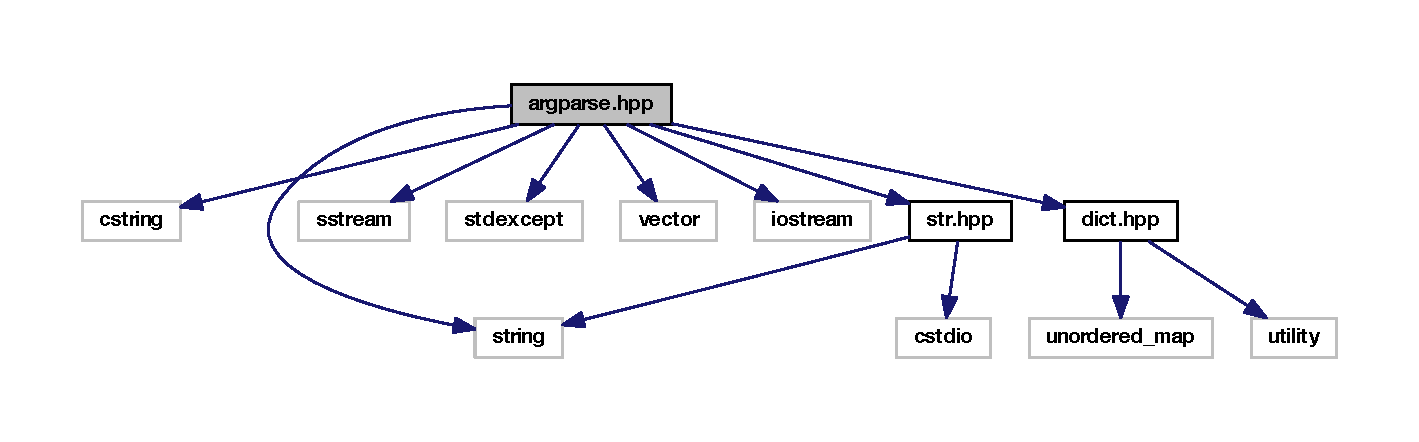
\includegraphics[width=350pt]{argparse_8hpp__incl}
\end{center}
\end{figure}
This graph shows which files directly or indirectly include this file\-:\nopagebreak
\begin{figure}[H]
\begin{center}
\leavevmode
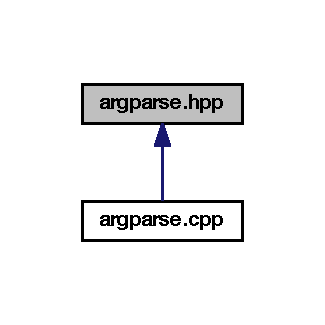
\includegraphics[width=156pt]{argparse_8hpp__dep__incl}
\end{center}
\end{figure}
\subsection*{Classes}
\begin{DoxyCompactItemize}
\item 
struct \hyperlink{structargparse_1_1_arg_holder}{argparse\-::\-Arg\-Holder}
\begin{DoxyCompactList}\small\item\em Holds the result of parsing arguments. \end{DoxyCompactList}\end{DoxyCompactItemize}
\subsection*{Namespaces}
\begin{DoxyCompactItemize}
\item 
namespace \hyperlink{namespaceargparse}{argparse}
\begin{DoxyCompactList}\small\item\em Command-\/line argument parser with a focus on brevity. \end{DoxyCompactList}\end{DoxyCompactItemize}
\subsection*{Functions}
\begin{DoxyCompactItemize}
\item 
string \hyperlink{namespaceargparse_a0ee3e8ca883816181b45c15a9ad0b6ed}{argparse\-::make\-Usage\-String} (const string \&prog\-Name, const string \&desc, const string \&pos\-Args=string(), const dict\-::\-Dict$<$ string, string $>$ \&opt\-To\-Help=dict\-::\-Dict$<$ string, string $>$(), unsigned cols=80, unsigned help\-Cols=60)
\begin{DoxyCompactList}\small\item\em Create a usage string. \end{DoxyCompactList}\item 
{\footnotesize template$<$class Func\-Type $>$ }\\Arg\-Holder \hyperlink{namespaceargparse_a4b1b6c03b45175acd13d1620f328e4aa}{argparse\-::parse} (int argc, const char $\ast$argv\mbox{[}$\,$\mbox{]}, const dict\-::\-Dict$<$ string, Func\-Type $>$ \&opt\-To\-Chker, char opt\-Char='-\/', bool gen\-Help\-Chker=true)
\begin{DoxyCompactList}\small\item\em Return an \hyperlink{structargparse_1_1_arg_holder}{Arg\-Holder} object holding the parsed arguments. \end{DoxyCompactList}\item 
\hyperlink{structargparse_1_1_arg_holder}{Arg\-Holder} \hyperlink{namespaceargparse_a6cfba06102a610840779069dfda1b98d}{argparse\-::parse} (int argc, const char $\ast$argv\mbox{[}$\,$\mbox{]}, const char opt\-Char='-\/', bool gen\-Help\-Chker=true)
\begin{DoxyCompactList}\small\item\em For programs that take no options. \end{DoxyCompactList}\end{DoxyCompactItemize}

\hypertarget{autodiff_8cpp}{\section{autodiff.\-cpp File Reference}
\label{autodiff_8cpp}\index{autodiff.\-cpp@{autodiff.\-cpp}}
}
{\ttfamily \#include $<$cmath$>$}\\*
{\ttfamily \#include $<$iostream$>$}\\*
{\ttfamily \#include \char`\"{}autodiff.\-hpp\char`\"{}}\\*
Include dependency graph for autodiff.\-cpp\-:\nopagebreak
\begin{figure}[H]
\begin{center}
\leavevmode
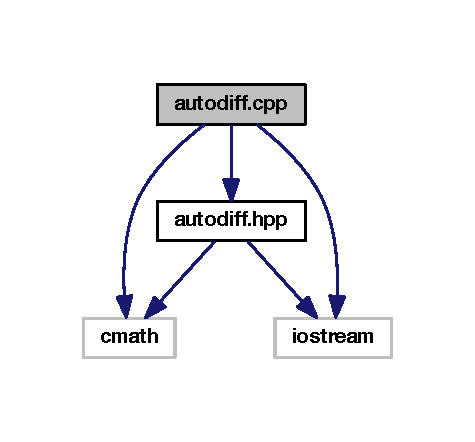
\includegraphics[width=228pt]{autodiff_8cpp__incl}
\end{center}
\end{figure}
\subsection*{Functions}
\begin{DoxyCompactItemize}
\item 
\hyperlink{structautodiff_1_1_dual_num}{Dual\-Num} \hyperlink{autodiff_8cpp_ae633308d2e5c4d2d185d53392e5b5b0a}{operator+} (const \hyperlink{structautodiff_1_1_dual_num}{Dual\-Num} \&a, const \hyperlink{structautodiff_1_1_dual_num}{Dual\-Num} \&b)
\item 
\hyperlink{structautodiff_1_1_dual_num}{Dual\-Num} \hyperlink{autodiff_8cpp_a787adac37341401ca38bde2c1825bf81}{operator-\/} (const \hyperlink{structautodiff_1_1_dual_num}{Dual\-Num} \&a, const \hyperlink{structautodiff_1_1_dual_num}{Dual\-Num} \&b)
\item 
\hyperlink{structautodiff_1_1_dual_num}{Dual\-Num} \hyperlink{autodiff_8cpp_a60637211a905130baeea07ba82cae9be}{operator-\/} (const \hyperlink{structautodiff_1_1_dual_num}{Dual\-Num} \&a)
\item 
\hyperlink{structautodiff_1_1_dual_num}{Dual\-Num} \hyperlink{autodiff_8cpp_a61d7fbca36cfb9a09a1726a2bfb82145}{operator$\ast$} (const \hyperlink{structautodiff_1_1_dual_num}{Dual\-Num} \&a, const \hyperlink{structautodiff_1_1_dual_num}{Dual\-Num} \&b)
\item 
\hyperlink{structautodiff_1_1_dual_num}{Dual\-Num} \hyperlink{autodiff_8cpp_a9726b843fee19d087ae7076cfe01ce12}{operator/} (const \hyperlink{structautodiff_1_1_dual_num}{Dual\-Num} \&a, const \hyperlink{structautodiff_1_1_dual_num}{Dual\-Num} \&b)
\item 
ostream \& \hyperlink{autodiff_8cpp_ab6b5f25da3be3e795c39283305527bb3}{operator$<$$<$} (ostream \&out, const \hyperlink{structautodiff_1_1_dual_num}{Dual\-Num} \&a)
\end{DoxyCompactItemize}


\subsection{Function Documentation}
\hypertarget{autodiff_8cpp_a61d7fbca36cfb9a09a1726a2bfb82145}{\index{autodiff.\-cpp@{autodiff.\-cpp}!operator$\ast$@{operator$\ast$}}
\index{operator$\ast$@{operator$\ast$}!autodiff.cpp@{autodiff.\-cpp}}
\subsubsection[{operator$\ast$}]{\setlength{\rightskip}{0pt plus 5cm}{\bf Dual\-Num} operator$\ast$ (
\begin{DoxyParamCaption}
\item[{const {\bf Dual\-Num} \&}]{a, }
\item[{const {\bf Dual\-Num} \&}]{b}
\end{DoxyParamCaption}
)}}\label{autodiff_8cpp_a61d7fbca36cfb9a09a1726a2bfb82145}
\hypertarget{autodiff_8cpp_ae633308d2e5c4d2d185d53392e5b5b0a}{\index{autodiff.\-cpp@{autodiff.\-cpp}!operator+@{operator+}}
\index{operator+@{operator+}!autodiff.cpp@{autodiff.\-cpp}}
\subsubsection[{operator+}]{\setlength{\rightskip}{0pt plus 5cm}{\bf Dual\-Num} operator+ (
\begin{DoxyParamCaption}
\item[{const {\bf Dual\-Num} \&}]{a, }
\item[{const {\bf Dual\-Num} \&}]{b}
\end{DoxyParamCaption}
)}}\label{autodiff_8cpp_ae633308d2e5c4d2d185d53392e5b5b0a}
\hypertarget{autodiff_8cpp_a787adac37341401ca38bde2c1825bf81}{\index{autodiff.\-cpp@{autodiff.\-cpp}!operator-\/@{operator-\/}}
\index{operator-\/@{operator-\/}!autodiff.cpp@{autodiff.\-cpp}}
\subsubsection[{operator-\/}]{\setlength{\rightskip}{0pt plus 5cm}{\bf Dual\-Num} operator-\/ (
\begin{DoxyParamCaption}
\item[{const {\bf Dual\-Num} \&}]{a, }
\item[{const {\bf Dual\-Num} \&}]{b}
\end{DoxyParamCaption}
)}}\label{autodiff_8cpp_a787adac37341401ca38bde2c1825bf81}
\hypertarget{autodiff_8cpp_a60637211a905130baeea07ba82cae9be}{\index{autodiff.\-cpp@{autodiff.\-cpp}!operator-\/@{operator-\/}}
\index{operator-\/@{operator-\/}!autodiff.cpp@{autodiff.\-cpp}}
\subsubsection[{operator-\/}]{\setlength{\rightskip}{0pt plus 5cm}{\bf Dual\-Num} operator-\/ (
\begin{DoxyParamCaption}
\item[{const {\bf Dual\-Num} \&}]{a}
\end{DoxyParamCaption}
)}}\label{autodiff_8cpp_a60637211a905130baeea07ba82cae9be}
\hypertarget{autodiff_8cpp_a9726b843fee19d087ae7076cfe01ce12}{\index{autodiff.\-cpp@{autodiff.\-cpp}!operator/@{operator/}}
\index{operator/@{operator/}!autodiff.cpp@{autodiff.\-cpp}}
\subsubsection[{operator/}]{\setlength{\rightskip}{0pt plus 5cm}{\bf Dual\-Num} operator/ (
\begin{DoxyParamCaption}
\item[{const {\bf Dual\-Num} \&}]{a, }
\item[{const {\bf Dual\-Num} \&}]{b}
\end{DoxyParamCaption}
)}}\label{autodiff_8cpp_a9726b843fee19d087ae7076cfe01ce12}
\hypertarget{autodiff_8cpp_ab6b5f25da3be3e795c39283305527bb3}{\index{autodiff.\-cpp@{autodiff.\-cpp}!operator$<$$<$@{operator$<$$<$}}
\index{operator$<$$<$@{operator$<$$<$}!autodiff.cpp@{autodiff.\-cpp}}
\subsubsection[{operator$<$$<$}]{\setlength{\rightskip}{0pt plus 5cm}ostream\& operator$<$$<$ (
\begin{DoxyParamCaption}
\item[{ostream \&}]{out, }
\item[{const {\bf Dual\-Num} \&}]{a}
\end{DoxyParamCaption}
)}}\label{autodiff_8cpp_ab6b5f25da3be3e795c39283305527bb3}

\hypertarget{autodiff_8hpp}{\section{autodiff.\-hpp File Reference}
\label{autodiff_8hpp}\index{autodiff.\-hpp@{autodiff.\-hpp}}
}
{\ttfamily \#include $<$cmath$>$}\\*
{\ttfamily \#include $<$iostream$>$}\\*
\subsection*{Classes}
\begin{DoxyCompactItemize}
\item 
struct \hyperlink{structautodiff_1_1_dual_num}{autodiff\-::\-Dual\-Num}
\begin{DoxyCompactList}\small\item\em Represents the \char`\"{}real\char`\"{} part of a number in member {\ttfamily r} and the derivative in {\ttfamily d}. \end{DoxyCompactList}\end{DoxyCompactItemize}
\subsection*{Namespaces}
\begin{DoxyCompactItemize}
\item 
namespace \hyperlink{namespaceautodiff}{autodiff}
\begin{DoxyCompactList}\small\item\em Implements automatic differentiation. \end{DoxyCompactList}\end{DoxyCompactItemize}
\subsection*{Functions}
\begin{DoxyCompactItemize}
\item 
\hyperlink{structautodiff_1_1_dual_num}{Dual\-Num} \hyperlink{namespaceautodiff_a19b889e35f523cc6ca0f377dc8bed262}{autodiff\-::d\-Pow} (const \hyperlink{structautodiff_1_1_dual_num}{Dual\-Num} \&a, const \hyperlink{structautodiff_1_1_dual_num}{Dual\-Num} \&b)
\item 
\hyperlink{structautodiff_1_1_dual_num}{Dual\-Num} \hyperlink{namespaceautodiff_a0f6df25515f7f05f838a9fd96f53fd37}{autodiff\-::d\-Sin} (const \hyperlink{structautodiff_1_1_dual_num}{Dual\-Num} \&a)
\item 
\hyperlink{structautodiff_1_1_dual_num}{Dual\-Num} \hyperlink{namespaceautodiff_a49d66a6f54fffb4250795cc589158a14}{autodiff\-::d\-Cos} (const \hyperlink{structautodiff_1_1_dual_num}{Dual\-Num} \&a)
\item 
\hyperlink{structautodiff_1_1_dual_num}{Dual\-Num} \hyperlink{namespaceautodiff_a4bdb0754d9ad8a5c4aba2d7ea9f040db}{autodiff\-::d\-Tan} (const \hyperlink{structautodiff_1_1_dual_num}{Dual\-Num} \&a)
\item 
\hyperlink{structautodiff_1_1_dual_num}{Dual\-Num} \hyperlink{namespaceautodiff_af2706967e031d3472b823760b0c67dcb}{autodiff\-::d\-Exp} (const \hyperlink{structautodiff_1_1_dual_num}{Dual\-Num} \&a)
\item 
\hyperlink{structautodiff_1_1_dual_num}{Dual\-Num} \hyperlink{namespaceautodiff_a003e7455b4727bad71fdb9b6bc676e86}{autodiff\-::d\-Log} (const \hyperlink{structautodiff_1_1_dual_num}{Dual\-Num} \&a)
\item 
\hyperlink{structautodiff_1_1_dual_num}{Dual\-Num} \hyperlink{namespaceautodiff_a656dafc1fc9422d40ade97d24905f875}{autodiff\-::d\-Log10} (const \hyperlink{structautodiff_1_1_dual_num}{Dual\-Num} \&a)
\item 
\hyperlink{structautodiff_1_1_dual_num}{autodiff\-::\-Dual\-Num} \hyperlink{autodiff_8hpp_afcaa49648f532c1593415c845c2fdba6}{operator+} (const \hyperlink{structautodiff_1_1_dual_num}{autodiff\-::\-Dual\-Num} \&a, const \hyperlink{structautodiff_1_1_dual_num}{autodiff\-::\-Dual\-Num} \&b)
\item 
\hyperlink{structautodiff_1_1_dual_num}{autodiff\-::\-Dual\-Num} \hyperlink{autodiff_8hpp_a74872447d0a3ced20978ab51ee1f657d}{operator-\/} (const \hyperlink{structautodiff_1_1_dual_num}{autodiff\-::\-Dual\-Num} \&a, const \hyperlink{structautodiff_1_1_dual_num}{autodiff\-::\-Dual\-Num} \&b)
\item 
\hyperlink{structautodiff_1_1_dual_num}{autodiff\-::\-Dual\-Num} \hyperlink{autodiff_8hpp_a5b2488b390f5cf4f33ba2d057209eace}{operator-\/} (const \hyperlink{structautodiff_1_1_dual_num}{autodiff\-::\-Dual\-Num} \&a)
\item 
\hyperlink{structautodiff_1_1_dual_num}{autodiff\-::\-Dual\-Num} \hyperlink{autodiff_8hpp_a87030a560abe7446ab81995b3724cc51}{operator$\ast$} (const \hyperlink{structautodiff_1_1_dual_num}{autodiff\-::\-Dual\-Num} \&a, const \hyperlink{structautodiff_1_1_dual_num}{autodiff\-::\-Dual\-Num} \&b)
\item 
\hyperlink{structautodiff_1_1_dual_num}{autodiff\-::\-Dual\-Num} \hyperlink{autodiff_8hpp_a0fa02b284f6ac59a838b8458d2dc381b}{operator/} (const \hyperlink{structautodiff_1_1_dual_num}{autodiff\-::\-Dual\-Num} \&a, const \hyperlink{structautodiff_1_1_dual_num}{autodiff\-::\-Dual\-Num} \&b)
\item 
ostream \& \hyperlink{autodiff_8hpp_aba8d3eb9946f938d7ea0f6980732bfb5}{operator$<$$<$} (ostream \&out, const \hyperlink{structautodiff_1_1_dual_num}{autodiff\-::\-Dual\-Num} \&a)
\end{DoxyCompactItemize}
\subsection*{Variables}
\begin{DoxyCompactItemize}
\item 
const double \hyperlink{namespaceautodiff_ac438d71cd4847e9f19efe6a4f1cfd5d7}{autodiff\-::\-I\-N\-V\-\_\-\-L\-O\-G\-\_\-10} = 1 / log(10)
\end{DoxyCompactItemize}


\subsection{Function Documentation}
\hypertarget{autodiff_8hpp_a87030a560abe7446ab81995b3724cc51}{\index{autodiff.\-hpp@{autodiff.\-hpp}!operator$\ast$@{operator$\ast$}}
\index{operator$\ast$@{operator$\ast$}!autodiff.hpp@{autodiff.\-hpp}}
\subsubsection[{operator$\ast$}]{\setlength{\rightskip}{0pt plus 5cm}{\bf autodiff\-::\-Dual\-Num} operator$\ast$ (
\begin{DoxyParamCaption}
\item[{const {\bf autodiff\-::\-Dual\-Num} \&}]{a, }
\item[{const {\bf autodiff\-::\-Dual\-Num} \&}]{b}
\end{DoxyParamCaption}
)}}\label{autodiff_8hpp_a87030a560abe7446ab81995b3724cc51}
\hypertarget{autodiff_8hpp_afcaa49648f532c1593415c845c2fdba6}{\index{autodiff.\-hpp@{autodiff.\-hpp}!operator+@{operator+}}
\index{operator+@{operator+}!autodiff.hpp@{autodiff.\-hpp}}
\subsubsection[{operator+}]{\setlength{\rightskip}{0pt plus 5cm}{\bf autodiff\-::\-Dual\-Num} operator+ (
\begin{DoxyParamCaption}
\item[{const {\bf autodiff\-::\-Dual\-Num} \&}]{a, }
\item[{const {\bf autodiff\-::\-Dual\-Num} \&}]{b}
\end{DoxyParamCaption}
)}}\label{autodiff_8hpp_afcaa49648f532c1593415c845c2fdba6}
\hypertarget{autodiff_8hpp_a74872447d0a3ced20978ab51ee1f657d}{\index{autodiff.\-hpp@{autodiff.\-hpp}!operator-\/@{operator-\/}}
\index{operator-\/@{operator-\/}!autodiff.hpp@{autodiff.\-hpp}}
\subsubsection[{operator-\/}]{\setlength{\rightskip}{0pt plus 5cm}{\bf autodiff\-::\-Dual\-Num} operator-\/ (
\begin{DoxyParamCaption}
\item[{const {\bf autodiff\-::\-Dual\-Num} \&}]{a, }
\item[{const {\bf autodiff\-::\-Dual\-Num} \&}]{b}
\end{DoxyParamCaption}
)}}\label{autodiff_8hpp_a74872447d0a3ced20978ab51ee1f657d}
\hypertarget{autodiff_8hpp_a5b2488b390f5cf4f33ba2d057209eace}{\index{autodiff.\-hpp@{autodiff.\-hpp}!operator-\/@{operator-\/}}
\index{operator-\/@{operator-\/}!autodiff.hpp@{autodiff.\-hpp}}
\subsubsection[{operator-\/}]{\setlength{\rightskip}{0pt plus 5cm}{\bf autodiff\-::\-Dual\-Num} operator-\/ (
\begin{DoxyParamCaption}
\item[{const {\bf autodiff\-::\-Dual\-Num} \&}]{a}
\end{DoxyParamCaption}
)}}\label{autodiff_8hpp_a5b2488b390f5cf4f33ba2d057209eace}
\hypertarget{autodiff_8hpp_a0fa02b284f6ac59a838b8458d2dc381b}{\index{autodiff.\-hpp@{autodiff.\-hpp}!operator/@{operator/}}
\index{operator/@{operator/}!autodiff.hpp@{autodiff.\-hpp}}
\subsubsection[{operator/}]{\setlength{\rightskip}{0pt plus 5cm}{\bf autodiff\-::\-Dual\-Num} operator/ (
\begin{DoxyParamCaption}
\item[{const {\bf autodiff\-::\-Dual\-Num} \&}]{a, }
\item[{const {\bf autodiff\-::\-Dual\-Num} \&}]{b}
\end{DoxyParamCaption}
)}}\label{autodiff_8hpp_a0fa02b284f6ac59a838b8458d2dc381b}
\hypertarget{autodiff_8hpp_aba8d3eb9946f938d7ea0f6980732bfb5}{\index{autodiff.\-hpp@{autodiff.\-hpp}!operator$<$$<$@{operator$<$$<$}}
\index{operator$<$$<$@{operator$<$$<$}!autodiff.hpp@{autodiff.\-hpp}}
\subsubsection[{operator$<$$<$}]{\setlength{\rightskip}{0pt plus 5cm}ostream\& operator$<$$<$ (
\begin{DoxyParamCaption}
\item[{ostream \&}]{out, }
\item[{const {\bf autodiff\-::\-Dual\-Num} \&}]{a}
\end{DoxyParamCaption}
)}}\label{autodiff_8hpp_aba8d3eb9946f938d7ea0f6980732bfb5}

\hypertarget{cvutils_8cpp}{\section{cvutils.\-cpp File Reference}
\label{cvutils_8cpp}\index{cvutils.\-cpp@{cvutils.\-cpp}}
}
{\ttfamily \#include $<$cstdint$>$}\\*
{\ttfamily \#include $<$algorithm$>$}\\*
{\ttfamily \#include $<$iostream$>$}\\*
{\ttfamily \#include $<$opencv2/opencv.\-hpp$>$}\\*
{\ttfamily \#include \char`\"{}cvutils.\-hpp\char`\"{}}\\*
{\ttfamily \#include \char`\"{}kmath.\-hpp\char`\"{}}\\*
Include dependency graph for cvutils.\-cpp\-:
\nopagebreak
\begin{figure}[H]
\begin{center}
\leavevmode
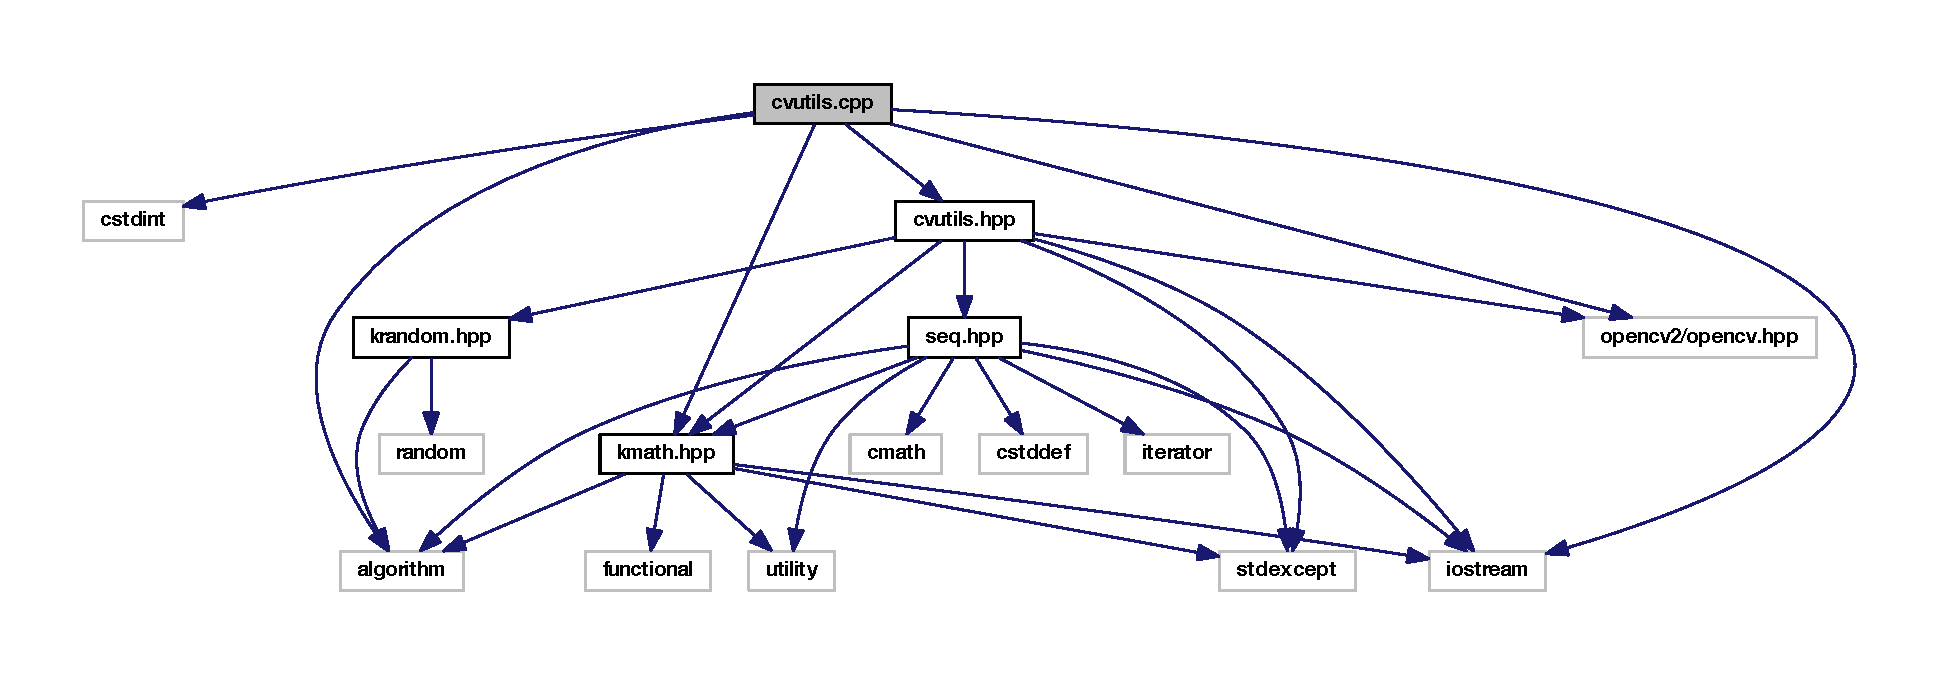
\includegraphics[width=350pt]{cvutils_8cpp__incl}
\end{center}
\end{figure}
\subsection*{Functions}
\begin{DoxyCompactItemize}
\item 
ostream \& \hyperlink{cvutils_8cpp_a8e51a09bac9db8fc1086987161a5cde6}{operator$<$$<$} (ostream \&out, const Rect r)
\item 
ostream \& \hyperlink{cvutils_8cpp_a40e1aedcd73028caaf91a9799864d28b}{operator$<$$<$} (ostream \&out, const Size s)
\item 
ostream \& \hyperlink{cvutils_8cpp_ad24b7492cab7eddd53c2c12e61b21f13}{operator$<$$<$} (ostream \&out, const Size2f s)
\item 
ostream \& \hyperlink{cvutils_8cpp_aeaadaf0340a8cbab0ebe95c6d838e3d5}{operator$<$$<$} (ostream \&out, const Scalar s)
\item 
ostream \& \hyperlink{cvutils_8cpp_a19e2583b33817fa0157b7ba5d0ef42cb}{operator$<$$<$} (ostream \&out, const uchar c)
\item 
Size2f \hyperlink{cvutils_8cpp_ae180673a678e0c21b86f8c289c096c9a}{operator$\ast$} (const Size2f \&s, float a)
\item 
Size2f \hyperlink{cvutils_8cpp_aa0e8d1466faa50fc2e5d39500a83f3ad}{operator$\ast$} (float a, const Size2f \&s)
\item 
Size2f \hyperlink{cvutils_8cpp_aa6299a78aae948a9d8a8f5dfbc8c1305}{operator/} (const Size2f \&s, float a)
\item 
bool \hyperlink{cvutils_8cpp_a1d6da8c1cf5d528e8eeaefcc12e7ab85}{operator==} (const Size2f \&a, const Size2f \&b)
\item 
bool \hyperlink{cvutils_8cpp_acff1ba895a3cb7b31c791335098eca94}{operator!=} (const Size2f \&a, const Size2f \&b)
\end{DoxyCompactItemize}


\subsection{Function Documentation}
\hypertarget{cvutils_8cpp_a8e51a09bac9db8fc1086987161a5cde6}{\index{cvutils.\-cpp@{cvutils.\-cpp}!operator$<$$<$@{operator$<$$<$}}
\index{operator$<$$<$@{operator$<$$<$}!cvutils.cpp@{cvutils.\-cpp}}
\subsubsection[{operator$<$$<$}]{\setlength{\rightskip}{0pt plus 5cm}ostream\& operator$<$$<$ (
\begin{DoxyParamCaption}
\item[{ostream \&}]{out, }
\item[{const Rect}]{r}
\end{DoxyParamCaption}
)}}\label{cvutils_8cpp_a8e51a09bac9db8fc1086987161a5cde6}
\hypertarget{cvutils_8cpp_a40e1aedcd73028caaf91a9799864d28b}{\index{cvutils.\-cpp@{cvutils.\-cpp}!operator$<$$<$@{operator$<$$<$}}
\index{operator$<$$<$@{operator$<$$<$}!cvutils.cpp@{cvutils.\-cpp}}
\subsubsection[{operator$<$$<$}]{\setlength{\rightskip}{0pt plus 5cm}ostream\& operator$<$$<$ (
\begin{DoxyParamCaption}
\item[{ostream \&}]{out, }
\item[{const Size}]{s}
\end{DoxyParamCaption}
)}}\label{cvutils_8cpp_a40e1aedcd73028caaf91a9799864d28b}
\hypertarget{cvutils_8cpp_ad24b7492cab7eddd53c2c12e61b21f13}{\index{cvutils.\-cpp@{cvutils.\-cpp}!operator$<$$<$@{operator$<$$<$}}
\index{operator$<$$<$@{operator$<$$<$}!cvutils.cpp@{cvutils.\-cpp}}
\subsubsection[{operator$<$$<$}]{\setlength{\rightskip}{0pt plus 5cm}ostream\& operator$<$$<$ (
\begin{DoxyParamCaption}
\item[{ostream \&}]{out, }
\item[{const Size2f}]{s}
\end{DoxyParamCaption}
)}}\label{cvutils_8cpp_ad24b7492cab7eddd53c2c12e61b21f13}
\hypertarget{cvutils_8cpp_aeaadaf0340a8cbab0ebe95c6d838e3d5}{\index{cvutils.\-cpp@{cvutils.\-cpp}!operator$<$$<$@{operator$<$$<$}}
\index{operator$<$$<$@{operator$<$$<$}!cvutils.cpp@{cvutils.\-cpp}}
\subsubsection[{operator$<$$<$}]{\setlength{\rightskip}{0pt plus 5cm}ostream\& operator$<$$<$ (
\begin{DoxyParamCaption}
\item[{ostream \&}]{out, }
\item[{const Scalar}]{s}
\end{DoxyParamCaption}
)}}\label{cvutils_8cpp_aeaadaf0340a8cbab0ebe95c6d838e3d5}
\hypertarget{cvutils_8cpp_a19e2583b33817fa0157b7ba5d0ef42cb}{\index{cvutils.\-cpp@{cvutils.\-cpp}!operator$<$$<$@{operator$<$$<$}}
\index{operator$<$$<$@{operator$<$$<$}!cvutils.cpp@{cvutils.\-cpp}}
\subsubsection[{operator$<$$<$}]{\setlength{\rightskip}{0pt plus 5cm}ostream\& operator$<$$<$ (
\begin{DoxyParamCaption}
\item[{ostream \&}]{out, }
\item[{const uchar}]{c}
\end{DoxyParamCaption}
)}}\label{cvutils_8cpp_a19e2583b33817fa0157b7ba5d0ef42cb}
\hypertarget{cvutils_8cpp_ae180673a678e0c21b86f8c289c096c9a}{\index{cvutils.\-cpp@{cvutils.\-cpp}!operator$\ast$@{operator$\ast$}}
\index{operator$\ast$@{operator$\ast$}!cvutils.cpp@{cvutils.\-cpp}}
\subsubsection[{operator$\ast$}]{\setlength{\rightskip}{0pt plus 5cm}Size2f operator$\ast$ (
\begin{DoxyParamCaption}
\item[{const Size2f \&}]{s, }
\item[{float}]{a}
\end{DoxyParamCaption}
)}}\label{cvutils_8cpp_ae180673a678e0c21b86f8c289c096c9a}
\hypertarget{cvutils_8cpp_aa0e8d1466faa50fc2e5d39500a83f3ad}{\index{cvutils.\-cpp@{cvutils.\-cpp}!operator$\ast$@{operator$\ast$}}
\index{operator$\ast$@{operator$\ast$}!cvutils.cpp@{cvutils.\-cpp}}
\subsubsection[{operator$\ast$}]{\setlength{\rightskip}{0pt plus 5cm}Size2f operator$\ast$ (
\begin{DoxyParamCaption}
\item[{float}]{a, }
\item[{const Size2f \&}]{s}
\end{DoxyParamCaption}
)}}\label{cvutils_8cpp_aa0e8d1466faa50fc2e5d39500a83f3ad}
\hypertarget{cvutils_8cpp_aa6299a78aae948a9d8a8f5dfbc8c1305}{\index{cvutils.\-cpp@{cvutils.\-cpp}!operator/@{operator/}}
\index{operator/@{operator/}!cvutils.cpp@{cvutils.\-cpp}}
\subsubsection[{operator/}]{\setlength{\rightskip}{0pt plus 5cm}Size2f operator/ (
\begin{DoxyParamCaption}
\item[{const Size2f \&}]{s, }
\item[{float}]{a}
\end{DoxyParamCaption}
)}}\label{cvutils_8cpp_aa6299a78aae948a9d8a8f5dfbc8c1305}
\hypertarget{cvutils_8cpp_a1d6da8c1cf5d528e8eeaefcc12e7ab85}{\index{cvutils.\-cpp@{cvutils.\-cpp}!operator==@{operator==}}
\index{operator==@{operator==}!cvutils.cpp@{cvutils.\-cpp}}
\subsubsection[{operator==}]{\setlength{\rightskip}{0pt plus 5cm}bool operator== (
\begin{DoxyParamCaption}
\item[{const Size2f \&}]{a, }
\item[{const Size2f \&}]{b}
\end{DoxyParamCaption}
)}}\label{cvutils_8cpp_a1d6da8c1cf5d528e8eeaefcc12e7ab85}
\hypertarget{cvutils_8cpp_acff1ba895a3cb7b31c791335098eca94}{\index{cvutils.\-cpp@{cvutils.\-cpp}!operator!=@{operator!=}}
\index{operator!=@{operator!=}!cvutils.cpp@{cvutils.\-cpp}}
\subsubsection[{operator!=}]{\setlength{\rightskip}{0pt plus 5cm}bool operator!= (
\begin{DoxyParamCaption}
\item[{const Size2f \&}]{a, }
\item[{const Size2f \&}]{b}
\end{DoxyParamCaption}
)}}\label{cvutils_8cpp_acff1ba895a3cb7b31c791335098eca94}

\hypertarget{cvutils_8hpp}{\section{cvutils.\-hpp File Reference}
\label{cvutils_8hpp}\index{cvutils.\-hpp@{cvutils.\-hpp}}
}
{\ttfamily \#include $<$iostream$>$}\\*
{\ttfamily \#include $<$opencv2/opencv.\-hpp$>$}\\*
\subsection*{Classes}
\begin{DoxyCompactItemize}
\item 
struct \hyperlink{structcvutils_1_1___data_depth___fixed}{cvutils\-::\-\_\-\-Data\-Depth\-\_\-\-Fixed$<$ T $>$}
\item 
struct \hyperlink{structcvutils_1_1___data_depth___fixed_3_01uchar_01_4}{cvutils\-::\-\_\-\-Data\-Depth\-\_\-\-Fixed$<$ uchar $>$}
\end{DoxyCompactItemize}
\subsection*{Namespaces}
\begin{DoxyCompactItemize}
\item 
namespace \hyperlink{namespacecvutils}{cvutils}
\begin{DoxyCompactList}\small\item\em Open\-C\-V utilities. \end{DoxyCompactList}\end{DoxyCompactItemize}
\subsection*{Functions}
\begin{DoxyCompactItemize}
\item 
void \hyperlink{namespacecvutils_aa292da4b50c7692374fdde56afdd6baf}{cvutils\-::wait\-For\-Keypress} ()
\item 
ostream \& \hyperlink{cvutils_8hpp_a0b14696e4e43f7a2a1e707fa208b4ea6}{operator$<$$<$} (ostream \&out, const cv\-::\-Rect r)
\item 
ostream \& \hyperlink{cvutils_8hpp_acac9a564a7e46f10e2e1603edac9e540}{operator$<$$<$} (ostream \&out, const cv\-::\-Size s)
\item 
ostream \& \hyperlink{cvutils_8hpp_a5b3e75872c29d47c8c8fe2226927b511}{operator$<$$<$} (ostream \&out, const cv\-::\-Size2f s)
\item 
ostream \& \hyperlink{cvutils_8hpp_a4ca6efe2216f3d895e6de2a5cec34fc1}{operator$<$$<$} (ostream \&out, const cv\-::\-Scalar s)
\item 
ostream \& \hyperlink{cvutils_8hpp_a19e2583b33817fa0157b7ba5d0ef42cb}{operator$<$$<$} (ostream \&out, const uchar c)
\item 
{\footnotesize template$<$typename T , int cn$>$ }\\ostream \& \hyperlink{cvutils_8hpp_a2a8d9a7b33a01731771e3ef6a6fbfa7f}{operator$<$$<$} (ostream \&out, const cv\-::\-Vec$<$ T, cn $>$ v)
\end{DoxyCompactItemize}


\subsection{Function Documentation}
\hypertarget{cvutils_8hpp_a0b14696e4e43f7a2a1e707fa208b4ea6}{\index{cvutils.\-hpp@{cvutils.\-hpp}!operator$<$$<$@{operator$<$$<$}}
\index{operator$<$$<$@{operator$<$$<$}!cvutils.hpp@{cvutils.\-hpp}}
\subsubsection[{operator$<$$<$}]{\setlength{\rightskip}{0pt plus 5cm}ostream\& operator$<$$<$ (
\begin{DoxyParamCaption}
\item[{ostream \&}]{out, }
\item[{const cv\-::\-Rect}]{r}
\end{DoxyParamCaption}
)}}\label{cvutils_8hpp_a0b14696e4e43f7a2a1e707fa208b4ea6}
\hypertarget{cvutils_8hpp_acac9a564a7e46f10e2e1603edac9e540}{\index{cvutils.\-hpp@{cvutils.\-hpp}!operator$<$$<$@{operator$<$$<$}}
\index{operator$<$$<$@{operator$<$$<$}!cvutils.hpp@{cvutils.\-hpp}}
\subsubsection[{operator$<$$<$}]{\setlength{\rightskip}{0pt plus 5cm}ostream\& operator$<$$<$ (
\begin{DoxyParamCaption}
\item[{ostream \&}]{out, }
\item[{const cv\-::\-Size}]{s}
\end{DoxyParamCaption}
)}}\label{cvutils_8hpp_acac9a564a7e46f10e2e1603edac9e540}
\hypertarget{cvutils_8hpp_a5b3e75872c29d47c8c8fe2226927b511}{\index{cvutils.\-hpp@{cvutils.\-hpp}!operator$<$$<$@{operator$<$$<$}}
\index{operator$<$$<$@{operator$<$$<$}!cvutils.hpp@{cvutils.\-hpp}}
\subsubsection[{operator$<$$<$}]{\setlength{\rightskip}{0pt plus 5cm}ostream\& operator$<$$<$ (
\begin{DoxyParamCaption}
\item[{ostream \&}]{out, }
\item[{const cv\-::\-Size2f}]{s}
\end{DoxyParamCaption}
)}}\label{cvutils_8hpp_a5b3e75872c29d47c8c8fe2226927b511}
\hypertarget{cvutils_8hpp_a4ca6efe2216f3d895e6de2a5cec34fc1}{\index{cvutils.\-hpp@{cvutils.\-hpp}!operator$<$$<$@{operator$<$$<$}}
\index{operator$<$$<$@{operator$<$$<$}!cvutils.hpp@{cvutils.\-hpp}}
\subsubsection[{operator$<$$<$}]{\setlength{\rightskip}{0pt plus 5cm}ostream\& operator$<$$<$ (
\begin{DoxyParamCaption}
\item[{ostream \&}]{out, }
\item[{const cv\-::\-Scalar}]{s}
\end{DoxyParamCaption}
)}}\label{cvutils_8hpp_a4ca6efe2216f3d895e6de2a5cec34fc1}
\hypertarget{cvutils_8hpp_a19e2583b33817fa0157b7ba5d0ef42cb}{\index{cvutils.\-hpp@{cvutils.\-hpp}!operator$<$$<$@{operator$<$$<$}}
\index{operator$<$$<$@{operator$<$$<$}!cvutils.hpp@{cvutils.\-hpp}}
\subsubsection[{operator$<$$<$}]{\setlength{\rightskip}{0pt plus 5cm}ostream\& operator$<$$<$ (
\begin{DoxyParamCaption}
\item[{ostream \&}]{out, }
\item[{const uchar}]{c}
\end{DoxyParamCaption}
)}}\label{cvutils_8hpp_a19e2583b33817fa0157b7ba5d0ef42cb}
\hypertarget{cvutils_8hpp_a2a8d9a7b33a01731771e3ef6a6fbfa7f}{\index{cvutils.\-hpp@{cvutils.\-hpp}!operator$<$$<$@{operator$<$$<$}}
\index{operator$<$$<$@{operator$<$$<$}!cvutils.hpp@{cvutils.\-hpp}}
\subsubsection[{operator$<$$<$}]{\setlength{\rightskip}{0pt plus 5cm}template$<$typename T , int cn$>$ ostream\& operator$<$$<$ (
\begin{DoxyParamCaption}
\item[{ostream \&}]{out, }
\item[{const cv\-::\-Vec$<$ T, cn $>$}]{v}
\end{DoxyParamCaption}
)}}\label{cvutils_8hpp_a2a8d9a7b33a01731771e3ef6a6fbfa7f}

\hypertarget{dict_8hpp}{\section{dict.\-hpp File Reference}
\label{dict_8hpp}\index{dict.\-hpp@{dict.\-hpp}}
}
{\ttfamily \#include $<$unordered\-\_\-map$>$}\\*
{\ttfamily \#include $<$utility$>$}\\*
\subsection*{Namespaces}
\begin{DoxyCompactItemize}
\item 
namespace \hyperlink{namespacedict}{dict}
\begin{DoxyCompactList}\small\item\em Utilities for working with {\ttfamily Dict}s ({\ttfamily unordered\-\_\-map}s). \end{DoxyCompactList}\end{DoxyCompactItemize}
\subsection*{Functions}
\begin{DoxyCompactItemize}
\item 
{\footnotesize template$<$typename Key\-Type , typename Val\-Type $>$ }\\void \hyperlink{dict_8hpp_aad450cc243fecdc56252ec17b2c7f242}{\-\_\-make\-Dict\-I\-P} (Dict$<$ Key\-Type, Val\-Type $>$ \&d, Key\-Type key, Val\-Type val)
\item 
{\footnotesize template$<$typename Key\-Type , typename Val\-Type , typename... Args$>$ }\\void \hyperlink{dict_8hpp_a63c4edeb75c1a98c92321da3c0feb818}{\-\_\-make\-Dict\-I\-P} (Dict$<$ Key\-Type, Val\-Type $>$ \&d, Key\-Type key, Val\-Type val, Args...\-args)
\item 
{\footnotesize template$<$typename Key\-Type , typename Val\-Type , typename... Args$>$ }\\Dict$<$ Key\-Type, Val\-Type $>$ \hyperlink{dict_8hpp_acf532dcb9ac916d2ac99b609a3a2422d}{make\-Dict} (Key\-Type key, Val\-Type val, Args...\-args)
\item 
{\footnotesize template$<$typename Key\-Type , typename Val\-Type $>$ }\\Dict$<$ Key\-Type, Val\-Type $>$ \hyperlink{dict_8hpp_a952263572be8fc115fb88a93631e6fc3}{make\-Dict} ()
\item 
{\footnotesize template$<$typename Key\-T , typename Val\-T $>$ }\\ostream \& \hyperlink{dict_8hpp_a3c4515d6a24ee85ca1ff76eff687c06b}{operator$<$$<$} (ostream \&out, const Dict$<$ Key\-T, Val\-T $>$ \&seq)
\item 
{\footnotesize template$<$typename Iter\-T , typename Elem\-T $>$ }\\Dict$<$ Elem\-T, unsigned $>$ \& \hyperlink{namespacedict_a25d4adabc11b7754dad27d591de51df6}{dict\-::count\-Elems} (const Iter\-T \&start, const Iter\-T \&end, Dict$<$ Elem\-T, unsigned $>$ \&out)
\end{DoxyCompactItemize}


\subsection{Function Documentation}
\hypertarget{dict_8hpp_aad450cc243fecdc56252ec17b2c7f242}{\index{dict.\-hpp@{dict.\-hpp}!\-\_\-make\-Dict\-I\-P@{\-\_\-make\-Dict\-I\-P}}
\index{\-\_\-make\-Dict\-I\-P@{\-\_\-make\-Dict\-I\-P}!dict.hpp@{dict.\-hpp}}
\subsubsection[{\-\_\-make\-Dict\-I\-P}]{\setlength{\rightskip}{0pt plus 5cm}template$<$typename Key\-Type , typename Val\-Type $>$ void {\bf \-\_\-make\-Dict\-I\-P} (
\begin{DoxyParamCaption}
\item[{Dict$<$ Key\-Type, Val\-Type $>$ \&}]{d, }
\item[{Key\-Type}]{key, }
\item[{Val\-Type}]{val}
\end{DoxyParamCaption}
)}}\label{dict_8hpp_aad450cc243fecdc56252ec17b2c7f242}
\hypertarget{dict_8hpp_a63c4edeb75c1a98c92321da3c0feb818}{\index{dict.\-hpp@{dict.\-hpp}!\-\_\-make\-Dict\-I\-P@{\-\_\-make\-Dict\-I\-P}}
\index{\-\_\-make\-Dict\-I\-P@{\-\_\-make\-Dict\-I\-P}!dict.hpp@{dict.\-hpp}}
\subsubsection[{\-\_\-make\-Dict\-I\-P}]{\setlength{\rightskip}{0pt plus 5cm}template$<$typename Key\-Type , typename Val\-Type , typename... Args$>$ void {\bf \-\_\-make\-Dict\-I\-P} (
\begin{DoxyParamCaption}
\item[{Dict$<$ Key\-Type, Val\-Type $>$ \&}]{d, }
\item[{Key\-Type}]{key, }
\item[{Val\-Type}]{val, }
\item[{Args...}]{args}
\end{DoxyParamCaption}
)}}\label{dict_8hpp_a63c4edeb75c1a98c92321da3c0feb818}
\hypertarget{dict_8hpp_acf532dcb9ac916d2ac99b609a3a2422d}{\index{dict.\-hpp@{dict.\-hpp}!make\-Dict@{make\-Dict}}
\index{make\-Dict@{make\-Dict}!dict.hpp@{dict.\-hpp}}
\subsubsection[{make\-Dict}]{\setlength{\rightskip}{0pt plus 5cm}template$<$typename Key\-Type , typename Val\-Type , typename... Args$>$ Dict$<$Key\-Type, Val\-Type$>$ {\bf make\-Dict} (
\begin{DoxyParamCaption}
\item[{Key\-Type}]{key, }
\item[{Val\-Type}]{val, }
\item[{Args...}]{args}
\end{DoxyParamCaption}
)}}\label{dict_8hpp_acf532dcb9ac916d2ac99b609a3a2422d}
\hypertarget{dict_8hpp_a952263572be8fc115fb88a93631e6fc3}{\index{dict.\-hpp@{dict.\-hpp}!make\-Dict@{make\-Dict}}
\index{make\-Dict@{make\-Dict}!dict.hpp@{dict.\-hpp}}
\subsubsection[{make\-Dict}]{\setlength{\rightskip}{0pt plus 5cm}template$<$typename Key\-Type , typename Val\-Type $>$ Dict$<$Key\-Type, Val\-Type$>$ {\bf make\-Dict} (
\begin{DoxyParamCaption}
{}
\end{DoxyParamCaption}
)}}\label{dict_8hpp_a952263572be8fc115fb88a93631e6fc3}
Construct a {\ttfamily Dict} ({\ttfamily unordered\-\_\-map}). For an empty {\ttfamily Dict}, must specify {\ttfamily Key\-Type} and {\ttfamily Val\-Type}. \hypertarget{dict_8hpp_a3c4515d6a24ee85ca1ff76eff687c06b}{\index{dict.\-hpp@{dict.\-hpp}!operator$<$$<$@{operator$<$$<$}}
\index{operator$<$$<$@{operator$<$$<$}!dict.hpp@{dict.\-hpp}}
\subsubsection[{operator$<$$<$}]{\setlength{\rightskip}{0pt plus 5cm}template$<$typename Key\-T , typename Val\-T $>$ ostream\& operator$<$$<$ (
\begin{DoxyParamCaption}
\item[{ostream \&}]{out, }
\item[{const Dict$<$ Key\-T, Val\-T $>$ \&}]{seq}
\end{DoxyParamCaption}
)}}\label{dict_8hpp_a3c4515d6a24ee85ca1ff76eff687c06b}
Print each element of a {\ttfamily Dict}. 
\hypertarget{io_8hpp}{\section{io.\-hpp File Reference}
\label{io_8hpp}\index{io.\-hpp@{io.\-hpp}}
}
{\ttfamily \#include $<$iostream$>$}\\*
Include dependency graph for io.\-hpp\-:
\nopagebreak
\begin{figure}[H]
\begin{center}
\leavevmode
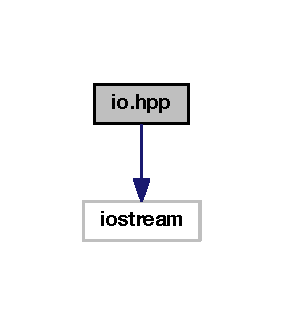
\includegraphics[width=136pt]{io_8hpp__incl}
\end{center}
\end{figure}
This graph shows which files directly or indirectly include this file\-:
\nopagebreak
\begin{figure}[H]
\begin{center}
\leavevmode
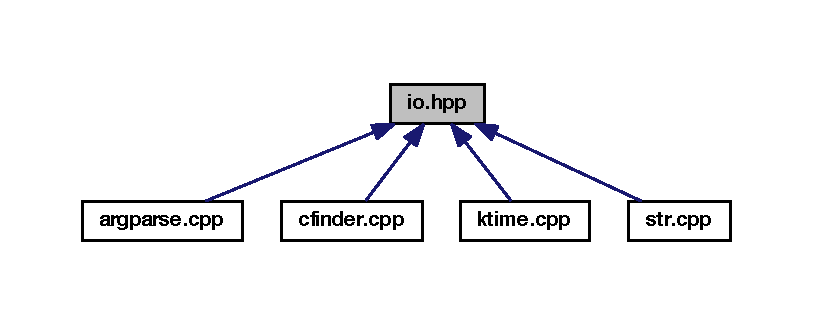
\includegraphics[width=350pt]{io_8hpp__dep__incl}
\end{center}
\end{figure}
\subsection*{Namespaces}
\begin{DoxyCompactItemize}
\item 
namespace \hyperlink{namespaceio}{io}
\begin{DoxyCompactList}\small\item\em Convenience functions for printing values. \end{DoxyCompactList}\end{DoxyCompactItemize}
\subsection*{Functions}
\begin{DoxyCompactItemize}
\item 
{\footnotesize template$<$typename T1 , typename T2 $>$ }\\ostream \& \hyperlink{io_8hpp_a932f5ab08815fcdc72f2866b0d6e1ee2}{operator$<$$<$} (ostream \&out, const pair$<$ T1, T2 $>$ \&p)
\begin{DoxyCompactList}\small\item\em Print a {\ttfamily pair}. \end{DoxyCompactList}\item 
void \hyperlink{namespaceio_ad8499487f5202220fead59833138f4ab}{io\-::print} ()
\begin{DoxyCompactList}\small\item\em Simply print a newline. \end{DoxyCompactList}\item 
{\footnotesize template$<$typename T , typename... Args$>$ }\\void \hyperlink{namespaceio_ab9528b2fe57a002bb153f1b9f8dde743}{io\-::print} (T value, Args...\-args)
\begin{DoxyCompactList}\small\item\em Print arguments separated by spaces, then a newline. \end{DoxyCompactList}\item 
void \hyperlink{namespaceio_ae85db8edfd95c17427c2606360bb97af}{io\-::print\-Imm} ()
\begin{DoxyCompactList}\small\item\em Call {\ttfamily fflush(stdout);}. \end{DoxyCompactList}\item 
{\footnotesize template$<$typename T , typename... Args$>$ }\\void \hyperlink{namespaceio_ade4f05edb2cd007404540f67d416bd4a}{io\-::print\-Imm} (T value, Args...\-args)
\begin{DoxyCompactList}\small\item\em Print arguments separated by spaces with no newline (by default values only show up on the screen when a newline is printed). \end{DoxyCompactList}\end{DoxyCompactItemize}


\subsection{Function Documentation}
\hypertarget{io_8hpp_a932f5ab08815fcdc72f2866b0d6e1ee2}{\index{io.\-hpp@{io.\-hpp}!operator$<$$<$@{operator$<$$<$}}
\index{operator$<$$<$@{operator$<$$<$}!io.hpp@{io.\-hpp}}
\subsubsection[{operator$<$$<$}]{\setlength{\rightskip}{0pt plus 5cm}template$<$typename T1 , typename T2 $>$ ostream\& operator$<$$<$ (
\begin{DoxyParamCaption}
\item[{ostream \&}]{out, }
\item[{const pair$<$ T1, T2 $>$ \&}]{p}
\end{DoxyParamCaption}
)}}\label{io_8hpp_a932f5ab08815fcdc72f2866b0d6e1ee2}


Print a {\ttfamily pair}. 


\hypertarget{krandom_8cpp}{\section{krandom.\-cpp File Reference}
\label{krandom_8cpp}\index{krandom.\-cpp@{krandom.\-cpp}}
}
{\ttfamily \#include $<$random$>$}\\*
{\ttfamily \#include \char`\"{}krandom.\-hpp\char`\"{}}\\*
Include dependency graph for krandom.\-cpp\-:
\nopagebreak
\begin{figure}[H]
\begin{center}
\leavevmode
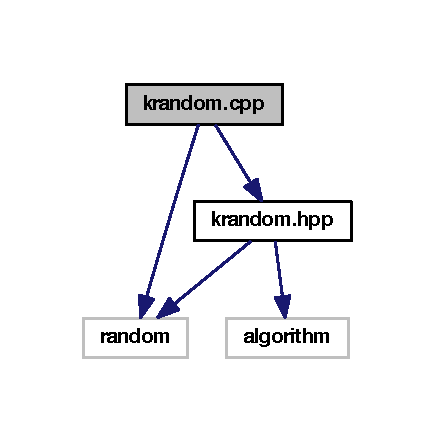
\includegraphics[width=208pt]{krandom_8cpp__incl}
\end{center}
\end{figure}
\subsection*{Functions}
\begin{DoxyCompactItemize}
\item 
vector$<$ unsigned $>$ \hyperlink{krandom_8cpp_a55dd773165033113e7e200186d6e88ad}{get\-Sample\-Inds} (unsigned pop\-Size, unsigned samp\-Size, bool with\-Replacement)
\end{DoxyCompactItemize}


\subsection{Function Documentation}
\hypertarget{krandom_8cpp_a55dd773165033113e7e200186d6e88ad}{\index{krandom.\-cpp@{krandom.\-cpp}!get\-Sample\-Inds@{get\-Sample\-Inds}}
\index{get\-Sample\-Inds@{get\-Sample\-Inds}!krandom.cpp@{krandom.\-cpp}}
\subsubsection[{get\-Sample\-Inds}]{\setlength{\rightskip}{0pt plus 5cm}vector$<$unsigned$>$ {\bf get\-Sample\-Inds} (
\begin{DoxyParamCaption}
\item[{unsigned}]{pop\-Size, }
\item[{unsigned}]{samp\-Size, }
\item[{bool}]{with\-Replacement}
\end{DoxyParamCaption}
)}}\label{krandom_8cpp_a55dd773165033113e7e200186d6e88ad}

\hypertarget{krandom_8hpp}{\section{krandom.\-hpp File Reference}
\label{krandom_8hpp}\index{krandom.\-hpp@{krandom.\-hpp}}
}
{\ttfamily \#include $<$random$>$}\\*
{\ttfamily \#include $<$algorithm$>$}\\*
\subsection*{Namespaces}
\begin{DoxyCompactItemize}
\item 
namespace \hyperlink{namespacekrandom}{krandom}
\begin{DoxyCompactList}\small\item\em Simple wrapper around {\ttfamily $<$random$>$} with a Python interface. \end{DoxyCompactList}\end{DoxyCompactItemize}
\subsection*{Functions}
\begin{DoxyCompactItemize}
\item 
int \hyperlink{namespacekrandom_a32b7337c1131ea0fbbd6b5f20aac2002}{krandom\-::randint} (int low, int high)
\item 
long \hyperlink{namespacekrandom_adc8e2bfa37c40fdecc8f601a266ab447}{krandom\-::randint} (long low, long high)
\item 
long long \hyperlink{namespacekrandom_a4672262133b6b130d7ca8b49f55595a2}{krandom\-::randint} (long long low, long long high)
\item 
double \hyperlink{namespacekrandom_a6a320147afafc7e81429b1a1ab4ec2e0}{krandom\-::random} ()
\item 
float \hyperlink{namespacekrandom_aa5f77704c3bf39731c986b7d27caf0fe}{krandom\-::uniform} (float low, float high)
\item 
double \hyperlink{namespacekrandom_ae89a756b3d067650aa9712efe6e930e2}{krandom\-::uniform} (double low, double high)
\item 
{\footnotesize template$<$class Iter\-Type $>$ }\\void \hyperlink{namespacekrandom_abac374525fd029faa58cb9c43cab41eb}{krandom\-::shuffle} (Iter\-Type start, Iter\-Type end)
\item 
{\footnotesize template$<$class Seq\-Type $>$ }\\void \hyperlink{namespacekrandom_a3cf920703fa6e180b1aa4d4c86799626}{krandom\-::shuffle} (Seq\-Type \&seq)
\item 
{\footnotesize template$<$template$<$ typename U, typename...\-Args $>$ class Seq\-Type, typename Item\-Type $>$ }\\Item\-Type \hyperlink{namespacekrandom_a59c038687d5825d1b6b8f26cf91dee20}{krandom\-::choice} (const Seq\-Type$<$ Item\-Type $>$ \&seq)
\item 
vector$<$ unsigned $>$ \& \hyperlink{namespacekrandom_a50015c42a5cb2ab60017b00abbb4ffde}{krandom\-::get\-Sample\-Inds} (unsigned pop\-Size, unsigned samp\-Size, vector$<$ unsigned $>$ \&inds, bool with\-Replacement=true)
\item 
vector$<$ unsigned $>$ \hyperlink{namespacekrandom_aa1ecb85e031f5505020d74732acd846a}{krandom\-::get\-Sample\-Inds} (unsigned pop\-Size, unsigned samp\-Size, bool with\-Replacement=true)
\item 
{\footnotesize template$<$typename Seq\-Type $>$ }\\void \hyperlink{namespacekrandom_a924f7dd5ed9785fd396615b9995e47da}{krandom\-::sample} (const Seq\-Type \&seq, unsigned samp\-Size, Seq\-Type \&out, bool with\-Replacement=true)
\item 
{\footnotesize template$<$typename Seq\-Type $>$ }\\Seq\-Type \hyperlink{namespacekrandom_a59cee8cdbf9ac39cc5d3762935dbdfb7}{krandom\-::sample} (const Seq\-Type \&seq, unsigned samp\-Size, bool with\-Replacement=true)
\end{DoxyCompactItemize}
\subsection*{Variables}
\begin{DoxyCompactItemize}
\item 
random\-\_\-device \hyperlink{namespacekrandom_a5c40b80390a0425475af691519056f21}{krandom\-::engine}
\end{DoxyCompactItemize}

\hypertarget{ktime_8cpp}{\section{ktime.\-cpp File Reference}
\label{ktime_8cpp}\index{ktime.\-cpp@{ktime.\-cpp}}
}
{\ttfamily \#include \char`\"{}ktime.\-hpp\char`\"{}}\\*
{\ttfamily \#include \char`\"{}io.\-hpp\char`\"{}}\\*

\hypertarget{ktime_8hpp}{\section{ktime.\-hpp File Reference}
\label{ktime_8hpp}\index{ktime.\-hpp@{ktime.\-hpp}}
}
{\ttfamily \#include $<$queue$>$}\\*
{\ttfamily \#include $<$chrono$>$}\\*
\subsection*{Classes}
\begin{DoxyCompactItemize}
\item 
class \hyperlink{classktime_1_1_running_avg_timer}{ktime\-::\-Running\-Avg\-Timer}
\end{DoxyCompactItemize}
\subsection*{Namespaces}
\begin{DoxyCompactItemize}
\item 
namespace \hyperlink{namespacektime}{ktime}
\begin{DoxyCompactList}\small\item\em Utilities for working with time. \end{DoxyCompactList}\end{DoxyCompactItemize}
\subsection*{Typedefs}
\begin{DoxyCompactItemize}
\item 
typedef chrono\-::system\-\_\-clock \hyperlink{namespacektime_ac6b33ea027bdc032e7ba377509c8e51f}{ktime\-::\-Clock\-T}
\item 
typedef Clock\-T\-::duration \hyperlink{namespacektime_aacefffdcc0ccc2f45598475b3557d6f2}{ktime\-::\-Time\-Diff}
\item 
typedef Clock\-T\-::time\-\_\-point \hyperlink{namespacektime_a038a3d1fb2cb9885396233d6e412773e}{ktime\-::\-Time\-Point}
\end{DoxyCompactItemize}
\subsection*{Functions}
\begin{DoxyCompactItemize}
\item 
float \hyperlink{namespacektime_a89b89374ae2f385f58b64c5a2438a718}{ktime\-::to\-Secs} (const \hyperlink{namespacektime_aacefffdcc0ccc2f45598475b3557d6f2}{Time\-Diff} \&diff)
\end{DoxyCompactItemize}

\hypertarget{osx_8cpp}{\section{osx.\-cpp File Reference}
\label{osx_8cpp}\index{osx.\-cpp@{osx.\-cpp}}
}
{\ttfamily \#include $<$cstdint$>$}\\*
{\ttfamily \#include $<$iostream$>$}\\*
{\ttfamily \#include $<$stdexcept$>$}\\*
{\ttfamily \#include $<$Application\-Services/\-Application\-Services.\-h$>$}\\*
{\ttfamily \#include \char`\"{}osx.\-hpp\char`\"{}}\\*
Include dependency graph for osx.\-cpp\-:\nopagebreak
\begin{figure}[H]
\begin{center}
\leavevmode
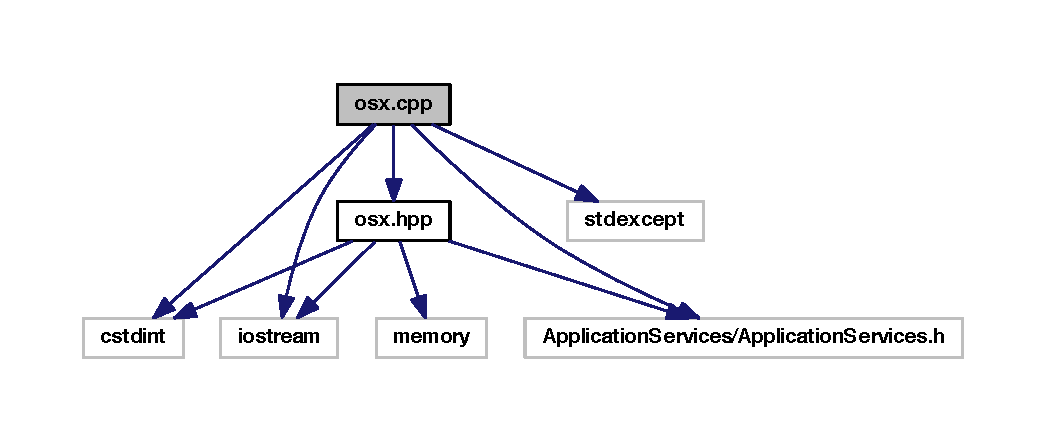
\includegraphics[width=350pt]{osx_8cpp__incl}
\end{center}
\end{figure}
\subsection*{Functions}
\begin{DoxyCompactItemize}
\item 
ostream \& \hyperlink{osx_8cpp_af829f2833c7596fe7b9cf41b58ae29b1}{operator$<$$<$} (ostream \&out, const mouse\-::\-Mouse\-State \&m)
\item 
ostream \& \hyperlink{osx_8cpp_ae35a0729fcf841f08cc4c1cd53038f97}{operator$<$$<$} (ostream \&out, const C\-G\-Color\-Space\-Ref \&color\-Space)
\begin{DoxyCompactList}\small\item\em Print {\ttfamily C\-G\-Color\-Space\-Ref} info. \end{DoxyCompactList}\item 
ostream \& \hyperlink{osx_8cpp_ac2540fce1dc9490db082314832db4a6a}{operator$<$$<$} (ostream \&out, const C\-G\-Image\-Ref \&im\-Ref)
\begin{DoxyCompactList}\small\item\em Print {\ttfamily C\-G\-Image\-Ref} info. \end{DoxyCompactList}\end{DoxyCompactItemize}


\subsection{Function Documentation}
\hypertarget{osx_8cpp_af829f2833c7596fe7b9cf41b58ae29b1}{\index{osx.\-cpp@{osx.\-cpp}!operator$<$$<$@{operator$<$$<$}}
\index{operator$<$$<$@{operator$<$$<$}!osx.cpp@{osx.\-cpp}}
\subsubsection[{operator$<$$<$}]{\setlength{\rightskip}{0pt plus 5cm}ostream\& operator$<$$<$ (
\begin{DoxyParamCaption}
\item[{ostream \&}]{out, }
\item[{const mouse\-::\-Mouse\-State \&}]{m}
\end{DoxyParamCaption}
)}}\label{osx_8cpp_af829f2833c7596fe7b9cf41b58ae29b1}
\hypertarget{osx_8cpp_ae35a0729fcf841f08cc4c1cd53038f97}{\index{osx.\-cpp@{osx.\-cpp}!operator$<$$<$@{operator$<$$<$}}
\index{operator$<$$<$@{operator$<$$<$}!osx.cpp@{osx.\-cpp}}
\subsubsection[{operator$<$$<$}]{\setlength{\rightskip}{0pt plus 5cm}ostream\& operator$<$$<$ (
\begin{DoxyParamCaption}
\item[{ostream \&}]{out, }
\item[{const C\-G\-Color\-Space\-Ref \&}]{color\-Space}
\end{DoxyParamCaption}
)}}\label{osx_8cpp_ae35a0729fcf841f08cc4c1cd53038f97}


Print {\ttfamily C\-G\-Color\-Space\-Ref} info. 

\hypertarget{osx_8cpp_ac2540fce1dc9490db082314832db4a6a}{\index{osx.\-cpp@{osx.\-cpp}!operator$<$$<$@{operator$<$$<$}}
\index{operator$<$$<$@{operator$<$$<$}!osx.cpp@{osx.\-cpp}}
\subsubsection[{operator$<$$<$}]{\setlength{\rightskip}{0pt plus 5cm}ostream\& operator$<$$<$ (
\begin{DoxyParamCaption}
\item[{ostream \&}]{out, }
\item[{const C\-G\-Image\-Ref \&}]{im\-Ref}
\end{DoxyParamCaption}
)}}\label{osx_8cpp_ac2540fce1dc9490db082314832db4a6a}


Print {\ttfamily C\-G\-Image\-Ref} info. 


\hypertarget{osx_8hpp}{\section{osx.\-hpp File Reference}
\label{osx_8hpp}\index{osx.\-hpp@{osx.\-hpp}}
}
{\ttfamily \#include $<$cstdint$>$}\\*
{\ttfamily \#include $<$iostream$>$}\\*
{\ttfamily \#include $<$memory$>$}\\*
{\ttfamily \#include $<$Application\-Services/\-Application\-Services.\-h$>$}\\*
{\ttfamily \#include \char`\"{}mouse.\-hpp\char`\"{}}\\*
{\ttfamily \#include \char`\"{}kmath.\-hpp\char`\"{}}\\*
Include dependency graph for osx.\-hpp\-:
\nopagebreak
\begin{figure}[H]
\begin{center}
\leavevmode
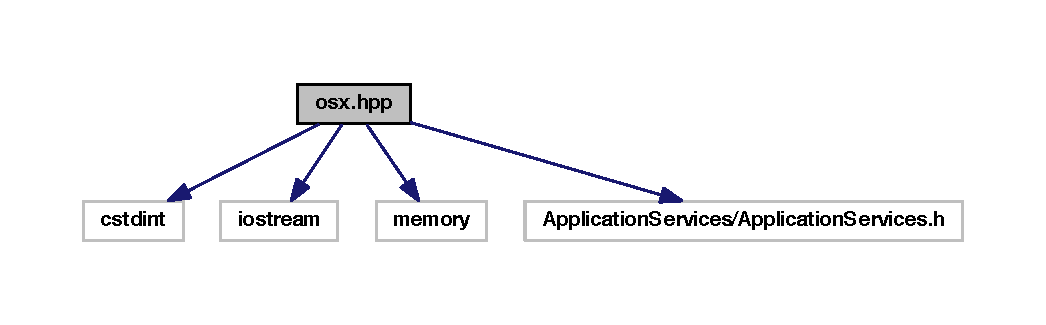
\includegraphics[width=350pt]{osx_8hpp__incl}
\end{center}
\end{figure}
This graph shows which files directly or indirectly include this file\-:\nopagebreak
\begin{figure}[H]
\begin{center}
\leavevmode
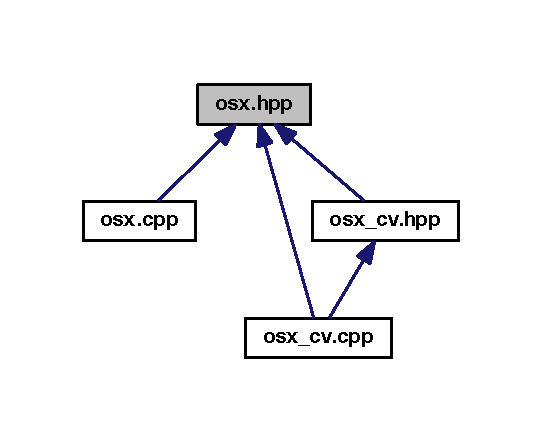
\includegraphics[width=260pt]{osx_8hpp__dep__incl}
\end{center}
\end{figure}
\subsection*{Classes}
\begin{DoxyCompactItemize}
\item 
struct \hyperlink{structosx_1_1disp_1_1_image}{osx\-::disp\-::\-Image}
\begin{DoxyCompactList}\small\item\em Memory-\/managed wrapper aronud {\ttfamily C\-G\-Image\-Ref} using a {\ttfamily shared\-\_\-ptr}. \end{DoxyCompactList}\end{DoxyCompactItemize}
\subsection*{Namespaces}
\begin{DoxyCompactItemize}
\item 
namespace \hyperlink{namespaceosx}{osx}
\begin{DoxyCompactList}\small\item\em O\-S\-X-\/specific utilities. \end{DoxyCompactList}\item 
namespace \hyperlink{namespaceosx_1_1mouse}{osx\-::mouse}
\begin{DoxyCompactList}\small\item\em Utilities for controlling the mouse. \end{DoxyCompactList}\item 
namespace \hyperlink{namespaceosx_1_1disp}{osx\-::disp}
\begin{DoxyCompactList}\small\item\em Functions for extracting the display image. \end{DoxyCompactList}\end{DoxyCompactItemize}
\subsection*{Defines}
\begin{DoxyCompactItemize}
\item 
\#define \hyperlink{osx_8hpp_ac041cfa66801dc389105798b67525f1e}{U\-N\-U\-S\-E\-D\-\_\-\-V\-A\-R}
\end{DoxyCompactItemize}
\subsection*{Enumerations}
\begin{DoxyCompactItemize}
\item 
enum \hyperlink{namespaceosx_1_1disp_a63adf9b0b0b0365ec428dd44fc30c659}{osx\-::disp\-::\-R\-G\-B\-Type} \{ \hyperlink{namespaceosx_1_1disp_a63adf9b0b0b0365ec428dd44fc30c659ab96ecb2ad3c69bf9019d7ed4253603b1}{osx\-::disp\-::\-C\-O\-L\-O\-R\-\_\-\-B\-G\-R}, 
\hyperlink{namespaceosx_1_1disp_a63adf9b0b0b0365ec428dd44fc30c659a307b3e319b6708774c7672d7efc04d0d}{osx\-::disp\-::\-C\-O\-L\-O\-R\-\_\-\-A\-R\-G\-B}, 
\hyperlink{namespaceosx_1_1disp_a63adf9b0b0b0365ec428dd44fc30c659aefca227dbfbf6803b1248aceeaa187b7}{osx\-::disp\-::\-C\-O\-L\-O\-R\-\_\-\-R\-G\-B\-A}
 \}
\end{DoxyCompactItemize}
\subsection*{Functions}
\begin{DoxyCompactItemize}
\item 
{\footnotesize template$<$typename T $>$ }\\C\-G\-Point \hyperlink{namespaceosx_abf7318d332d5e87088a270877f3da1ee}{osx\-::to\-C\-G\-Pt} (\hyperlink{structkmath_1_1_point}{kmath\-::\-Point}$<$ T $>$ pt)
\item 
\hyperlink{namespacekmath_ad80aa80b21a1aeadbd484a0fc56f4e95}{kmath\-::\-Point\-F} \hyperlink{namespaceosx_a37f829bcbe1e218b01dafeb711bd9d42}{osx\-::to\-Pt} (C\-G\-Point pt)
\item 
void \hyperlink{namespaceosx_1_1mouse_a96fc2b2983c0d9ee610ca9404ccc0506}{osx\-::mouse\-::move} (C\-G\-Point pos)
\begin{DoxyCompactList}\small\item\em Move cursor to {\ttfamily pos}. \end{DoxyCompactList}\item 
void \hyperlink{namespaceosx_1_1mouse_a8a25c1e4fda52095a4e113b2832777da}{osx\-::mouse\-::down} (\hyperlink{namespacemouse_af85c842f9410a5f81fe933360fb19bc4}{ms\-::\-Button} button, C\-G\-Point pos)
\begin{DoxyCompactList}\small\item\em Simulate a mouse down event at {\ttfamily pos}. \end{DoxyCompactList}\item 
void \hyperlink{namespaceosx_1_1mouse_a40b06e2da73d0ee062a669cdbcd6e4ef}{osx\-::mouse\-::up} (\hyperlink{namespacemouse_af85c842f9410a5f81fe933360fb19bc4}{ms\-::\-Button} button, C\-G\-Point pos)
\begin{DoxyCompactList}\small\item\em Simulate a mouse up event at {\ttfamily pos}. \end{DoxyCompactList}\item 
void \hyperlink{namespaceosx_1_1mouse_a127098ef29a5e3b824fdc2376e89f557}{osx\-::mouse\-::click} (\hyperlink{namespacemouse_af85c842f9410a5f81fe933360fb19bc4}{ms\-::\-Button} button, C\-G\-Point pos)
\begin{DoxyCompactList}\small\item\em Simulate a mouse click (button down, then up) event at {\ttfamily pos}. \end{DoxyCompactList}\item 
void \hyperlink{namespaceosx_1_1mouse_a49c625169ee20a981c56b3accf095605}{osx\-::mouse\-::drag} (\hyperlink{namespacemouse_af85c842f9410a5f81fe933360fb19bc4}{ms\-::\-Button} button, C\-G\-Point start\-Pos, C\-G\-Point end\-Pos)
\begin{DoxyCompactList}\small\item\em Simulate a mouse drag event at from {\ttfamily start\-Pos} to {\ttfamily end\-Pos}. \end{DoxyCompactList}\item 
Image \hyperlink{namespaceosx_1_1disp_a7d7872e070a2742dc7408ef1e56f7960}{osx\-::disp\-::get\-Screen} ()
\begin{DoxyCompactList}\small\item\em Return the current screen. \end{DoxyCompactList}\item 
ostream \& \hyperlink{osx_8hpp_ae35a0729fcf841f08cc4c1cd53038f97}{operator$<$$<$} (ostream \&out, const C\-G\-Color\-Space\-Ref \&color\-Space)
\begin{DoxyCompactList}\small\item\em Print {\ttfamily C\-G\-Color\-Space\-Ref} info. \end{DoxyCompactList}\item 
ostream \& \hyperlink{osx_8hpp_ac2540fce1dc9490db082314832db4a6a}{operator$<$$<$} (ostream \&out, const C\-G\-Image\-Ref \&im\-Ref)
\begin{DoxyCompactList}\small\item\em Print {\ttfamily C\-G\-Image\-Ref} info. \end{DoxyCompactList}\end{DoxyCompactItemize}


\subsection{Define Documentation}
\hypertarget{osx_8hpp_ac041cfa66801dc389105798b67525f1e}{\index{osx.\-hpp@{osx.\-hpp}!U\-N\-U\-S\-E\-D\-\_\-\-V\-A\-R@{U\-N\-U\-S\-E\-D\-\_\-\-V\-A\-R}}
\index{U\-N\-U\-S\-E\-D\-\_\-\-V\-A\-R@{U\-N\-U\-S\-E\-D\-\_\-\-V\-A\-R}!osx.hpp@{osx.\-hpp}}
\subsubsection[{U\-N\-U\-S\-E\-D\-\_\-\-V\-A\-R}]{\setlength{\rightskip}{0pt plus 5cm}\#define {\bf U\-N\-U\-S\-E\-D\-\_\-\-V\-A\-R}}}\label{osx_8hpp_ac041cfa66801dc389105798b67525f1e}


\subsection{Function Documentation}
\hypertarget{osx_8hpp_ae35a0729fcf841f08cc4c1cd53038f97}{\index{osx.\-hpp@{osx.\-hpp}!operator$<$$<$@{operator$<$$<$}}
\index{operator$<$$<$@{operator$<$$<$}!osx.hpp@{osx.\-hpp}}
\subsubsection[{operator$<$$<$}]{\setlength{\rightskip}{0pt plus 5cm}ostream\& operator$<$$<$ (
\begin{DoxyParamCaption}
\item[{ostream \&}]{out, }
\item[{const C\-G\-Color\-Space\-Ref \&}]{color\-Space}
\end{DoxyParamCaption}
)}}\label{osx_8hpp_ae35a0729fcf841f08cc4c1cd53038f97}


Print {\ttfamily C\-G\-Color\-Space\-Ref} info. 

\hypertarget{osx_8hpp_ac2540fce1dc9490db082314832db4a6a}{\index{osx.\-hpp@{osx.\-hpp}!operator$<$$<$@{operator$<$$<$}}
\index{operator$<$$<$@{operator$<$$<$}!osx.hpp@{osx.\-hpp}}
\subsubsection[{operator$<$$<$}]{\setlength{\rightskip}{0pt plus 5cm}ostream\& operator$<$$<$ (
\begin{DoxyParamCaption}
\item[{ostream \&}]{out, }
\item[{const C\-G\-Image\-Ref \&}]{im\-Ref}
\end{DoxyParamCaption}
)}}\label{osx_8hpp_ac2540fce1dc9490db082314832db4a6a}


Print {\ttfamily C\-G\-Image\-Ref} info. 


\hypertarget{seq_8hpp}{\section{seq.\-hpp File Reference}
\label{seq_8hpp}\index{seq.\-hpp@{seq.\-hpp}}
}
{\ttfamily \#include $<$cmath$>$}\\*
{\ttfamily \#include $<$cstddef$>$}\\*
{\ttfamily \#include $<$stdexcept$>$}\\*
{\ttfamily \#include $<$iostream$>$}\\*
{\ttfamily \#include $<$algorithm$>$}\\*
{\ttfamily \#include $<$iterator$>$}\\*
{\ttfamily \#include $<$utility$>$}\\*
{\ttfamily \#include \char`\"{}kmath.\-hpp\char`\"{}}\\*
Include dependency graph for seq.\-hpp\-:\nopagebreak
\begin{figure}[H]
\begin{center}
\leavevmode
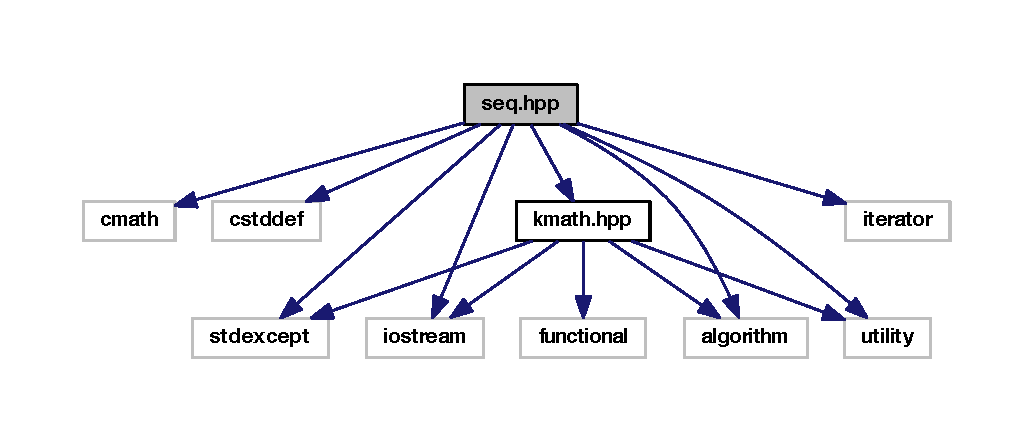
\includegraphics[width=350pt]{seq_8hpp__incl}
\end{center}
\end{figure}
This graph shows which files directly or indirectly include this file\-:\nopagebreak
\begin{figure}[H]
\begin{center}
\leavevmode
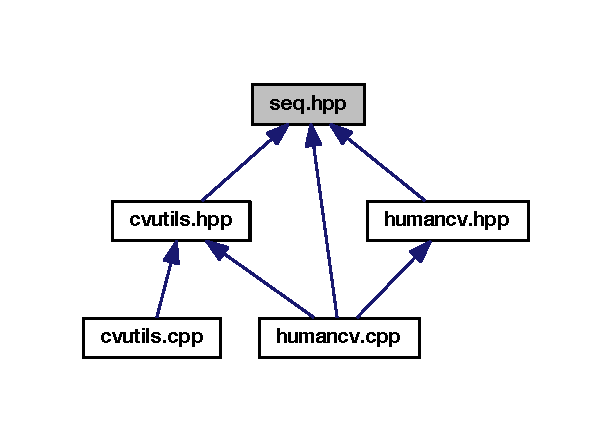
\includegraphics[width=243pt]{seq_8hpp__dep__incl}
\end{center}
\end{figure}
\subsection*{Classes}
\begin{DoxyCompactItemize}
\item 
struct \hyperlink{structseq_1_1_elem_view}{seq\-::\-Elem\-View$<$ Seq\-T $>$}
\begin{DoxyCompactList}\small\item\em Provides a reference and an index of an element in a sequence. \end{DoxyCompactList}\item 
struct \hyperlink{structseq_1_1_wrapped_seq}{seq\-::\-Wrapped\-Seq$<$ Seq\-T $>$}
\begin{DoxyCompactList}\small\item\em Sequence wrapper that supports wrap-\/around indexing -\/ all accessors will accept negative and out-\/of-\/bound indices and wrap around. \end{DoxyCompactList}\item 
class \hyperlink{classseq_1_1math_1_1_x_range_iterator}{seq\-::math\-::\-X\-Range\-Iterator$<$ Num\-T $>$}
\begin{DoxyCompactList}\small\item\em Lazy iterator used for X\-Range(), usually not necessary to use directly. \end{DoxyCompactList}\item 
struct \hyperlink{structseq_1_1math_1_1_x_range}{seq\-::math\-::\-X\-Range$<$ Num\-T $>$}
\begin{DoxyCompactList}\small\item\em Represent a lazily-\/evaluated range of numbers. \end{DoxyCompactList}\end{DoxyCompactItemize}
\subsection*{Namespaces}
\begin{DoxyCompactItemize}
\item 
namespace \hyperlink{namespaceseq}{seq}
\begin{DoxyCompactList}\small\item\em Generic sequence operations and structures. \end{DoxyCompactList}\item 
namespace \hyperlink{namespaceseq_1_1functional}{seq\-::functional}
\begin{DoxyCompactList}\small\item\em Functions commonly used in functional programming. \end{DoxyCompactList}\item 
namespace \hyperlink{namespaceseq_1_1math}{seq\-::math}
\begin{DoxyCompactList}\small\item\em Mathematical operations on sequences, and sequence structures. \end{DoxyCompactList}\end{DoxyCompactItemize}
\subsection*{Functions}
\begin{DoxyCompactItemize}
\item 
{\footnotesize template$<$class Seq\-T , typename Operand\-T $>$ }\\Seq\-T \& \hyperlink{seq_8hpp_a21a5aae4d520e12d3c987499aea2c0c4}{operator$\ast$=} (Seq\-T \&s, const Operand\-T \&e)
\begin{DoxyCompactList}\small\item\em Multiply each element in a sequence by {\ttfamily e}. \end{DoxyCompactList}\item 
{\footnotesize template$<$class Seq\-T , typename Operand\-T $>$ }\\Seq\-T \& \hyperlink{seq_8hpp_acf7f6f44050c057ff8e397070f2c497b}{operator/=} (Seq\-T \&s, const Operand\-T \&e)
\begin{DoxyCompactList}\small\item\em Divide each element in a sequence by {\ttfamily e}. \end{DoxyCompactList}\item 
size\-\_\-t \hyperlink{namespaceseq_a9f008982bf05fc256d4b035890744c77}{seq\-::\-\_\-real\-I} (int i, size\-\_\-t sz)
\begin{DoxyCompactList}\small\item\em Get the wrapped index to an array of size {\ttfamily sz}. \end{DoxyCompactList}\item 
size\-\_\-t \hyperlink{namespaceseq_ae4290a190db34f394330d88a5de8f2a7}{seq\-::\-\_\-real\-I\-Dist} (size\-\_\-t left\-I, size\-\_\-t right\-I, size\-\_\-t sz)
\begin{DoxyCompactList}\small\item\em Get the wrapped distance between left and right indices in an array of size {\ttfamily sz}. \end{DoxyCompactList}\item 
{\footnotesize template$<$class Seq\-T $>$ }\\Slice$<$ typename Seq\-T\-::iterator $>$ \hyperlink{namespaceseq_a01ecaea35db083541a258a05ac8c1d30}{seq\-::sl} (Seq\-T \&in, int i1, int i2)
\begin{DoxyCompactList}\small\item\em Get slice of sequence as a pair of iterators. \end{DoxyCompactList}\item 
{\footnotesize template$<$class In\-Seq\-T , class Out\-Seq\-T , typename \-\_\-\-Func\-T $>$ }\\Out\-Seq\-T \& \hyperlink{namespaceseq_1_1functional_ad36a538cd982a860de04e7f4af03bc4c}{seq\-::functional\-::map} (const \-\_\-\-Func\-T \&func, const In\-Seq\-T \&in, Out\-Seq\-T \&out)
\item 
{\footnotesize template$<$class In\-Seq\-T , class Out\-Seq\-T  = In\-Seq\-T, typename \-\_\-\-Func\-T $>$ }\\Out\-Seq\-T \hyperlink{namespaceseq_1_1functional_ab95c352080a36fe07cb04fe95b95caf8}{seq\-::functional\-::map} (const \-\_\-\-Func\-T \&func, const In\-Seq\-T \&in)
\item 
{\footnotesize template$<$class In\-Seq\-T , class Out\-Seq\-T , typename \-\_\-\-Func\-T $>$ }\\Out\-Seq\-T \& \hyperlink{namespaceseq_1_1functional_a5054f153ed880f89b744eec7aab118cf}{seq\-::functional\-::filter} (const \-\_\-\-Func\-T \&test, const In\-Seq\-T \&in, Out\-Seq\-T \&out)
\item 
{\footnotesize template$<$class In\-Seq\-T , class Out\-Seq\-T  = In\-Seq\-T, typename \-\_\-\-Func\-T $>$ }\\Out\-Seq\-T \hyperlink{namespaceseq_1_1functional_af3c889426da274197c74d0ec794072ff}{seq\-::functional\-::filter} (const \-\_\-\-Func\-T \&test, const In\-Seq\-T \&in)
\item 
{\footnotesize template$<$class Seq\-T , typename \-\_\-\-Func\-T $>$ }\\bool \hyperlink{namespaceseq_1_1functional_aadc273f6584110ccd147c612a2c315ab}{seq\-::functional\-::any} (const \-\_\-\-Func\-T \&test, const Seq\-T \&in)
\item 
{\footnotesize template$<$class Iter\-T , typename \-\_\-\-Func\-T $>$ }\\bool \hyperlink{namespaceseq_1_1functional_af131c7ae7d3ef6731a5e1fb71a8177aa}{seq\-::functional\-::any} (const \-\_\-\-Func\-T \&test, const Slice$<$ Iter\-T $>$ \&its)
\item 
{\footnotesize template$<$class Seq\-T , typename \-\_\-\-Func\-T $>$ }\\bool \hyperlink{namespaceseq_1_1functional_a2ffd96ef955260495f894c6eee90983c}{seq\-::functional\-::all} (const \-\_\-\-Func\-T \&test, const Seq\-T \&in)
\item 
{\footnotesize template$<$class Iter\-T , typename \-\_\-\-Func\-T $>$ }\\bool \hyperlink{namespaceseq_1_1functional_a6758cc8e1072ff3e3c0c32f121c879f4}{seq\-::functional\-::all} (const \-\_\-\-Func\-T \&test, const Slice$<$ Iter\-T $>$ \&its)
\item 
{\footnotesize template$<$typename Num\-T $>$ }\\X\-Range$<$ Num\-T $>$ \hyperlink{namespaceseq_1_1math_abfe793e999a374a4d5e6b1ef3f268b59}{seq\-::math\-::xrange} (Num\-T low, Num\-T high, Num\-T step=1, bool inclusive=false)
\begin{DoxyCompactList}\small\item\em Return {\ttfamily \hyperlink{structseq_1_1math_1_1_x_range}{X\-Range}} sequence, similar to Python's \char`\"{}xrange\char`\"{}. \end{DoxyCompactList}\item 
{\footnotesize template$<$typename Num\-T $>$ }\\X\-Range$<$ Num\-T $>$ \hyperlink{namespaceseq_1_1math_a4f2c47e50ba86a80778ccebd31d7fa16}{seq\-::math\-::xrange} (Num\-T high, bool inclusive=false)
\item 
{\footnotesize template$<$typename Num\-T , class Seq\-T $>$ }\\Seq\-T \& \hyperlink{namespaceseq_1_1math_a6bd86d848fb47f455aff84c38c175ea4}{seq\-::math\-::range} (Num\-T low, Num\-T high, Seq\-T \&out, Num\-T step=1)
\begin{DoxyCompactList}\small\item\em Construct a sequence of numbers from low to high with optional step. \end{DoxyCompactList}\item 
{\footnotesize template$<$typename Num\-T , class Seq\-T $>$ }\\Seq\-T \& \hyperlink{namespaceseq_1_1math_ae9b127e8277c6c390b99c4a1195dc087}{seq\-::math\-::range} (Num\-T high, Seq\-T \&out)
\begin{DoxyCompactList}\small\item\em Construct a sequence of numbers from 0 to high with step=1. \end{DoxyCompactList}\item 
{\footnotesize template$<$class Seq\-T $>$ }\\Seq\-T\-::value\-\_\-type \hyperlink{namespaceseq_1_1math_a27179daf6ca9a8d85434eda531fa134e}{seq\-::math\-::sum} (const Seq\-T \&in)
\begin{DoxyCompactList}\small\item\em Return the sum of sequence elements. \end{DoxyCompactList}\item 
{\footnotesize template$<$class Seq\-T $>$ }\\Seq\-T\-::value\-\_\-type \hyperlink{namespaceseq_1_1math_ab019165412bf99555adfeaaaa86f319f}{seq\-::math\-::mean} (const Seq\-T \&in)
\begin{DoxyCompactList}\small\item\em Return the arithmetic mean of sequence elements. \end{DoxyCompactList}\item 
{\footnotesize template$<$class Seq\-T $>$ }\\ostream \& \hyperlink{seq_8hpp_a25fc1874bf51d15a3fdfc0f63f75caa1}{operator$<$$<$} (ostream \&out, const \hyperlink{structseq_1_1_elem_view}{seq\-::\-Elem\-View}$<$ Seq\-T $>$ \&e)
\item 
{\footnotesize template$<$class Seq\-T $>$ }\\ostream \& \hyperlink{seq_8hpp_a987930fe6565e46853fbeb408ea3949b}{operator$<$$<$} (ostream \&out, const \hyperlink{structseq_1_1_wrapped_seq}{seq\-::\-Wrapped\-Seq}$<$ Seq\-T $>$ \&s)
\item 
{\footnotesize template$<$typename Elem\-Type , template$<$ typename U, class Alloc=allocator$<$ U $>$$>$ class Seq\-Type$>$ }\\ostream \& \hyperlink{seq_8hpp_a29425033946ee1e964e62754a6de891d}{operator$<$$<$} (ostream \&out, const Seq\-Type$<$ Elem\-Type $>$ \&seq)
\begin{DoxyCompactList}\small\item\em Print each element of a container, surrounded by {\ttfamily \mbox{[}\mbox{]}} and separated by commas. \end{DoxyCompactList}\end{DoxyCompactItemize}


\subsection{Function Documentation}
\hypertarget{seq_8hpp_a21a5aae4d520e12d3c987499aea2c0c4}{\index{seq.\-hpp@{seq.\-hpp}!operator$\ast$=@{operator$\ast$=}}
\index{operator$\ast$=@{operator$\ast$=}!seq.hpp@{seq.\-hpp}}
\subsubsection[{operator$\ast$=}]{\setlength{\rightskip}{0pt plus 5cm}template$<$class Seq\-T , typename Operand\-T $>$ Seq\-T\& operator$\ast$= (
\begin{DoxyParamCaption}
\item[{Seq\-T \&}]{s, }
\item[{const Operand\-T \&}]{e}
\end{DoxyParamCaption}
)}}\label{seq_8hpp_a21a5aae4d520e12d3c987499aea2c0c4}


Multiply each element in a sequence by {\ttfamily e}. 

\hypertarget{seq_8hpp_acf7f6f44050c057ff8e397070f2c497b}{\index{seq.\-hpp@{seq.\-hpp}!operator/=@{operator/=}}
\index{operator/=@{operator/=}!seq.hpp@{seq.\-hpp}}
\subsubsection[{operator/=}]{\setlength{\rightskip}{0pt plus 5cm}template$<$class Seq\-T , typename Operand\-T $>$ Seq\-T\& operator/= (
\begin{DoxyParamCaption}
\item[{Seq\-T \&}]{s, }
\item[{const Operand\-T \&}]{e}
\end{DoxyParamCaption}
)}}\label{seq_8hpp_acf7f6f44050c057ff8e397070f2c497b}


Divide each element in a sequence by {\ttfamily e}. 

\hypertarget{seq_8hpp_a25fc1874bf51d15a3fdfc0f63f75caa1}{\index{seq.\-hpp@{seq.\-hpp}!operator$<$$<$@{operator$<$$<$}}
\index{operator$<$$<$@{operator$<$$<$}!seq.hpp@{seq.\-hpp}}
\subsubsection[{operator$<$$<$}]{\setlength{\rightskip}{0pt plus 5cm}template$<$class Seq\-T $>$ ostream\& operator$<$$<$ (
\begin{DoxyParamCaption}
\item[{ostream \&}]{out, }
\item[{const {\bf seq\-::\-Elem\-View}$<$ Seq\-T $>$ \&}]{e}
\end{DoxyParamCaption}
)}}\label{seq_8hpp_a25fc1874bf51d15a3fdfc0f63f75caa1}
\hypertarget{seq_8hpp_a987930fe6565e46853fbeb408ea3949b}{\index{seq.\-hpp@{seq.\-hpp}!operator$<$$<$@{operator$<$$<$}}
\index{operator$<$$<$@{operator$<$$<$}!seq.hpp@{seq.\-hpp}}
\subsubsection[{operator$<$$<$}]{\setlength{\rightskip}{0pt plus 5cm}template$<$class Seq\-T $>$ ostream\& operator$<$$<$ (
\begin{DoxyParamCaption}
\item[{ostream \&}]{out, }
\item[{const {\bf seq\-::\-Wrapped\-Seq}$<$ Seq\-T $>$ \&}]{s}
\end{DoxyParamCaption}
)}}\label{seq_8hpp_a987930fe6565e46853fbeb408ea3949b}
\hypertarget{seq_8hpp_a29425033946ee1e964e62754a6de891d}{\index{seq.\-hpp@{seq.\-hpp}!operator$<$$<$@{operator$<$$<$}}
\index{operator$<$$<$@{operator$<$$<$}!seq.hpp@{seq.\-hpp}}
\subsubsection[{operator$<$$<$}]{\setlength{\rightskip}{0pt plus 5cm}template$<$typename Elem\-Type , template$<$ typename U, class Alloc=allocator$<$ U $>$$>$ class Seq\-Type$>$ ostream\& operator$<$$<$ (
\begin{DoxyParamCaption}
\item[{ostream \&}]{out, }
\item[{const Seq\-Type$<$ Elem\-Type $>$ \&}]{seq}
\end{DoxyParamCaption}
)}}\label{seq_8hpp_a29425033946ee1e964e62754a6de891d}


Print each element of a container, surrounded by {\ttfamily \mbox{[}\mbox{]}} and separated by commas. 


\hypertarget{str_8cpp}{\section{str.\-cpp File Reference}
\label{str_8cpp}\index{str.\-cpp@{str.\-cpp}}
}
{\ttfamily \#include $<$string$>$}\\*
{\ttfamily \#include $<$stdexcept$>$}\\*
{\ttfamily \#include \char`\"{}str.\-hpp\char`\"{}}\\*
{\ttfamily \#include \char`\"{}io.\-hpp\char`\"{}}\\*
Include dependency graph for str.\-cpp\-:\nopagebreak
\begin{figure}[H]
\begin{center}
\leavevmode
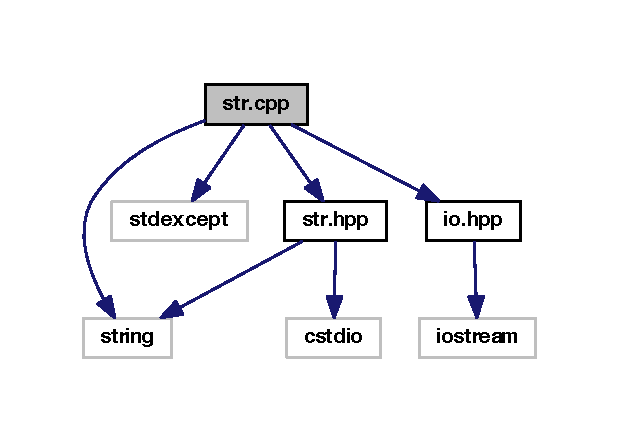
\includegraphics[width=297pt]{str_8cpp__incl}
\end{center}
\end{figure}

\hypertarget{str_8hpp}{\section{str.\-hpp File Reference}
\label{str_8hpp}\index{str.\-hpp@{str.\-hpp}}
}
{\ttfamily \#include $<$cstdio$>$}\\*
{\ttfamily \#include $<$string$>$}\\*
\subsection*{Namespaces}
\begin{DoxyCompactItemize}
\item 
namespace \hyperlink{namespacestr}{str}
\begin{DoxyCompactList}\small\item\em String utilities. \end{DoxyCompactList}\end{DoxyCompactItemize}
\subsection*{Defines}
\begin{DoxyCompactItemize}
\item 
\#define \hyperlink{str_8hpp_ad02d698209df17aef336d5633065c5ab}{str\-Fmt}(fmt,...)~(snprintf(\hyperlink{namespacestr_a51a7257ade189ec55f5d1c9da0f0e8b4}{str\-::\-\_\-buf}, 100, fmt, \-\_\-\-\_\-\-V\-A\-\_\-\-A\-R\-G\-S\-\_\-\-\_\-), \hyperlink{namespacestr_a51a7257ade189ec55f5d1c9da0f0e8b4}{str\-::\-\_\-buf})
\end{DoxyCompactItemize}
\subsection*{Functions}
\begin{DoxyCompactItemize}
\item 
string \hyperlink{namespacestr_a7b677ee9cce42c91dcd37d68b7fa04ac}{str\-::word\-Wrap} (string in, unsigned cols=80)  throw (length\-\_\-error)
\end{DoxyCompactItemize}
\subsection*{Variables}
\begin{DoxyCompactItemize}
\item 
char \hyperlink{namespacestr_a51a7257ade189ec55f5d1c9da0f0e8b4}{str\-::\-\_\-buf} \mbox{[}100\mbox{]}
\end{DoxyCompactItemize}


\subsection{Define Documentation}
\hypertarget{str_8hpp_ad02d698209df17aef336d5633065c5ab}{\index{str.\-hpp@{str.\-hpp}!str\-Fmt@{str\-Fmt}}
\index{str\-Fmt@{str\-Fmt}!str.hpp@{str.\-hpp}}
\subsubsection[{str\-Fmt}]{\setlength{\rightskip}{0pt plus 5cm}\#define {\bf str\-Fmt}(
\begin{DoxyParamCaption}
\item[{}]{fmt, }
\item[{}]{...}
\end{DoxyParamCaption}
)~(snprintf({\bf str\-::\-\_\-buf}, 100, fmt, \-\_\-\-\_\-\-V\-A\-\_\-\-A\-R\-G\-S\-\_\-\-\_\-), {\bf str\-::\-\_\-buf})}}\label{str_8hpp_ad02d698209df17aef336d5633065c5ab}
Functional version of {\ttfamily snprintf}.

Yes, macros are evil, but this is so convenient. 
\hypertarget{thr_8hpp}{\section{thr.\-hpp File Reference}
\label{thr_8hpp}\index{thr.\-hpp@{thr.\-hpp}}
}
{\ttfamily \#include $<$deque$>$}\\*
{\ttfamily \#include $<$mutex$>$}\\*
Include dependency graph for thr.\-hpp\-:
\nopagebreak
\begin{figure}[H]
\begin{center}
\leavevmode
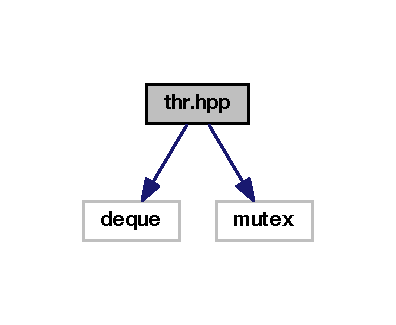
\includegraphics[width=190pt]{thr_8hpp__incl}
\end{center}
\end{figure}
\subsection*{Classes}
\begin{DoxyCompactItemize}
\item 
struct \hyperlink{structthr_1_1_queue}{thr\-::\-Queue$<$ T $>$}
\begin{DoxyCompactList}\small\item\em Producer-\/consumer queue. \end{DoxyCompactList}\end{DoxyCompactItemize}
\subsection*{Namespaces}
\begin{DoxyCompactItemize}
\item 
namespace \hyperlink{namespacethr}{thr}
\begin{DoxyCompactList}\small\item\em Multi-\/threading utilities. \end{DoxyCompactList}\end{DoxyCompactItemize}

\printindex
\end{document}
